\documentclass[NETN,manuscript]{stjour-new}
\setcounter{secnumdepth}{1}

%\usepackage{hyperref}
%  Environments

% Theorems, etc

\usepackage{microtype}
\usepackage{graphicx}
\usepackage{hyperref}
\usepackage{subfigure}
\usepackage{booktabs} % for professional tables
\usepackage{tikz-cd}
\usepackage{amsmath}
\usepackage{amsfonts}
\usepackage{algorithm}% http://ctan.org/pkg/algorithms
\usepackage{algpseudocode}
\usepackage{wrapfig,lipsum,booktabs}
\usepackage[ruled,vlined]{algorithm2e}
\usepackage{amsthm}
\newcommand{\comment}[1]{}
\newcommand{\preprocess}{\textsc{preprocess}}
\newcommand{\Cov}{\mathrm{Cov}}
\newtheorem{proposition}{Proposition}
\newtheorem{definition}{Definition}
\newcommand{\dataset}{\mathcal{Dataset}}
\newcommand{\E}{\mathbb{E}}

\newcommand{\mmp}[1]{\textcolor{red}{\em MMP: #1}}
\newcommand{\skcomment}[1]{({\color{blue}{SK's comment:}}\textbf{\color{blue}{#1}})}
%\setcounter{secnumdepth}{1}
% hyperref makes hyperlinks in the resulting PDF.
% If your build breaks (sometimes temporarily if a hyperlink spans a page)
% please comment out the following usepackage line and replace
% \usepackage{icml2019} with \usepackage[nohyperref]{icml2019} above.
\usepackage{hyperref}

\tikzset{%
  symbol/.style={
    draw=none,
    every to/.append style={
      edge node={node [sloped, allow upside down, auto=false]{$#1$}}
    },
  },
}

% Attempt to make hyperref and algorithmic work together better:
\newcommand{\theHalgorithm}{\arabic{algorithm}}




\newlength\Colsep
\setlength\Colsep{10pt}
%\usetikzlibrary{arrows.meta,
%                positioning
%                }
%\externaldocument[supp-]{Supplement.tex}

\newcommand{\smcomment}[1]{({\color{red}{Stefan's comment:}}\textbf{\color{red}{#1}})}
%\newcommand{\skcomment}[1]{({\color{blue}{SK's comment:}}\textbf{\color{blue}{#1}})}
\renewcommand\theadalign{bc}
\renewcommand\theadfont{\bfseries}
\renewcommand\theadgape{\Gape[4pt]}
\renewcommand\cellgape{\Gape[4pt]}

\makeatletter
\newcommand*{\addFileDependency}[1]{% argument=file name and extension
  \typeout{(#1)}% latexmk will find this if $recorder=0 (however, in that case, it will ignore #1 if it is a .aux or .pdf file etc and it exists! if it doesn't exist, it will appear in the list of dependents regardless)
  \@addtofilelist{#1}% if you want it to appear in \listfiles, not really necessary and latexmk doesn't use this
  \IfFileExists{#1}{}{\typeout{No file #1.}}% latexmk will find this message if #1 doesn't exist (yet)
}
\makeatother

\newcommand*{\myexternaldocument}[1]{%
    \externaldocument{#1}%
    \addFileDependency{#1.tex}%
    \addFileDependency{#1.aux}%
}
%\newcommand{\comment}[1]{}
%\myexternaldocument{Supplement}
\listfiles

\articletype{Research}

%\def\taupav{\tau_{\mathrm{Pav}}}

\begin{document}


\title{Modelling the cell-type specific mesoscale murine connectome with anterograde tracing experiments}

\author[Koelle et al]% shortened version for running head, optional
{Samson Koelle \affil{1,2}, Dana Mastrovito \affil{1}, Jennifer D Whitesell \affil{1}, Karla E Hirokawa \affil{1},  Hongkui Zeng\affil{1}, Marina Meila\affil{2}, Julie A Harris\affil{1}, Stefan Mihalas\affil{1}}

\affiliation{1}{Allen Institute for Brain Science, Seattle, WA, USA}

\affiliation{2}{Department of Statistics, University of Washington, Seattle, WA, USA}

\correspondingauthor{Stefan Mihalas}{stefanm@alleninstitute.org}

\keywords{[Connectivity, Cell-type, Mouse]}

\begin{abstract}
The Allen Mouse Brain Connectivity Atlas consists of anterograde tracing experiments targeting diverse structures and classes of projecting neurons.
Beyond regional anterograde tracing done in C57BL/6 wild type mice, a large fraction of experiments are performed using transgenic Cre-lines.
This allows access to cell-class specific whole brain connectivity information, with class defined by the transgenic lines.
However, even though the number of experiments is large, it does not come close to covering all existing cell classes in every area where they exist.
Here, we study how much we can fill in these gaps and estimate the cell-class specific connectivity function given the simplifying assumptions that nearby voxels have smoothly varying projections, but that these projection tensors can change sharply depending on the region and class of the projecting cells.

This paper describes the conversion of Cre-line tracer experiments into class-specific connectivity matrices representing the connection strengths between source and target structures.
We introduce and validate a novel statistical model for creation of connectivity matrices.
We extend the Nadaraya-Watson kernel learning method which we previously used to fill in spatial gaps to also fill in a gaps in cell-class connectivity information.
To do this, we construct a "cell-class space" based on class-specific averaged regionalized projections and combine smoothing in 3D space as well as in this abstract space to share information between similar neuron classes.
Using this method we construct a set of connectivity matrices using multiple levels of resolution at which discontinuities in connectivity are assumed. We show that the connectivities obtained from this model display expected cell-type and structure specific connectivities. 
We also show that the wild type connectivity matrix can be factored using a sparse set of factors, and analyze the informativeness of this latent variable model.

\end{abstract}

\begin{authorsummary}
Large-scale studies have described the connections between areas in multiple mammalian models in ever expanding detail.
Standard connectivity studies focus on the connection strength between areas.
However, when describing functions at a local circuit level, there is an increasing focus on cell types.
We have recently described the importance of connection types in the cortico-thalamic system, which allows an unsupervised discovery of its hierarchical organization.
In this study we focus on adding a dimension of connection type for a brain-wide mesoscopic connectivity model.
Even with our relatively massive dataset, the data in the cell type direction for connectivity is quite sparse, and we had to develop methods to more reliably extrapolate in such directions, and to estimate when such extrapolations are impossible.
This allows us to fill in such a connection type specific inter-areal connectivity matrix to the extent our data allows. 
While analyzing this complex connectivity, we observed that it can be described via a small set of factors. 
While not complete, this connectivity matrix represents a a categorical and quantitative improvement in mouse mesoscale connectivity models. 

\end{authorsummary}

\newpage

\section{Introduction}
 
The mammalian nervous system enables an extraordinary range of natural behaviors, and has inspired much of modern artificial intelligence.
Neural connections including those from one region to another form the architecture underlying this capability.
These connectivities vary by neuron type, as well as source (cell body) location and target (axonal projection) structures.
Thus, characterization of the relationship between neuron type and source and target structure is important for understanding the overall nervous system.

Viral tracing experiments - in which a viral vector expressing GFP is transduced into neural cells through stereotaxic injection - are a useful tool for mapping these connections on the mesoscale \citep{Chamberlin1998-hi,Harris2012-fw, Daigle2018-gd}.
The long range connections between different areas are generally formed by axons which travel from one region to another, and the GFP protein moves into the axon of the projecting neurons.
Two-photon tomography imaging can be used to determine the location and strength of the fluorescent signals in two-dimensional slices.
These locations can then be mapped back into three-dimensional space, and the signal may then be integrated over area into cubic voxels to give a finely-quantized three-dimensional fluorescence.

Several statistical models for the conversion of such experiment-specific signals into generalized estimates of connectivity strength have been proposed \citep{Oh2014-kh, Harris2016-fn, Gamanut2018-sd, Knox2019-ot}.
Of these, \citet{Oh2014-kh} and \citet{Knox2019-ot} provide a model for \textbf{regionalized connectivities}, which are voxel connectivities integrated by region.
The value of these models is that they provide some improvement over simply averaging the projection signals of injections in a given region.
However, these previous works only model connectivities observed in wild-type mice which are suboptimally suited to assessment of cell-type specific connectivity compared with fluorescence from Cre-recombinase induced eGFP expression in cell-types specified by the combination of transgenic mouse strain and transgene promoter \citep{Harris2019-mr}.
We generally refer to sets of so-targeted eGFP-expressing cells in tracing experiments as a \textbf{cell class} since they may contain multiple types.
For example, use of both wild-type and transgenic mice would give rise to cell-class specific experiments, albeit with different yet perhaps overlapping classes of cells.

Thus, this paper introduces a class-specific statistical model for anterograde tracing experiments that synthesizes the diverse set of \textbf{Cre-lines} described in \citet{Harris2019-mr}, and expands this model to the entire mouse brain.
Our model is a to-our-knowledge novel statistical estimator that takes into account both the spatial position of the labelled source, as well as the categorical cell class.
Like the previously state-of-the-art model in \citet{Knox2019-ot}, this model predicts regionalized connectivity as an average over positions within the structure, with nearby experiments given more weight.
However, our model weighs class-specific behavior in a particular structure against spatial position, so a nearby experiment specific to a similar cell-class is relatively up-weighted, while a nearby experiment specific to a dissimilar class is down-weighted.
This model outperforms the model of  \citet{Knox2019-ot} based on its ability to predict held-out experiments in leave-one-out cross-validation.
We use the trained model to estimate overall connectivity matrices for each assayed cell class.

The resulting cell-class specific connectivity is a directed weighted multigraph which can be represented as a tensor with missing values.
We do not give an exhaustive analysis of this data, but do establish a lower-limit of detection, verify several cell-type specific connectivity patterns found elsewhere in the literature, and show that these cell-type specific signals are behaving in expected ways.
We also decompose the wild-type connectivity matrix into factors representing latent connectivity patterns, which we call archetypes.
These components allow approximation of the regionalized connectivity using linear combinations of a small set of components.

Section \ref{sec:methods} gives information on the data and statistical methodology, and Section \ref{sec:results} presents our results.
These include connectivities, assessments of model fit, and subsequent biological and statistical analyses.
Additional information on our dataset, methods, and results are given in Supplemental Sections \ref{supp_sec:info}, \ref{supp_sec:methods}, and \ref{supp_sec:exp}, respectively.
\newpage
\section{Methods}
\label{sec:methods}

We estimate and analyze cell class-specific connectivity functions using models trained on murine brain viral tracing experiments.
This section describes the data used to generate the model, the model itself, the evaluation of the model against its alternatives, and the use of the model in creation of the connectivity estimate matrices.
It also includes background on the non-negative matrix factorization method used for decomposing the wild type connectivity matrix into latent factors.
Additional information about our data and methods are given in Supplemental Sections \ref{supp_sec:data} and \ref{supp_sec:methods}, respectively.

\newpage
\begin{figure}[H]
\subfloat[]{
\label{fig:mouse}
    
\includegraphics[width=0.3\textwidth]{figs/figure1a.png}}
\subfloat[]{
\label{fig:injproj}
    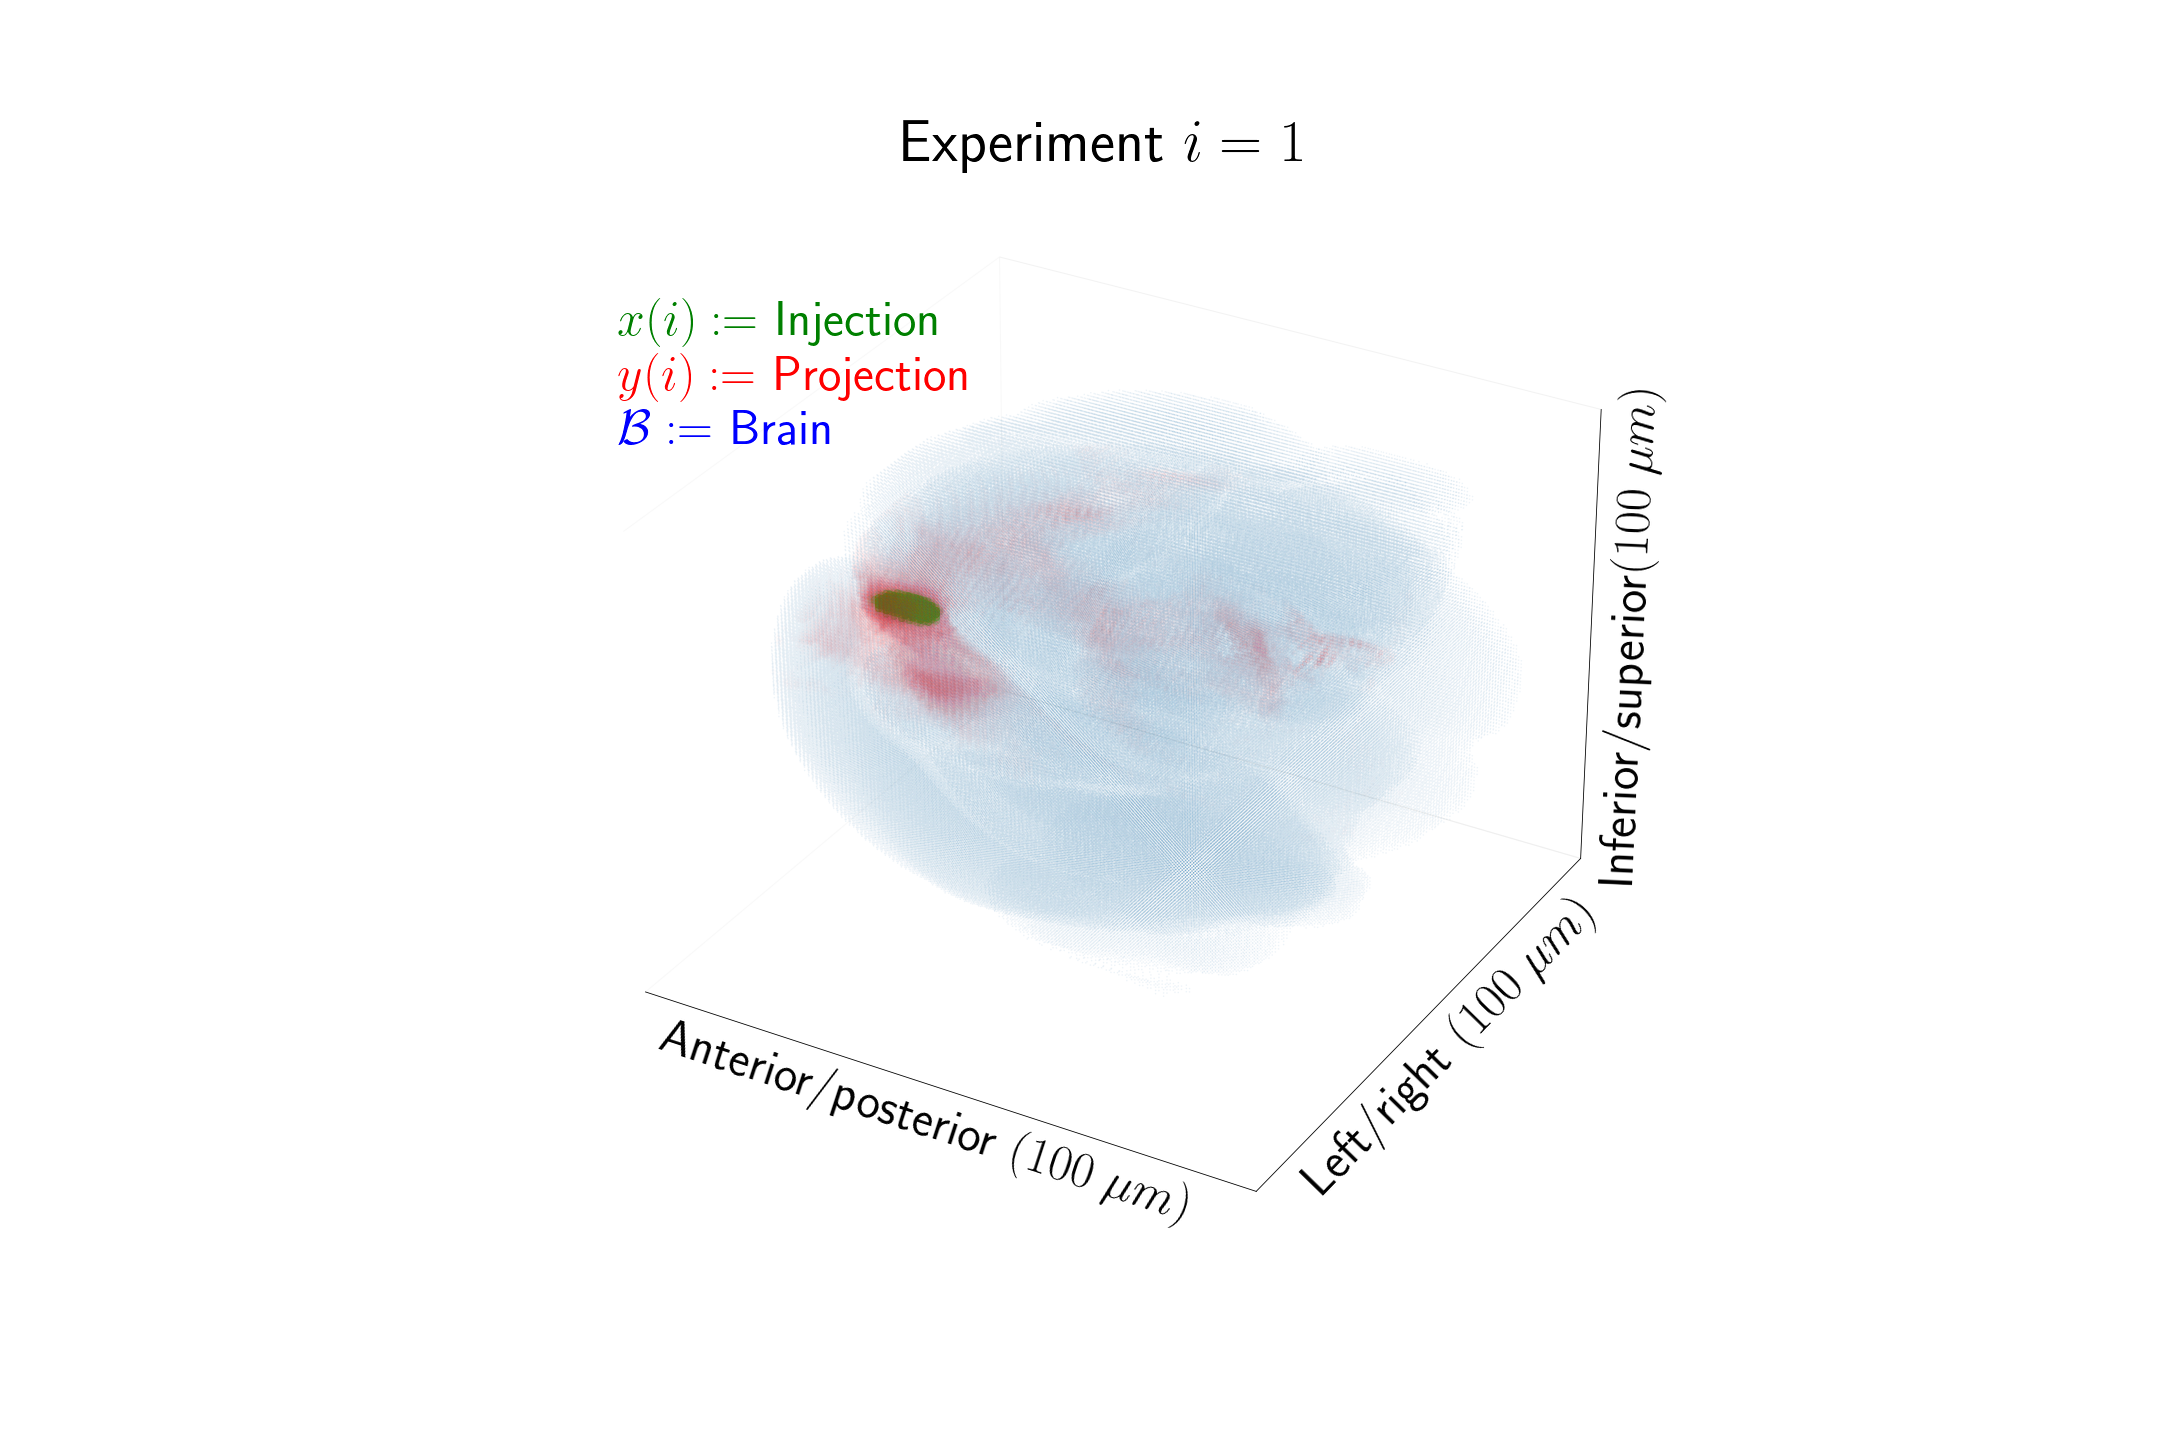
\includegraphics[width=0.4\textwidth]{figs/inj_proj_figure_v2.png}}
\subfloat[]{
\label{fig:segment}
    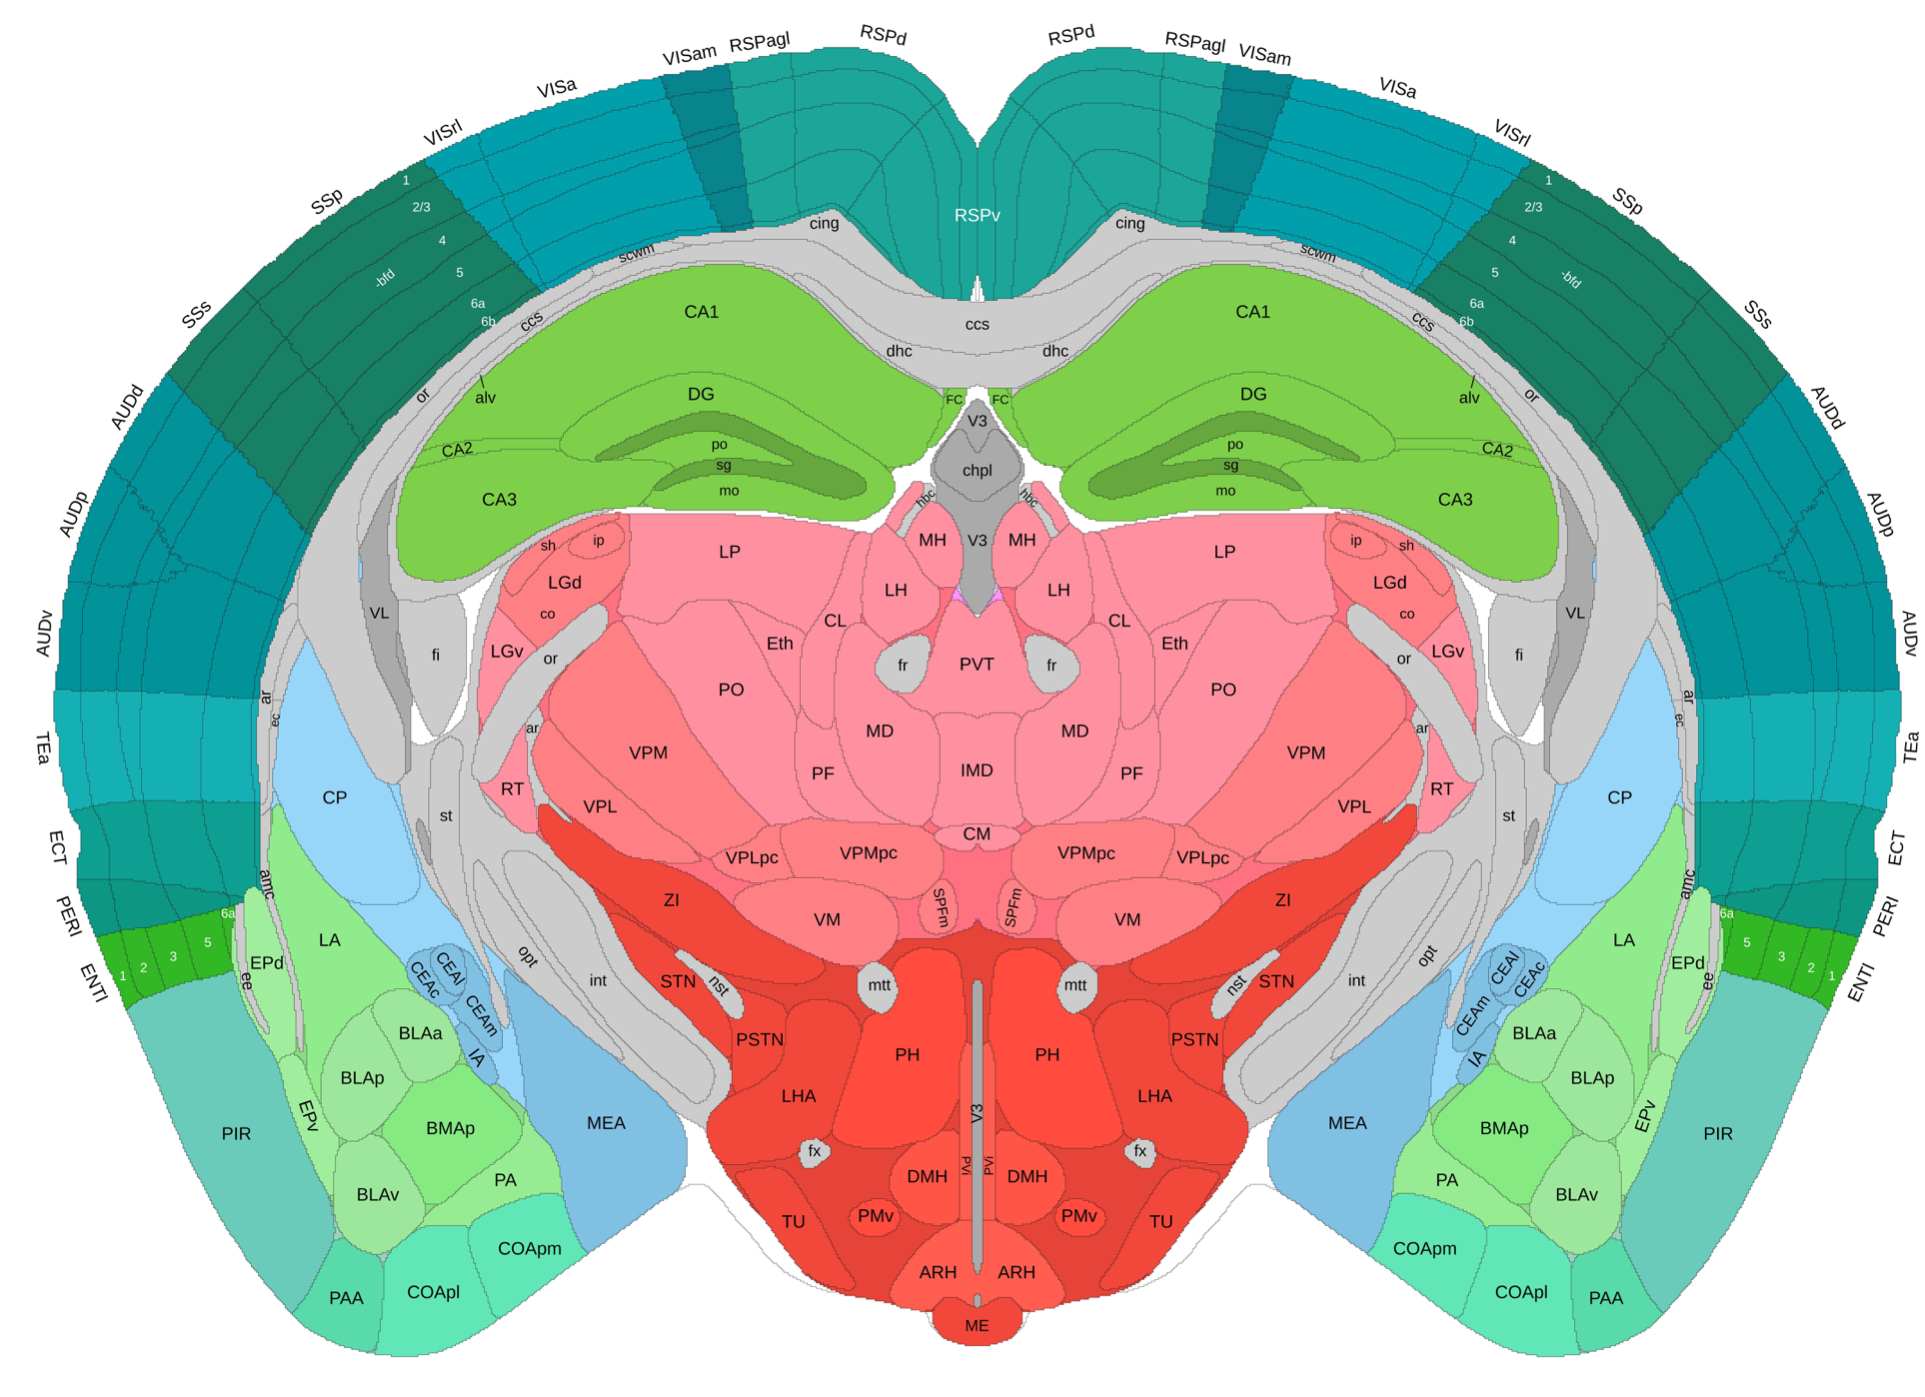
\includegraphics[width=0.3\textwidth]{figs/fig1c.png}}
    \newline
 \subfloat[]{
 \label{fig:ontology}
    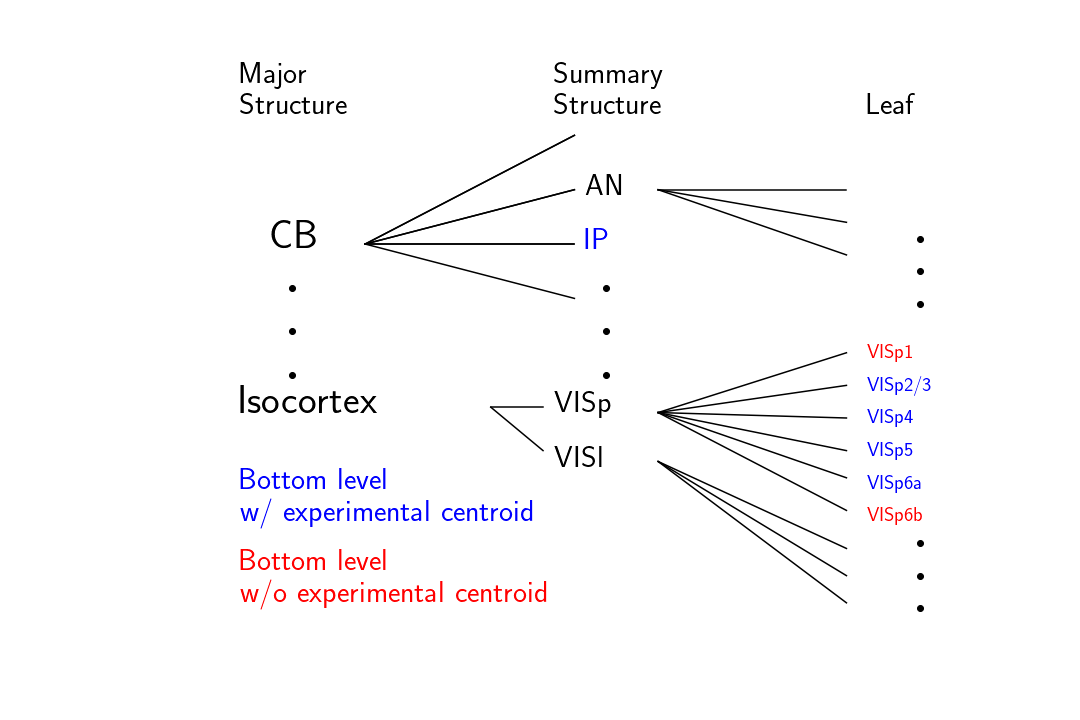
\includegraphics[width=0.35\textwidth]{figs/ontologyfigure.png}}
\subfloat[]{
 \label{fig:top}
    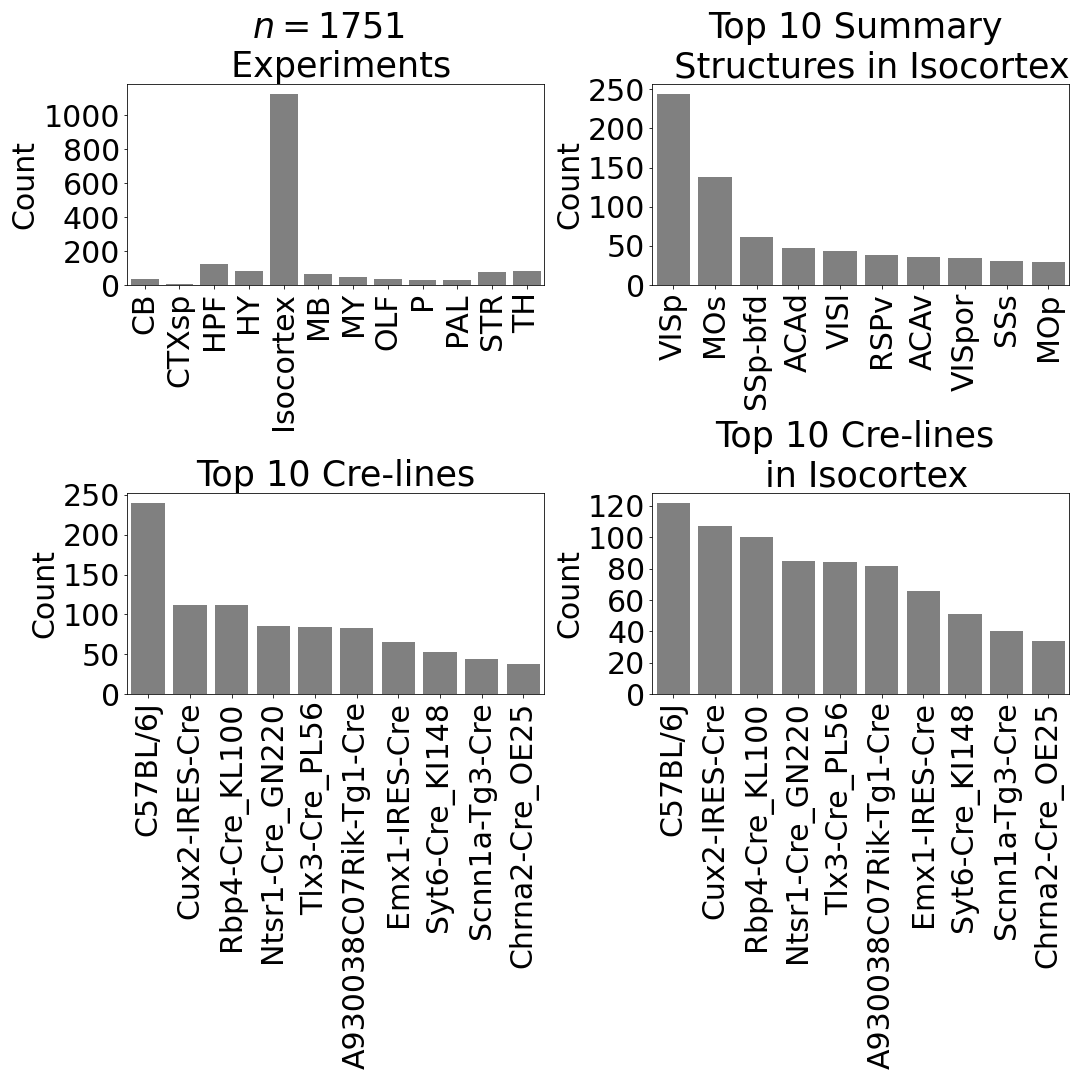
\includegraphics[width=0.35\textwidth]{figs/datasummary.png}}
\subfloat[]{
 \label{fig:combos}
    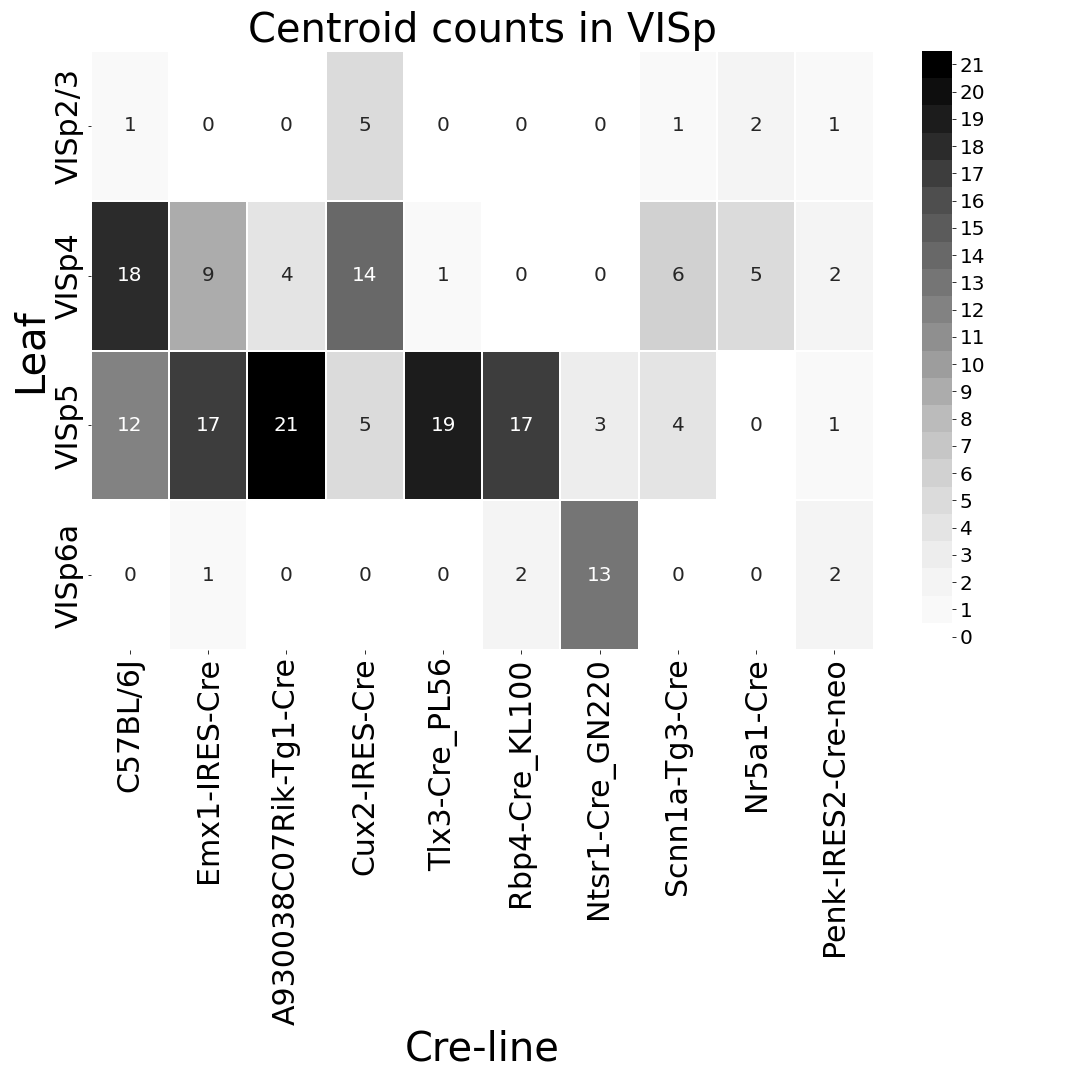
\includegraphics[width=0.35\textwidth]{figs/visp_counts.png}}   
    \caption{Experimental setting.  \ref{fig:mouse}  For each experiment, a Cre-dependent GFP-expressing transgene casette is transduced by stereotaxic injection into a Cre-driver mouse, followed by serial two-photon tomography imaging.
    \ref{fig:injproj} An example of the segmentation of projection (targets) and injection (source) for a single experiment. Within each brain (blue), injection (green) and projection (red) areas are determined via histological analysis and alignment to the Allen Common Coordinate Framework (CCF).
    \ref{fig:segment} Brain region parcellations within a coronal plane of CCFv3. \ref{fig:ontology} Explanation of nested structural ontology highlighting various levels of CCFv3 structure ontology.
    Lowest-level (leaf) structures are colored in blue, and structures without an injection centroid are colored in red.
    \ref{fig:top}  Abundances of tracer experiments by Cre-line and region of injection. \ref{fig:combos}  Co-occurrence of layer-specific centroids and Cre-lines within VISp.}
    \label{fig:data}
\end{figure}

\newpage

\subsection{Data}

Our dataset $\mathcal D$ consists of $n=1751$ publicly available murine brain viral tracing experiments from the Allen Mouse Brain Connectivity Atlas.
Figure \ref{fig:mouse} summarizes the experimental process used to generate this data.
In each experiment, a mouse is injected with an adeno-associated virus (AAV) encoding green fluorescent protein (GFP) into a single location in the brain.
Location of fluorescence is mediated by the location of the injection, the characteristics of the transgene, and the genotype of the mouse.
In particular, Cre-driver mice are engineered to express Cre under the control of a specific and single gene promoter.
This localizes expression of Cre to regions with certain transcriptomic cell-types signatures.
In such Cre-driver mice, we used a double-inverted floxed AAV to produce fluorescence that depends on Cre expression in infected cells.
To account for the complex cell-type targeting induced by a particular combination of Cre-driver genotype and GFP promoter, we refer to the combinations of cell-types targeted by a particular combination of AAV and Cre-driver mice as cell-classes.
For example, we include experiments from Cre-driver lines that selectively label cell classes located in distinct cortical layers or other nuclei across the whole brain.
By our definition, wild type mice transduced with constitutitively active GFP promoters induce fluorescence of a particularly broad cell class.

For each experiment, the fluorescent signal imaged after injection is aligned into the Allen Common Coordinate Framework (CCF) v3, a three-dimensional average template brain that is fully annotated with regional parcellations \cite{Wang2020-po}.
The whole brain imaging and registration procedures described in detail in \citet{Oh2014-kh, Kuan2015-zz} produce quantitative metrics of fluorescence discretized at the $100 \; \mu$m \textbf{voxel} level. 
Given an experiment, this image was histologically segmented by an analyst into \textit{injection} and \textit{projection} areas corresponding to areas containing somas, dendrites and axons or exclusively axons of the transfected neurons.
An example of a single experiment rendered in 3D is given in Figure \ref{fig:injproj}.
Given an experiment $i$, we represent injections and projections as functions $x(i),y(i) : \mathcal B \to \mathbb R_{\geq 0}$, where $\mathcal B \subset [1:132] \times [1:80] \times [1:104]$ corresponds to the subset of the $(1.32 \times 0.8 \times 1.04)$ cm rectangular space occupied by the standard voxelized mouse brain.
We also calculate injection centroids $c(i) \in \mathbb R^3$ and regionalized projections $y_{\mathcal T} (i) \in \mathbb R^{T} $ given by the sum of $y(i)$ in each region.
A description of these steps is in Supplemental Section \ref{supp_sec:dp}.

Our goal is the estimation of \textbf{regionalized connectivity} from one region to another.
A visual depiction of this region parcellation for a two-dimensional slice of the brain is given in Figure \ref{fig:segment}.
All structures annotated in the CCF belong to a hierarchically ordered ontology, with different areas of the brain are parcellated to differing finer depths within a hierarchical tree.
We denote the main levels of interest as major structures, summary structures, and layers.
Not every summary structure has a layer decomposition within this ontology, so we typically consider the finest possible regionalization - for example, layer within the cortex, and summary structure within the thalymus, and denote these structures as leafs.
As indicated in Figure \ref{fig:ontology}, the dataset used to generate the connectivity model reported in this paper contains certain combinations of region and cell class frequently, and others not at all.
A summary of the most frequently assayed cell classes and structures is given in Figures \ref{fig:top} and \ref{fig:combos}.
Since users of the connectivity matrices may be interested in particular combinations, or interested in the amount of data used to generate a particular connectivity estimate, we present this information about all experiments in Supplemental Section \ref*{supp_sec:data}.

\newpage

\subsection{Modeling Regionalized Connectivity}
\label{sec:modelling}

We define voxelized cell-class specific connectivity $f:  \mathcal V \times \mathcal B \times \mathbb \mathcal \to \mathbb R_{\geq 0}$ as giving the voxelized connectivity strength of a particular cell class from a source voxel to a target voxel.
In contrast to \citet{Knox2019-ot}, which only uses wild type C57BL/6J mice, our dataset has experiments targeting $|\mathcal V| = 114$ different combinations of Cre-driver mice and Cre-regulated AAV transgenes jointly denoted as $\mathcal V := \{v\}$.
As in \citet{Knox2019-ot}, we ultimately estimate an integrated regionalized connectivity defined with respect to a set of $S = 564$ source leafs $\mathcal S := \{ s\} $ and $T = 1123$ target leafs $\mathcal T := \{ t \}$, of which $1123 - 564  = 559$ are contralateral.
That is, we define
\begin{align*}
&\text{\textit {regionalized connectivity strength} } \mathcal C : \mathcal V \times \mathcal S \times \mathcal T \to \mathbb R_{\geq 0}  \text{ with } \mathcal C(v,s,t) = \sum_{l_{j} \in s} \sum_{l_{j'} \in  t} f(v,l_{j},l_{j'}), \\
&\text{\textit {normalized regionalized connectivity strength} } \mathcal C^N : \mathcal V \times \mathcal S \times \mathcal T \to \mathbb R_{\geq 0}  \text{ with } \mathcal C^N(v,s,t) = \frac{1}{|s|} \mathcal C(v,l_{j},l_{j'}), \\
&\text{\textit {normalized regionalized projection density} } \mathcal C^D : \mathcal V \times \mathcal S \times \mathcal T \to \mathbb R_{\geq 0} \text{ with } \mathcal C^D(v,s,t) = \frac{1}{| s | | t|}\mathcal C(v,l_{j},l_{j'})
\end{align*}
where $l_j$ and $l_{j'}$ are the locations of source and target voxels, and $|s|$ and $|v|$ are defined to be the number of voxels in the source and target structure, respectively.
Since the normalized strength and densities are computable from the strength via a fixed normalization, our main statistical goal is to estimate $\mathcal C (v,s,t) $ for all $v, s$ and $t$.% and density are
In other words, we want to estimate matrices $\mathcal C_v \in \mathbb R_{\geq 0}^{S \times T}$.
We call this estimator $\widehat { \mathcal C } $.

Construction of such an estimator raises the questions of what data to use for estimating which connectivity, how to featurize the dataset, what statistical estimator to use, and how to reconstruct the connectivity using the chosen estimator.
We represent these considerations as 
\begin{align}
\label{eq:estimator}
\widehat { \mathcal C }(v,s,t) = f^* (\widehat f (f_*( \mathcal D(v,s))).
\end{align}
This makes explicit the data featurization $f_{*}$, statistical estimator $\widehat f$, and any potential subsequent transformation $f^*$ such as summing over the source and target regions.
Denoting $ \mathcal D$ as a function of $v$ and $s$ reflects that we consider using different data to estimate connectivities for different cell-classes and source regions.
Table \ref{tab:estimators} reviews estimators used for this data-type used in previous work, as well as our two main extensions: the Cre-NW and \textbf{Expected Loss} (EL) models.
The main differences in our data featurization from \citep{Knox2019-ot} are that we regionalize our data at the leaf level where available so that it layer-specific behavior is visible, and normalize our data by projection signal in order to account for differences between cell class.
Additional model selection results are given in Supplemental Section \ref{supp_sec:model-evaluation} for alternative normalization strategies, and more detail on estimation is given in Supplemental Section \ref{supp_sec:estimators}.

\begin{table}[H]
    \centering
    \begin{tabular}{c|c|c|c|c|}
        Name & $f^*$ & $\widehat f$&  $ f_*$ & $\mathcal D(v,s)$ \\
        \hline
        NNLS \citep{Oh2014-kh} & $\widehat f (1_s)$ & \nnls(X,Y) & $X= x_{\mathcal S},Y = y_{\mathcal T}$ & $ I_m / I_m$ \\
        NW \citep{Knox2019-ot} &$ \sum_{l_s \in s} \widehat f (l_s)$ & \nw(X,Y)  & $X = l_s, Y = y_{\mathcal T}$ & $I_m /I_m$ \\
        Cre-NW& $\sum_{l_s \in s} \widehat f(l_s)$ & \nw(X,Y) & $X= l_s, Y = y_{\mathcal T}$  &$ (I_l \cap I_v) / I_m$ \\
        Expected Loss (EL) & $\sum_{l_s \in s} \widehat f (s)$ & $\el(X,Y,v)$ & $X= l_s, Y = y_{\mathcal T}, v$  &$I_l / I_m$
    \end{tabular}
    \caption{Estimation of $\mathcal C$ using connectivity data.
    The regionalization, estimation, and featurization steps are denoted by $f^*, \widehat f,$ and  $f_*$, respectively.
    The training data used to fit the model is given by index set $I$.
    We denote experiments with centroids in particular major brain divisions and leafs as $I_m$ and $I_l$, respectively.
    Data $I_l / I_m$ means that, given a location $l_s \in s \in m$, the model $\widehat f$ is trained on all of $I_m$, but only uses $I_l$ for prediction.
    The non-negative least squares estimator (NNLS) fits a linear model that predicts regionalized projection signal $y_{\mathcal T}$ as a function of regionalized injection signal $x_{\mathcal S}$.
    Thus, the regionalization step for a region $s$ is given by applying the learned matrix $\widehat f$ to the $s$-th indicator vector.
    In contrast, the Nadaraya-Watson model (NW) is a local smoothing model that generates a prediction for each voxel within the source structure that are then averaged to create estimate the structure-specific connectivity.
    }
    \label{tab:estimators}
\end{table}

Our contributions - the Cre-NW and Expected Loss (EL) models - have several differences from the previous methods.
In contrast to the non-negative least squares \citep{Oh2014-kh} and Nadaraya-Watson  \citep{Knox2019-ot} estimators that account only for source region $s$, our new estimators account cell class $v$, 
The Cre-NW estimator only uses experiments from a particular class to predict connectivity for that class, while the EL estimator shares information between classes within a structure.
Both of these estimator take into account both the cell-class and the centroid position of the experimental injection.
Like the NW and Cre-NW estimator, the EL estimator generates predictions for each voxel in a structure, and then sums them together to get the overall connectivity.
However, in contrast to the NW approaches, the EL estimate of the projection vector for a cell-class at a location weights the average projection of that cell-class in the region containing the location against the relative locations of all experimental centroids in the region regardless of class.
That is, cell-class and source region combinations with similar average projection vectors will be upweighted when estimating $\widehat f$.
Thus, all experiments that are nearby in three-dimensional space can help generate the prediction, even when there are few nearby experiments for the cell-class in question.
A detailed mathematical description of our new estimator is given in Supplemental Section \ref{supp_sec:el}.

\newpage

\subsection{Model evaluation}

We select optimum functions from within and between our estimator classes using \textbf{leave-one-out cross validation}, in which the accuracy of the model is assessed by its ability to predict projection vectors experiments excluded from the training data on the basis of their cell class and experimental centroid.
Equation \ref{eq:estimator} includes a deterministic step $f^*$ included without input by the data.
The performance of $\widehat {\mathcal C} (v,s,t)$ is thus determined by performance of $\widehat f (f_*(\mathcal D(v,s)))$.
Thus, we evaluate prediction of $f_{\mathcal T}: \mathbb R^3 \to \mathbb R_{\geq 0}^T$ - the regionalized connection strength at a given location.

Another question is what combinations of $v, s, $ and $t$ to generate a prediction for.
Our EL and Cre-NW models are leaf specific.
They only generate predictions for cell-classes in leafs where at least one experiment with a Cre-line targeting that class has a centroid.
To accurately compare our new estimators with less-restrictive models such as used in \citet{Knox2019-ot}, we restrict our evaluation set to Cre driver/leaf combinations that are present at least twice. 
The sizes of these evaluation sets are given in Supplemental Section \ref{supp_sec:model-evaluation}.

We use weighted $l2$-loss to evaluate these predictions.
\begin{align*}
\text{l2-loss } \ell (y_{\mathcal T}(i)),\widehat {y_{\mathcal T}(i))}) &:=   \| y_{\mathcal T} (i)) - \widehat {y_{\mathcal T}(i))} \|_2^2. \\
\text{weighted l2-loss } \mathcal L ( \widehat {f(f_*)}) &:= \frac{1}{|\{\mathcal S,\mathcal V\}|} \sum_{s,v \in \{\mathcal S,\mathcal V\}} \frac{1}{ |I_{s} \cap I_v |} \sum_{i \in (I_{s} \cap I_v ) } \ell (y_{\mathcal T}(i)), \hat f_{\mathcal T} (f_*(\mathcal D(v,s) \setminus i)) .
\end{align*}
$I_s$ refers to the set of experiments with centroid in structure $s$, and $I_v$ refers to the set of experiments with Cre-line $v$, so $|I_s \cap I_v|$ is the number of experiments of Cre-line $v$ with injection centroid in structure $s$.
This is a somewhat different loss from \citet{Knox2019-ot} because of the increased weighting of rarer combinations of $s$ and $v$ implicit in the $\frac{1}{ |I_{s} \cap I_v |}$ term in the loss.
The establishment of a lower limit of detection and the extra cross-validation step used in the EL model to establish the relative importance of regionally averaged cell-class projection and injection centroid position are covered in Supplemental Section \ref{supp_sec:methods_lower}.

\newpage

\subsection{Connectivity analyses}

We examine latent structure underlying our estimated connectome using heirarchical clustering and non-negative matrix factorization.
First, we use aggloromative heirarchical clustering with Ward's criterion to compare outputs from connectivities from different Cre-lines.
Details of this approach are given in \citet{Hastie_2009, Lalloue2013-is}.
Second, we use non-negative matrix factorization (NMF) to factor the wild-type connectivity matrix into a small set of underlying components.
Inspired by \citet{Mohammadi2018-te}, we refer to these latent coordinates as \textbf{connectivity archetypes} since they represent underlying patterns from which we can reconstruct a broad range of observed connectivities, although we note that the genomic archetypal analysis in that paper is slightly methodologically distinct.

Our application of NMF to decompose the estimated long-range connectivity into latent coordinates that linearly combine to reproduce the observed connectivity is some independent interest, since we censor short range connections due to their clear biological derivation from diffusion and their high mathematical rank.
NMF refers to a collection of \textbf{dictionary-learning} algorithms for decomposing a non-negatively-valued matrix such as $\mathcal C $ into positively-valued matrices called, by convention, weights $W \in \mathbb R^{S \times q}_{\geq 0}$ and hidden units $H \in \mathbb R^{q  \times T}_{\geq 0}$.
NMF assumes a simple linear statistical model: that the observed matrix is composed of linear combinations of latent coordinates \citep{Devarajan2008-hd}.
Unlike PCA, NMF specifically accounts for the fact that data are all in the positive orthant, and it is more stable and interpretable in assays of complex biological systems than heirarchical clustering \citep{Brunet2004-gi}
The matrix $H$ is typically used to identify latent structures with interpretable biological meaning, and the choice of matrix factorization method reflects particular scientific subquestions and probabilistic interpretations. 

Our NMF algorithm solves the following optimization problem
\begin{eqnarray*}
\label{eq:nmf}
\nmf(\mathcal C, \lambda, q) := \arg \min_{W\in \mathbb R^{S \times q}_{\geq 0}, H \in \mathbb R^{q  \times T}_{\geq 0}} \frac{1}{2}\| 1_{d(s,t) > 1500 \mu m} \odot \mathcal C - WH\|_2^2  + \lambda  (\|H \|_1 + \|W \|_1) .
\end{eqnarray*}
For this decomposition we ignore connections between source and target regions less than  $1500 \mu m$ apart.
This is because short-range projections resulting from diffusion dominate the matrices $\hat {\mathcal C}$, and represent a less-interesting type of biological structure.
We set $\lambda = 0.002$ to encourage sparser and therefore more interpretable components.
We use unsupervised cross-validation to determine an optimum $q$, and show the top $15$ stable components \citep{Perry2009-ia}.
Stability analysis accounts for the difficult-to-optimize NMF program by clustering the resultant $H$ from multiple replicates.
Since the NMF objective is difficult to optimize and sensitive to initialization, we follow up with a stability analysis.
The medians of the component clusters appearing frequently across NMF replicates are selected as \textbf{connectivity archetypes}.
Details of these approaches are given in Supplementary Sections \ref{supp_sec:matrix_factor_methods} and \ref{supp_sec:matrix_factor_results}.
\newpage
\section{Results}
\label{sec:results}

We provide several types of results.
First, we show that the novel expected-loss (EL) estimator performs best in our validation assays.
Second, qualitative comparison with known biological markers through exploratory analysis confirms that the Cre-specific connectivity matrices generated using this model are consistent with known biology. 
Third, statistical decomposition of the wild-type connectivity matrix using unsupervised learning shows how archetypal components can combine to produce observed signals.

\subsection{Model evaluation}
\label{sec:model_eval}

Our EL model generally performs better than the other estimators that we consider.
Table \ref{tab:crossvalidation} contains weighted losses from leave-one-out cross-validation of candidate models, such as the NW Major-WT model from  \citet{Knox2019-ot}.
The EL model combines the good performance of class-specific models like NW Leaf-Cre in regions like Isocortex with the good performance of class-agnostic models in regions like Thalamus.
Additional information on model evaluation, including class and structure specific performance, is given in Appendix \ref{supp_sec:model-evaluation}.
In particular, Supplementary Table \ref{tab:eval_size} contains the sizes of these evaluation sets in each major structure, and Supplementary Section \ref{supp_sec:loss_subsets} contains the structure- and class specific losses.

\begin{table}
\begin{tabular}{lrrrrrrr}
\toprule
$\widehat f$ &           Mean & \multicolumn{5}{l}{NW} &     EL \\
$\mathcal D$ & $I_c \cap I_L$ & $I_c \cap I_M$ & $I_c \cap I_L$ &  $I_L$ & $I_{wt} \cap I_M$ &  $I_M$ &  $I_L$ \\
\midrule
Isocortex &          0.229 &          0.248 &          0.224 &  0.274 &             0.269 &  0.269 &  \textbf{0.217} \\
OLF       &          0.193 &          0.233 &          0.191 &   \textbf{0.135} &             0.179 &  0.179 &  0.138 \\
HPF       &          0.178 &          0.342 &          \textbf{ 0.172 }&  0.212 &             0.235 &  0.235 &   \textbf{0.172} \\
CTXsp     &          \textbf{ 0.621 }&      \textbf{     0.621 }&       \textbf{    0.621} &   \textbf{0.621 }&            \textbf{  0.621} &   \textbf{0.621 }&   \textbf{0.621 }\\
STR       &          0.128 &         \textbf{  0.117} &          0.124 &  0.171 &             0.234 &  0.234 &  0.125 \\
PAL       &          0.203 &          0.205 &          0.203 &  0.295 &             0.291 &  0.291 & \textbf{  0.188 }\\
TH        &          0.673 &          0.664 &          0.673 &   \textbf{0.358} &             0.379 &  0.379 &  0.417 \\
HY        &          0.358 &          0.378 &          0.351 &  0.331 &             0.312 &   \textbf{0.312} &  0.314 \\
MB        &          0.168 &          0.191 &         \textbf{ 0.160 }&  0.199 &             0.202 &  0.202 & \textbf{ 0.160} \\
P         &          0.292 &          0.292 &          0.292 &  0.299 &             0.299 &  0.299 &\textbf{  0.287 }\\
MY        &          0.268 &          0.347 &          0.268 &  \textbf{0.167} &             0.189 &  0.189 &  0.196 \\
CB        &          0.062 &          0.062 &          0.062 &  0.068 &             0.108 &  0.108 &  \textbf{0.061 }\\
\bottomrule
\end{tabular}
\caption{Losses from leave-one-out cross-validation of candidate models. \textbf{Bold} numbers are best for their major structure.}
\label{tab:crossvalidation}
\end{table}

\begin{comment}
\begin{table}[H]
\small
\begin{tabular}{lrrrrrrr}
\toprule
& Mean Leaf-Cre & NW Major-Cre& NW Leaf-Cre & NW Leaf &NW Major-WT  & NW Major & EL \\
$\widehat f$ &           Mean & \multicolumn{5}{l}{NW} &     EL \\
$\mathcal D$ & $I_c \cap I_L$ & $I_c \cap I_M$ & $I_c \cap I_L$ & $I_L$ & $I_{wt} \cap I_M$ &  $I_M$ &  $I_L$ \\
\midrule
Isocortex &          0.264 &          0.256 &          0.257 &             0.358 &          0.370 &  0.370 &  \textbf{0.246} \\
OLF       &          0.185 &          0.215 &          0.184 &             \textbf{0.131 }&          0.175 &  0.175 &  0.136 \\
HPF       &          0.176 &          0.335 &          0.170 &             0.201 &          0.235 &  0.235 &  \textbf{0.148} \\
CTXsp     &         \textbf{ 0.758} &          \textbf{0.758} &          \textbf{0.758} &             \textbf{0.758 }&          \textbf{0.758 }&  \textbf{0.758 }&  \textbf{0.758} \\
STR       &          0.131 &         \textbf {0.121} &          0.129 &             0.173 &          0.236 &  0.236 &  0.125 \\
PAL       &          0.220 &          0.223 &          0.220 &             0.339 &          0.324 &  0.324 &  \textbf{0.197} \\
TH        &          0.634 &          0.626 &          0.634 &             0.362 &         \textbf {0.360} &  \textbf{0.360 }&  0.366 \\
HY        &          0.388 &          0.392 &          0.381 &             0.359 &          0.338 &  0.338 &  \textbf{0.331} \\
MB        &          0.213 &          0.232 &          0.201 &             0.276 &          0.285 &  0.285 &  \textbf{0.195} \\
P         &          0.309 &          0.309 &          0.309 &             0.404 &          0.402 &  0.402 &  \textbf{0.306} \\
MY        &          0.261 &          0.340 &          0.261 &             0.188 &         \textbf{ 0.187 }&  \textbf{0.187} &  0.198 \\
CB        &          0.062 &          \textbf{0.061} &          0.062 &             0.067 &          0.111 &  0.111 &  0.068 \\
\bottomrule
\end{tabular}
\caption{Losses from leave-one-out cross-validation of candidate models. \textbf{Bold} numbers are best for their major structure.}
\label{tab:crossvalidation}
\end{table}
\end{comment}

\newpage

\subsection{Connectivities}

Our main result is the estimation of matrices $\hat {\mathcal C}_v \in \mathbb R_{\geq 0}^{S \times T}$ representing connections of source structures to target structures for particular cre-lines $v$. 
We confirm the detection of several well-established connectivities within our tensor, although it is our expectation that additional interesting biological processes are also manifest.
The connectivity tensor and code to reproduce it are available at \url{https://github.com/AllenInstitute/mouse_connectivity_models/tree/2020}.
%Note that many entries of these matrices are missing due to lack of experiments.

\subsubsection{Overall connectivity}

Several expected biological processes are evident in the wild-type connectivity matrix $\mathcal C_{wt}$ from leaf sources to leaf targets shown in Figure \ref{fig:full_wt}.
Intraareal connectivities are clear, as are ipsilateral connections between cortex and thalymus.
The clear intrastructural and intraareal connectivities mirror previous estimates in \citet{Oh2014-kh} and \citet{Knox2019-ot} and descriptive depictions of individual experiments in \citet{Harris2019-mr}.
These short-range connectivities define a 

Compared with the wild-type specific connectivities in \citet{Knox2019-ot}, ours appear more variable.
This is both because of the layer-specific targeting, and also the layer-specificity of the selected model.
Although layer-specificity is a major advantage of including distinct Cre-lines, for comparison, we also plot coarser projections between summary-structure sources and targets in the cortex in Figure \ref{fig:cortex_wt}.
These are averages over component layers weighted by layer size.
Grossly congruent with the previous work, our results exhibit a larger range of connectivities than those in \citet{Knox2019-ot}, and therefore appear more dense.


\newpage

\begin{figure}[H]
\centering
    \subfloat[] {
    \label{fig:full_wt}
    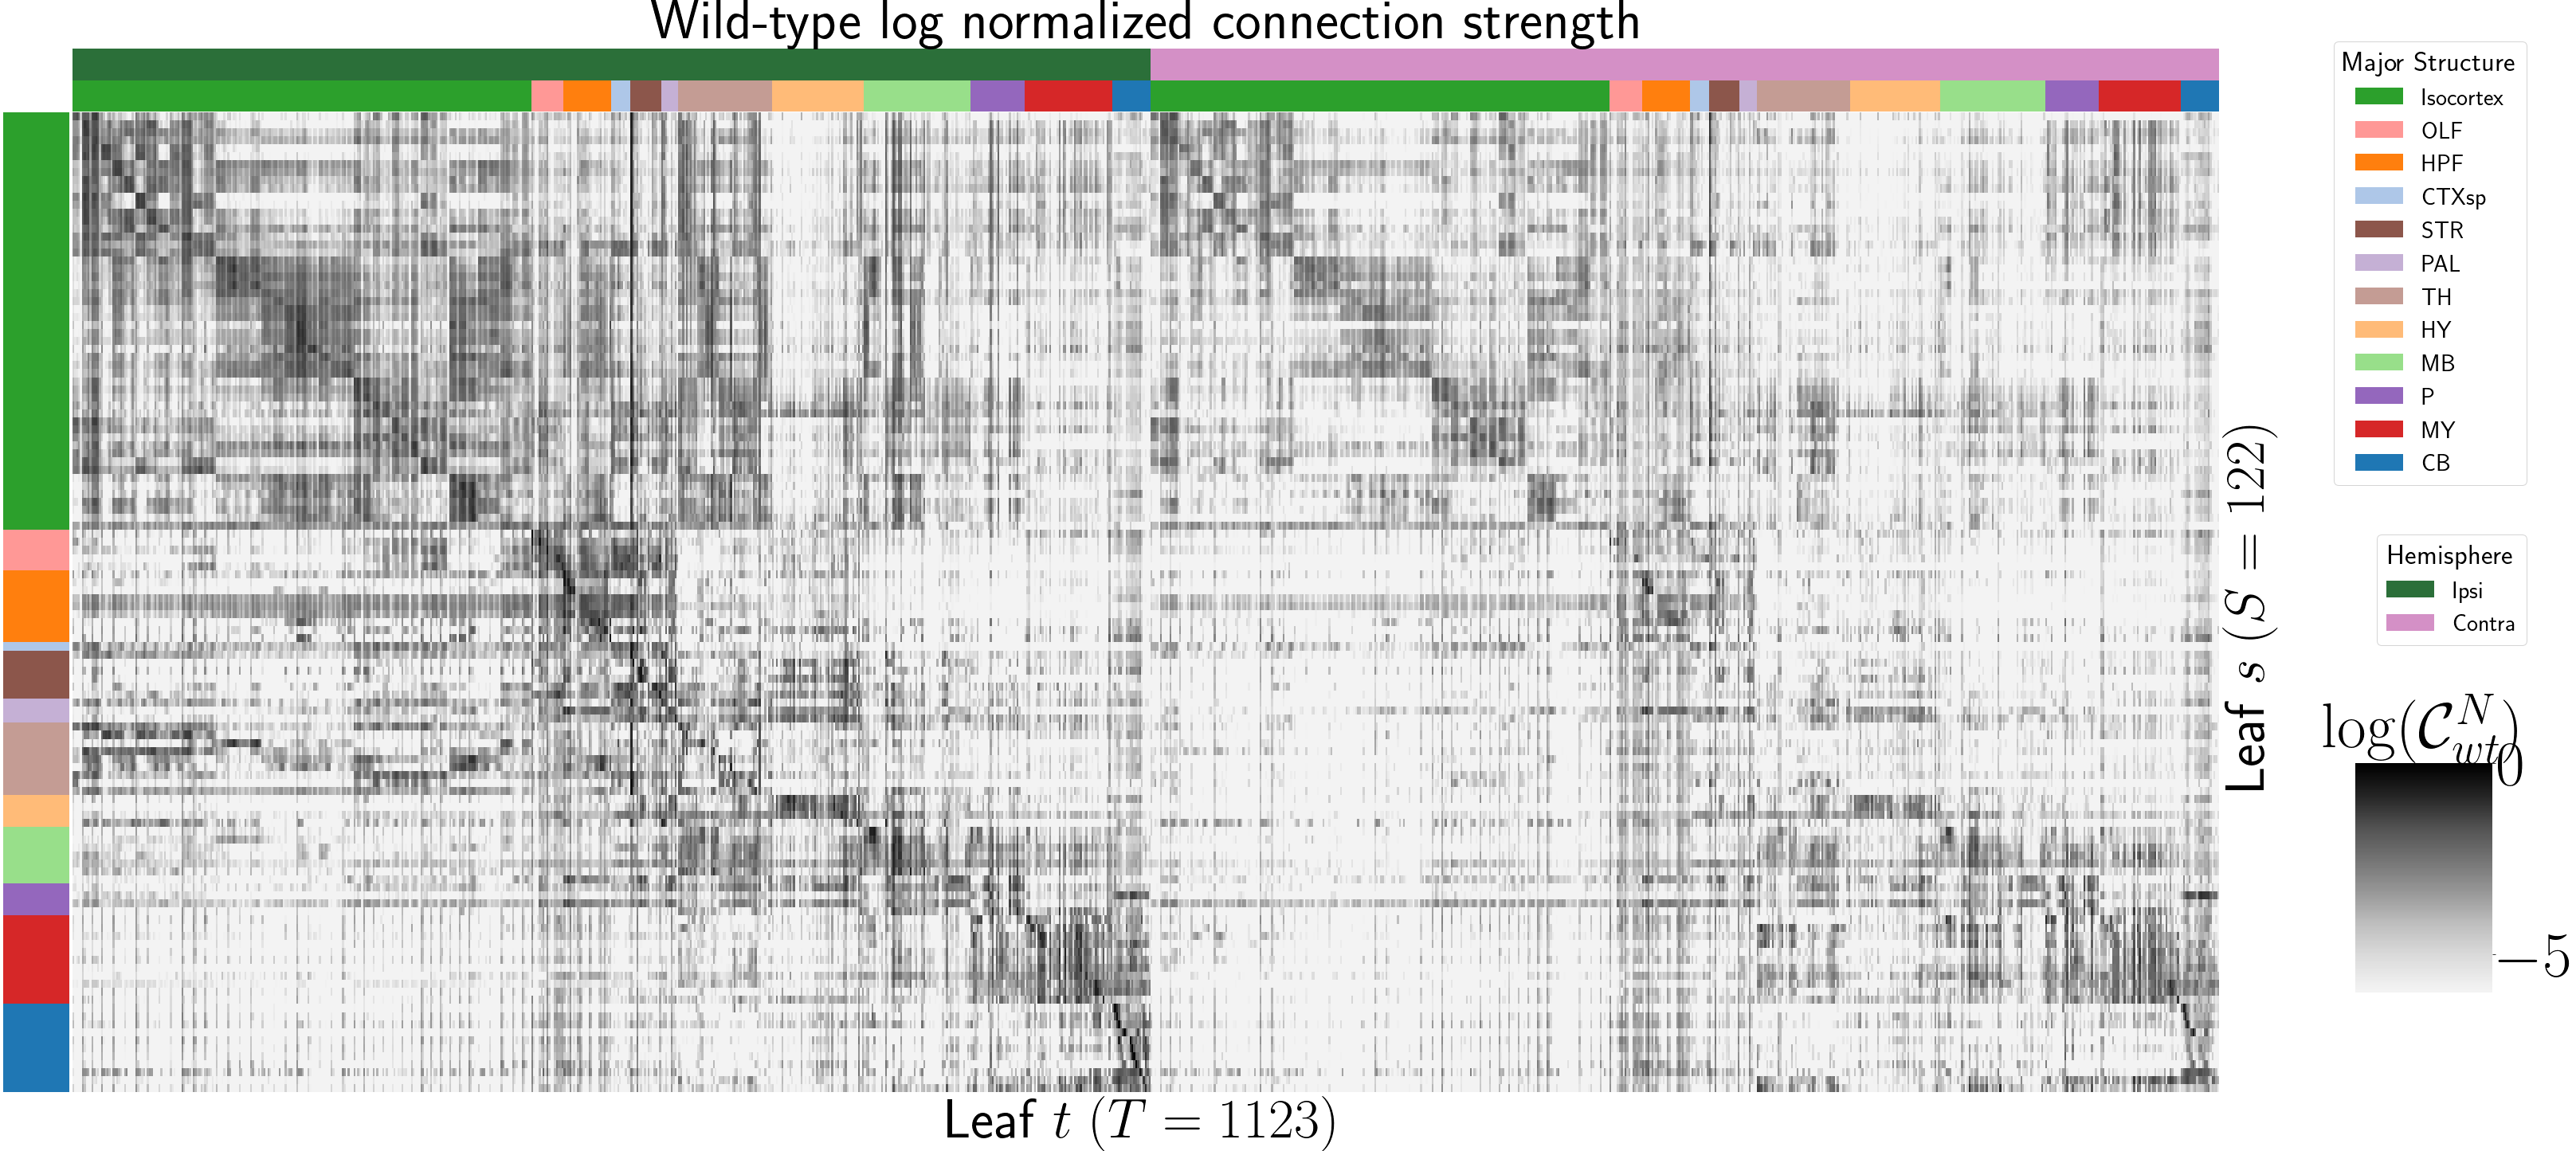
\includegraphics[width = \textwidth]{figs/conn_leaf2.png}
    } 
        \newline
       \subfloat[] {
    \label{fig:cortex_wt}
    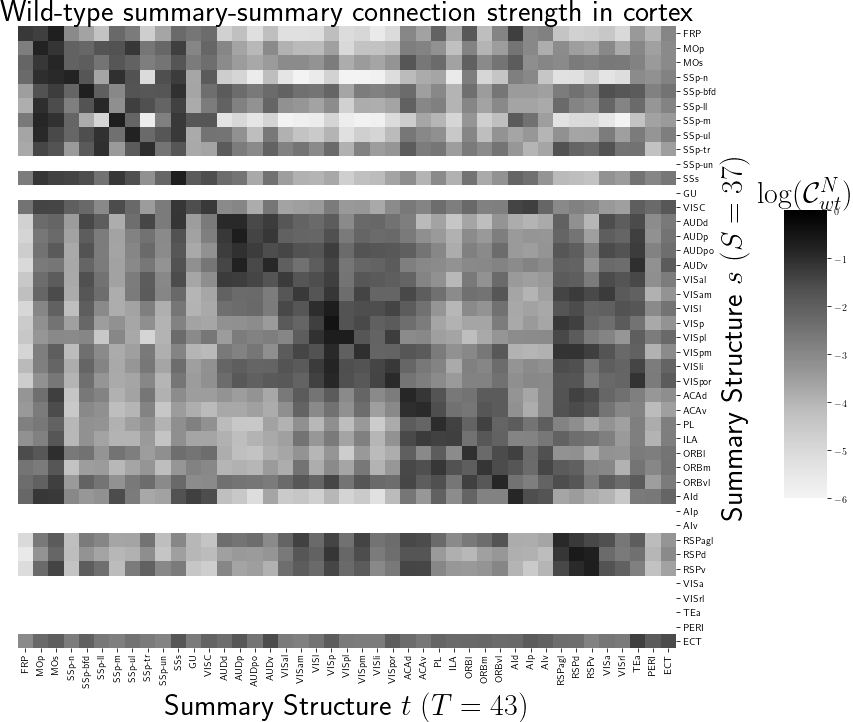
\includegraphics[width = .5\textwidth]{figs/conn_sum_cortex.png}
    } 
   \caption{Wild-type connectivities.
   \ref{fig:full_wt} Log wild-type connectivity matrix $\log \mathcal {C} (s,t,v_{wt})$.
   \ref{fig:cortex_wt} Log wild-type intracortical connectivity matrix at the summary structure level.}
   \label{fig:connectome}
\end{figure}

\newpage
\subsubsection{Class-specific connectivities}

Source and cell-type combinations which project similarly indicate the network structure underpinning cognition.
Our estimates of these class-specific connectivities exhibit certain known behaviors.
In Figure \ref{fig:data_ct}, we display results for the VISp and MO cortical areas.
These are ideal testbeds for our connectivities because they have well-established layer-specific projection patterns that can be detected with our layer-specific Cre-line based targeting \citet{Jeong2016-dc}, and are also well-represented in our dataset.

Our results are consistent with anterograde tracing experiments outside our dataset \citet{Jeong2016-dc}.
Figure \ref{fig:ct_spc} shows that in VISp, the Ntsr1-Cre line strongly targets the thalymic LP nuclei, and in MO, layer 5 projects to anterior basolateral amygdala (BLA) and capsular central amygdala (CEA), while layer 6 does not.
Recall that we display connectivity estimates for structures with at least one injection centroid in the structure.
Thus, the position of non-zero rows in Figure \ref{fig:ct_spc} shows the localization of Rbp4-Cre and Ntsr1-Cre injection centroids to layers 5 and 6 respectively (this is further examined in Supplemental Figure \ref{fig:iso_count}).
Thus, as a heuristic alternative model, to also synthesize information about leafs targeted by different Cre-lines, we also generate an average connectivity matrix over all Cre-lines.
This model is not evaluated in our testing, and is only a general stand-in for overall behavior, but provides a useful summary of results.

Cell-class, while often correlated with cortical layer, is often a stronger driver of connectivity than summary structure.
Figure \ref{fig:ct_clust} shows a collection of connectivity strengths generated using cre-specific models for wild-type, Cux2, Ntsr1, Rbp4, and Tlx3 cre-lines from visual signal processing leafs in the cortex to cortical and thalymic nucleii.
We use heirarchical clustering to sort source structure/cell-class combinations by the similarity of their structural projections, and sort target structures by the structures from which they receive projections.
Examining the former, we can see that the Ntsr1 Cre-line distinctly projects to thalymic nucleii, regardless of summary structure.
This contrasts with the tendency of other cell-classes to project intracortically in a manner determined by the source structure.
Similarly, layer 6 targets are not strongly projected to by any of the displayed Cre-lines.
There are too many targeted summary structures to plot here, but we expect that the source profile of each target clusters by structure.

\newpage

\begin{figure}[H]
\subfloat[]{
\label{fig:ct_spc}
    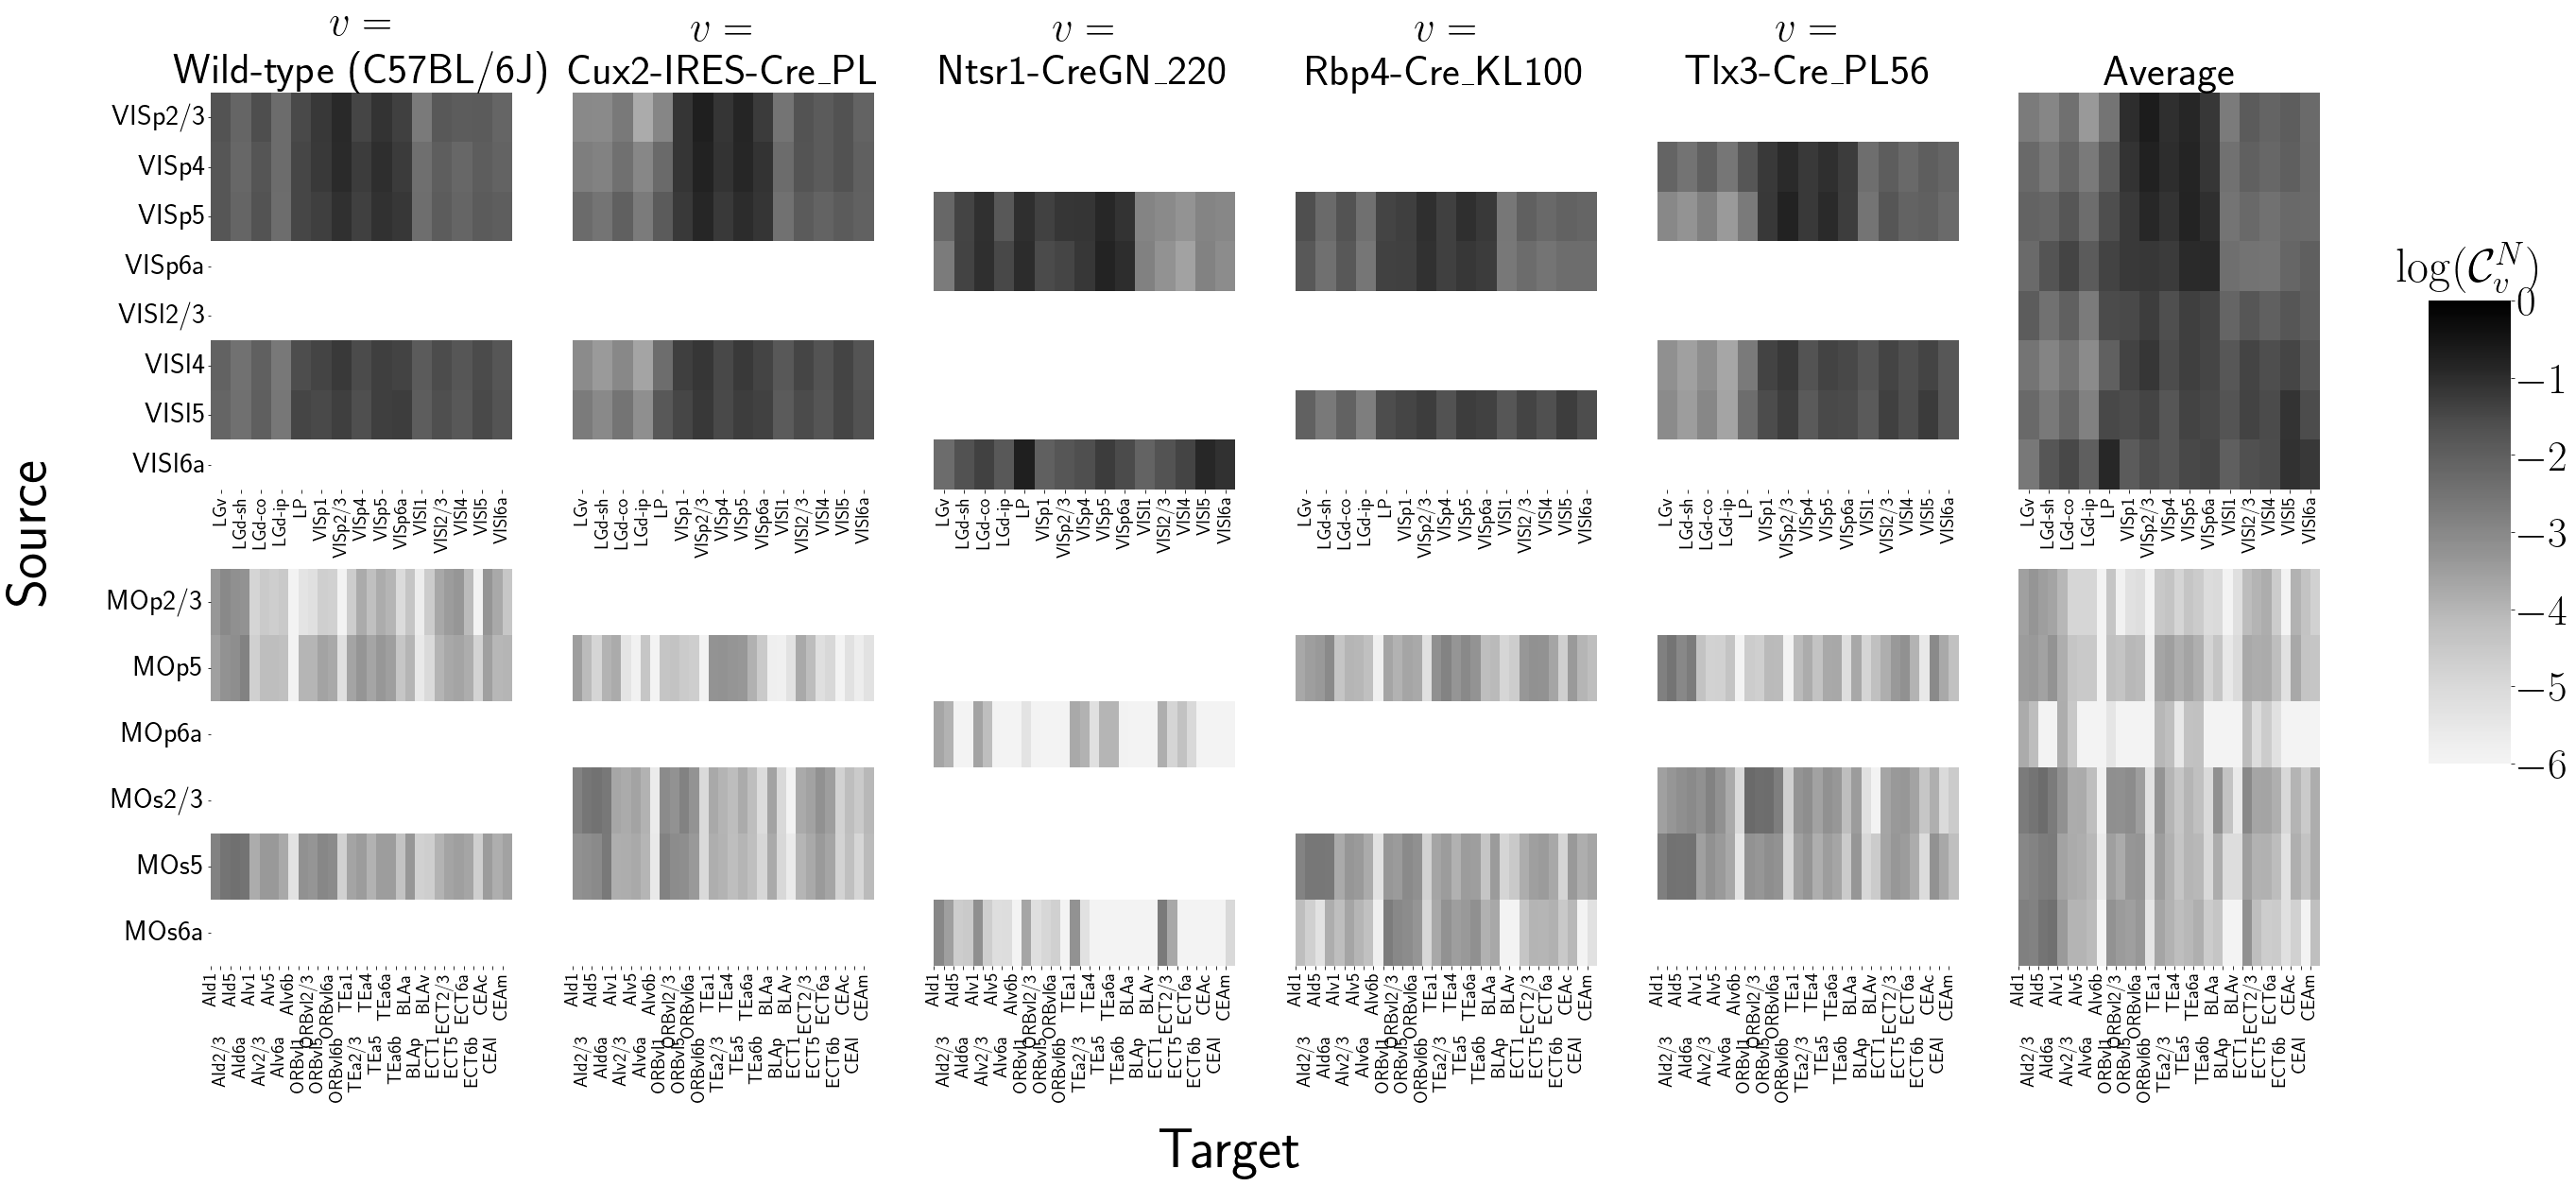
\includegraphics[width=.8\textwidth]{figs/visp_mo.png} 
    }
    \newline
 \subfloat[]{
 \label{fig:ct_clust}
    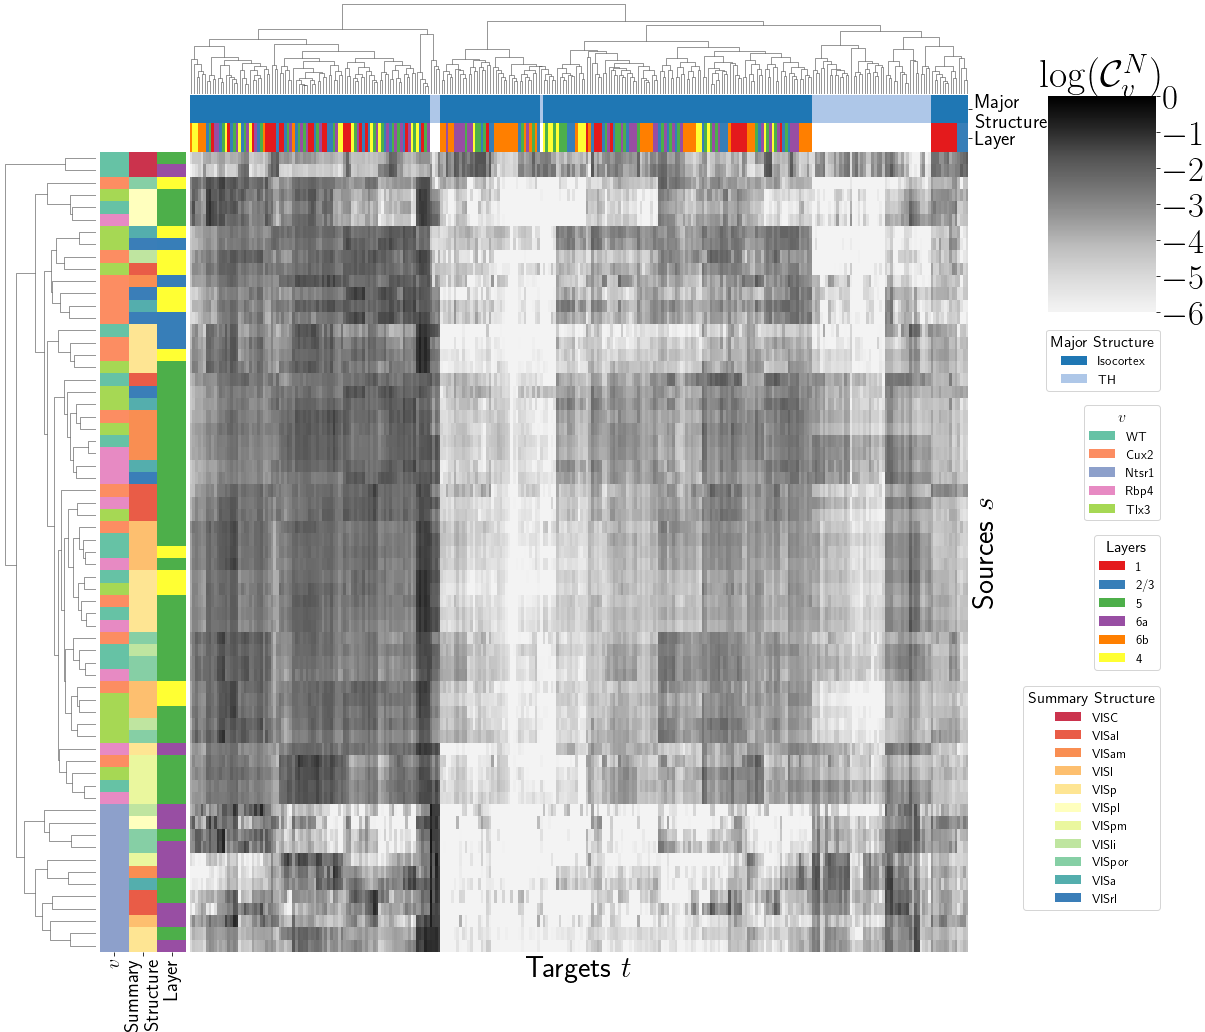
\includegraphics[width=.6\textwidth]{figs/heirarchical.png}
    }
    
    \caption{  Cell-class specificity. \ref{fig:ct_spc} Selected cell-class and layer specific connectivities from VISp and MO.
	 Sources without a injection of that Cre-type are not estimated due to lack of data for that Cre-line in that structure.
    		\ref{fig:ct_clust}
		Heirarchical clustering of connectivity strengths from visual signal processing cell-types to cortical and thalymic targets.
		Cre-line, summary structure, and layer are labelled on the sources.
		Major brain division and layer are labelled on the targets.}
\label{fig:data_ct}
\end{figure}

\newpage

\subsection{Connectivity Analyses}

Each structural connectivity matrix is a high-dimensional realization of relatively few biological processes, and decomposition of neural signals to recover these processes is a fundamental goal in neuroscience.
In this section, we apply non-negative matrix factorization to decompose the long-range wild-type connectivities into linear combinations of archetypal connectivities.
This decomposes the remaining censored connectivity matrix into a linear model based off a relatively small number of distinct signals.
This model is able to capture a large amount of the observed variability, and recovers structure-specific archetypal signals.

These signals are plotted in Figure \ref{fig:nmf_results}, and technical details and intermediate results are given in Supplemental Sections \ref{supp_sec:matrix_factor_methods} and \ref{supp_sec:matrix_factor_results}, respectively.
These details include a cross-validation based method for selecting the number of components, a masking method for focusing only on long range connections, and a stability method for ensuring that the decomposition is reliable across computational replicates.
The plotted decomposition shows that these underlying connectivity archetypes correspond strongly to major brain division.
However, certain components that predominantly represent connectivity from a given major brain division may also be accessed from other areas.
For example, the IP and FN regions of CB are strongly associated in \ref{fig:W} with the component projecting to MY in \ref{fig:H}.

Inspection of the reconstructed distal normalized connection strength using the top $15$ components shows qualitatively shows that this relatively sparse decomposition is able to capture much of the observed variability.
Layer-specific targeting is evident, indicating that the factorization method is detecting cell-type specific signals, even though it is trained only on the wild-type connectivity.
Other connectivity patterns like cortical-cortical and cortical-thalymic are also detected.

\newpage

\begin{figure}[H]
\centering
\hspace{1cm}
\subfloat[]{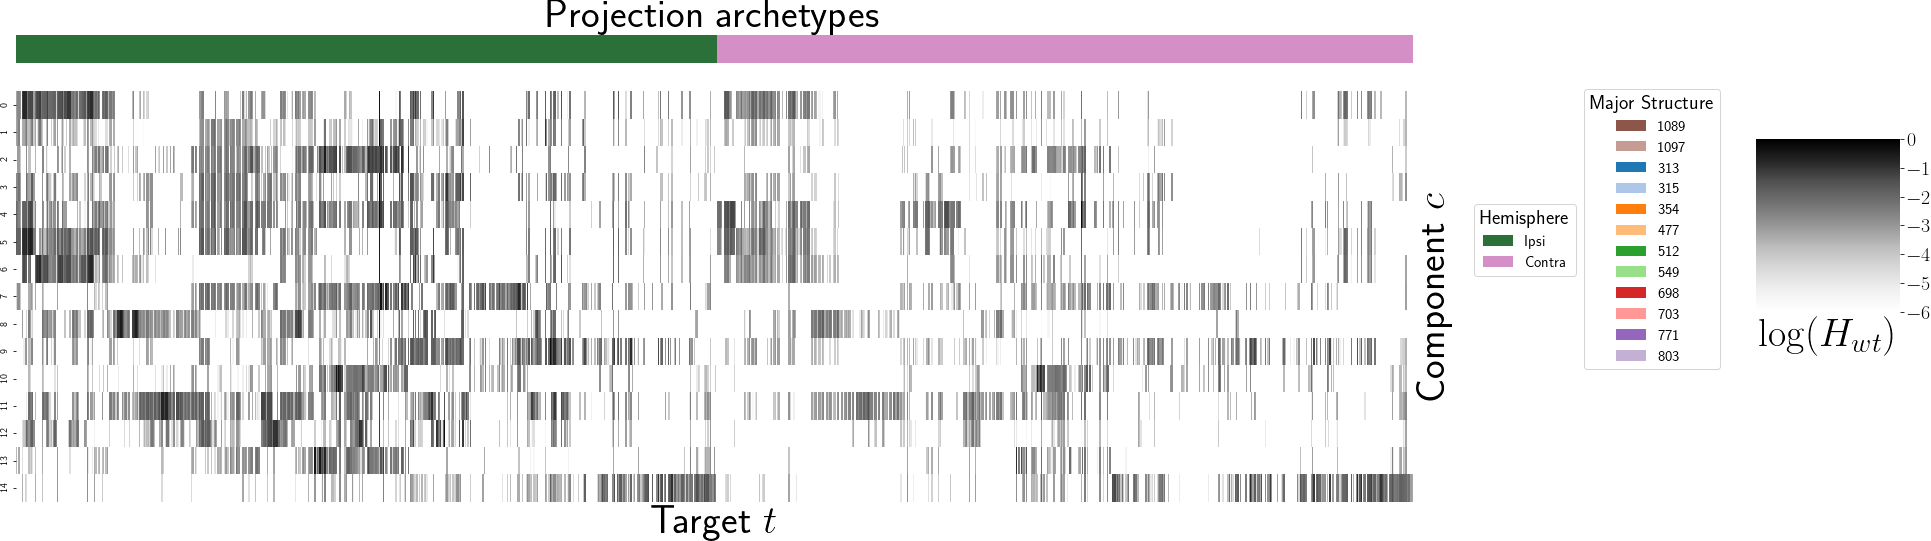
\includegraphics[width = .85 \textwidth]{figs/H_wt.png}
\label{fig:H}} 
\newline
\begin{tabular}[t]{cc}
\adjustbox{valign=t}{\subfloat[]{
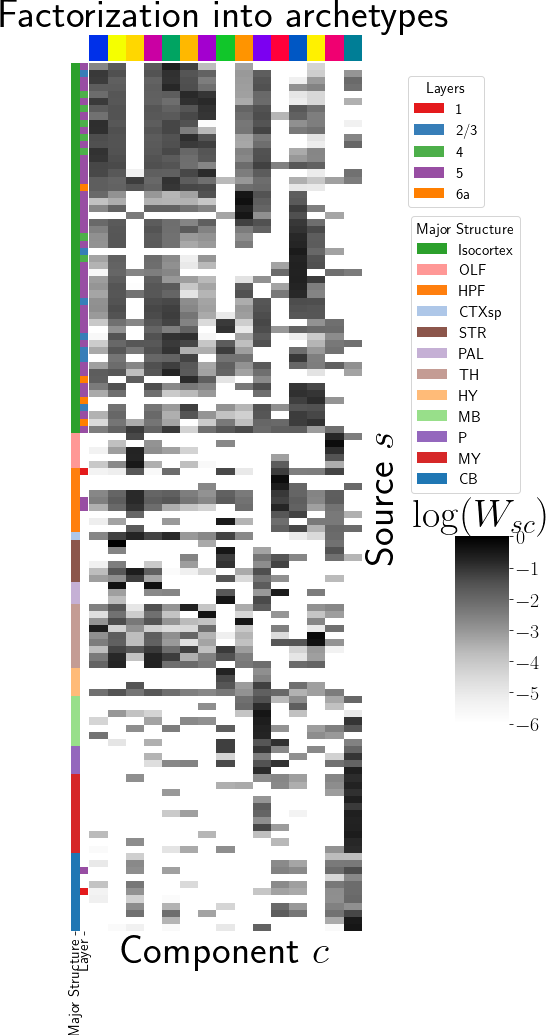
\includegraphics[width = .3\textwidth]{figs/W_wt.png}
\label{fig:W}}
} & 
\adjustbox{valign=t}{\subfloat[]{
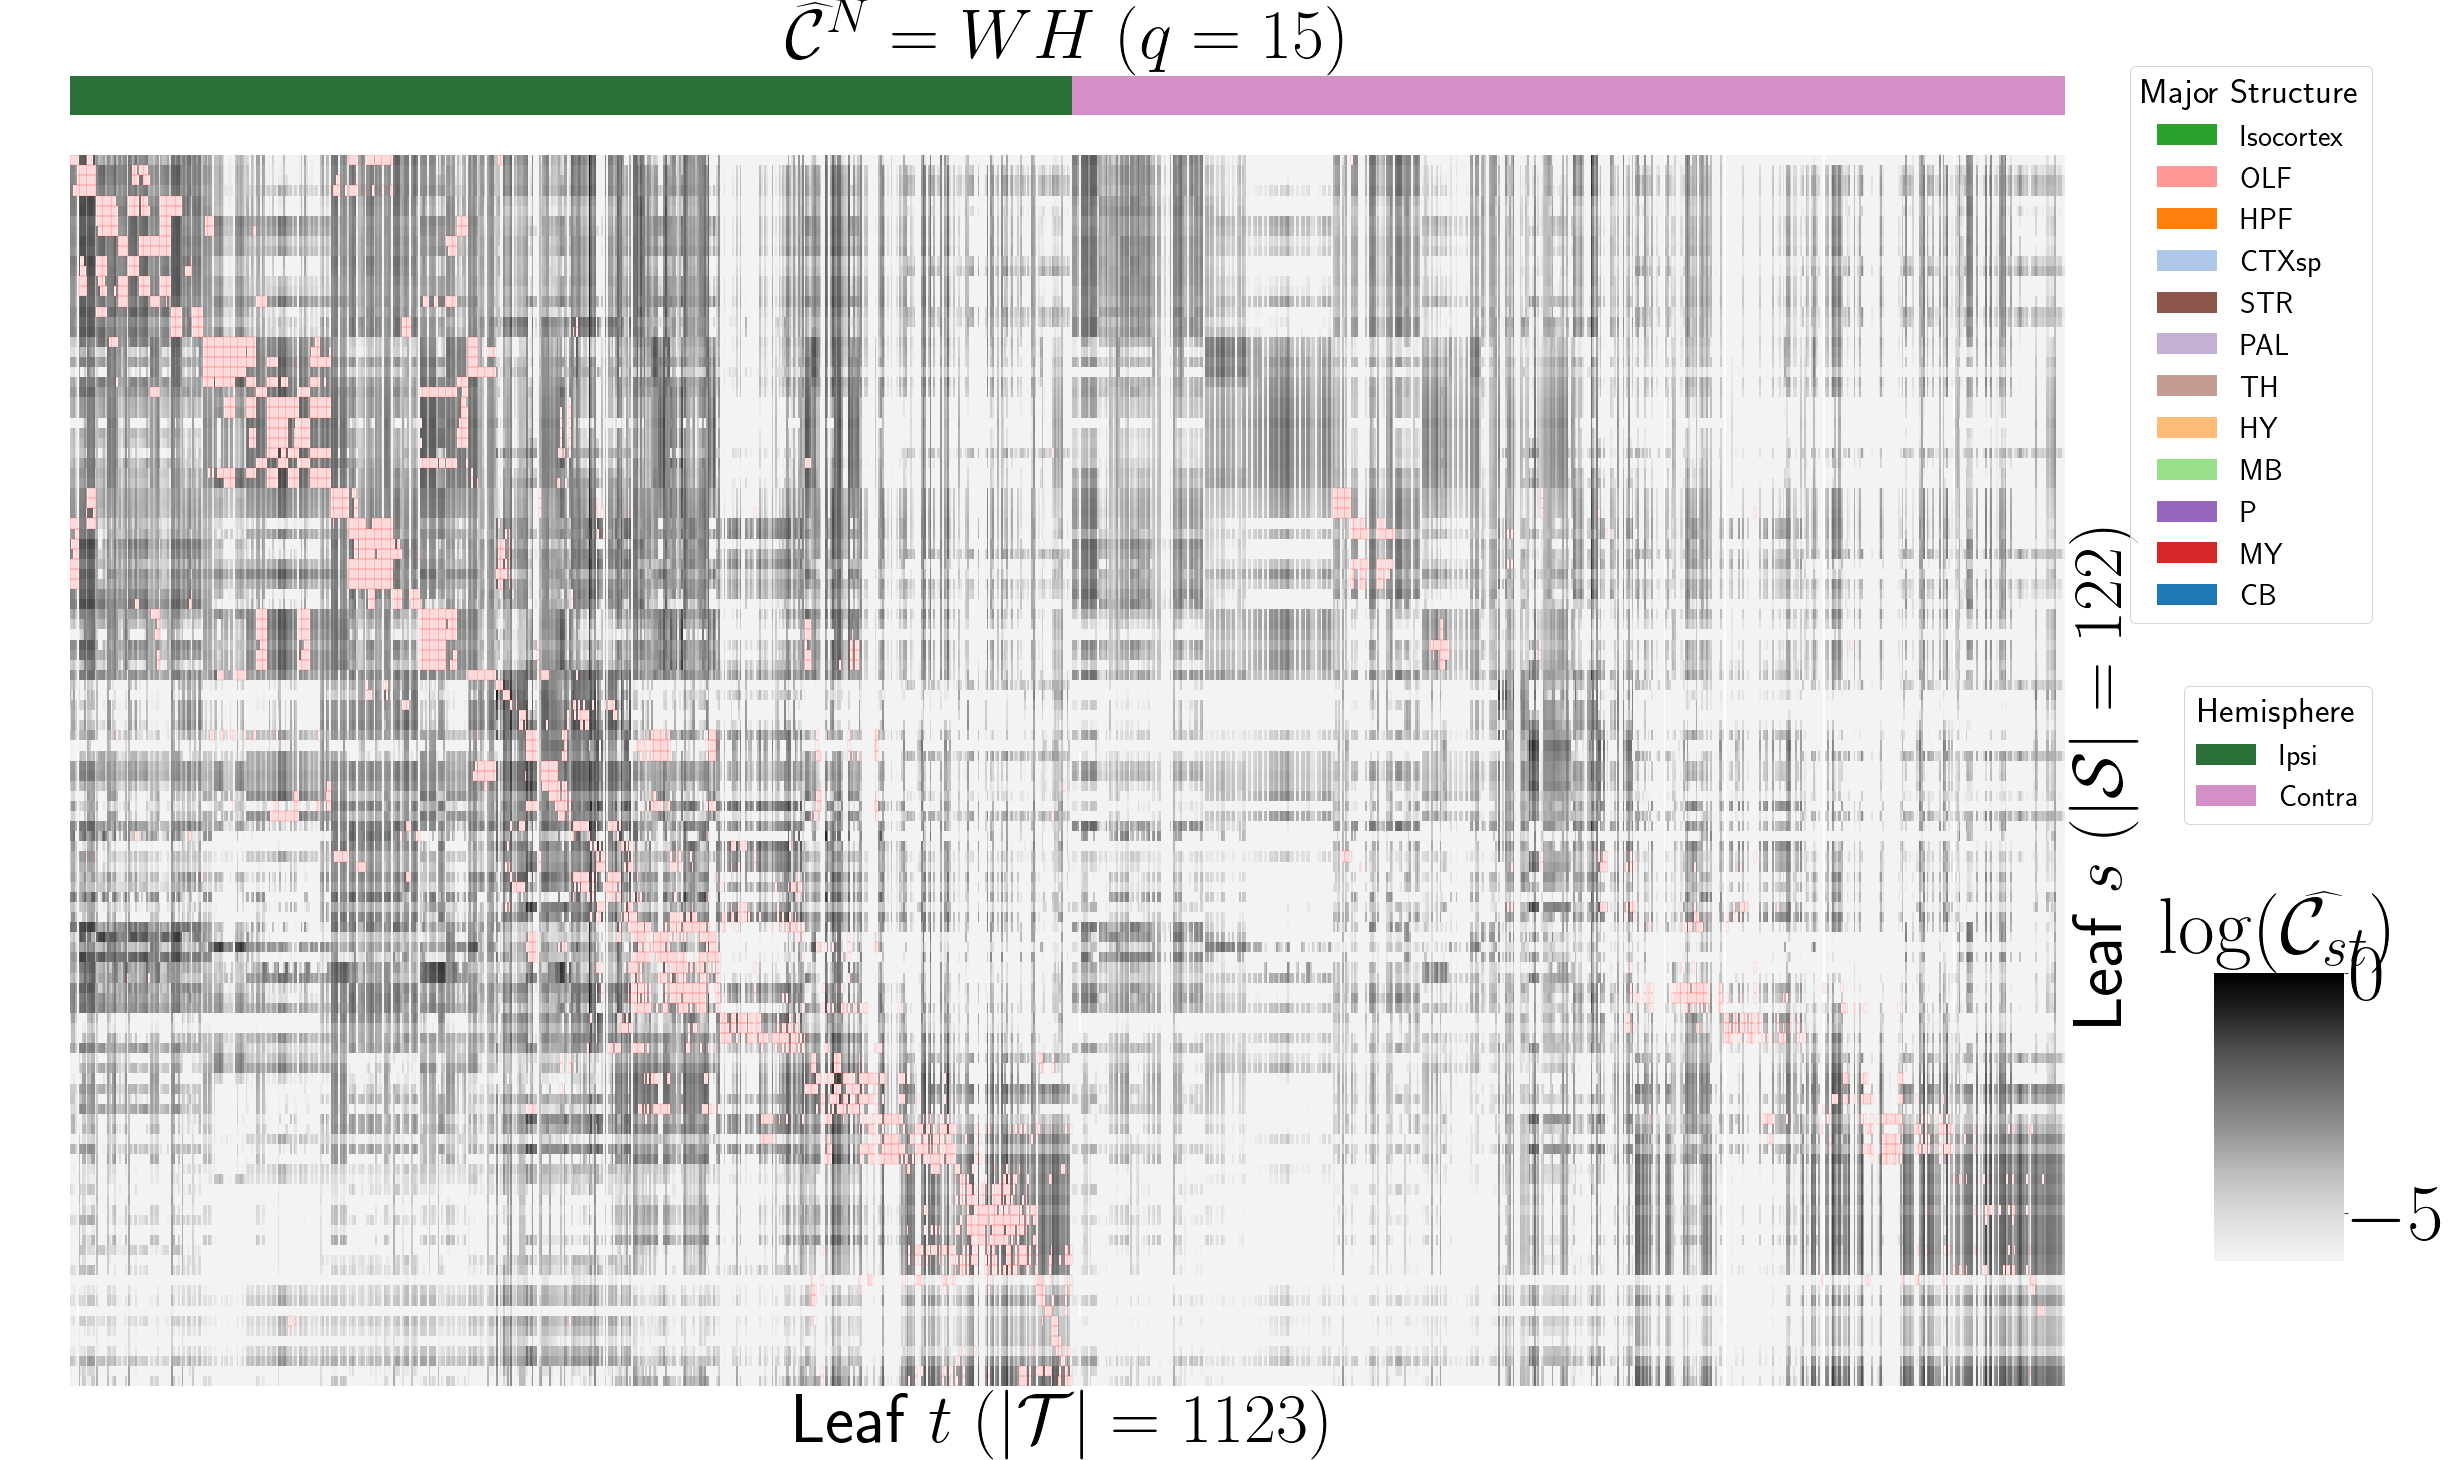
\includegraphics[width = .7\textwidth]{figs/conn_leafs_recon.png}
\label{fig:recon}}
} 
\end{tabular}
\caption{Non-negative matrix factorization results $\mathcal C_{wt}^N = WH$ for $q = 15$ components.
\ref{fig:H} Latent space coordinates $H$ of $\mathcal C$.
Target major structure and hemisphere are plotted.
\ref{fig:W} Loading matrix $W$.
Source major structure and layer are plotted.
\ref{fig:recon} Reconstruction of the normalized distal connectivity strength using the top $15$ archetypes.  Areas less than $1500 \mu m$ apart are not modeled, and therefore shown in red.
}
\label{fig:nmf_results}
\end{figure}

\newpage


\newpage
\section{Discussion}

We see several opportunities for improving on our model.
Our particular task of transforming the injection and projection signal depending on cell-type is a non-linear transformation problem with categorical covariate.
Model averaging based off of cross-validation has been implemented in \citet{Gao2016-qe}, but we note that our approach makes use of a non-parametric estimator, rather than an optimization method for selecting the weights \citep{Saul2003-th}, and is applied specifically to a target-encoded feature space.
The properties of this estimator, as well as its relation to estimators fit using an optimization algorithm, are a possible future avenue of research.
Therefore, a deep model such as \citet{Lotfollahi2019-tr} could be appropriate, provided enough data was available.
With respect to the model, a Wasserstein-based measure of injection similarity per structure would combine both the physical simplicity of the centroid model while also incorporating structural knowledge.
Residual models of the above could also be considered.

The factorization of the connectivity matrix could be similarly improved.
Flattening $\mathcal C$ prior to unsupervised analysis is not necessarily recommended, but provides an easy solution for this problem.


%The Nadaraya-Watson weighting procedure introduced here is, to our knowledge, novel. 

%We make a key assumption: that the additional statistical accuracy of including more samples makes up for the fact that their expected accuracy is lower.
%Note that this assumption can be easily violated, if, for example, the data is distributed on a circle without error, and only nearest neighbors are most predictive.


%\skcomment{CITE METHOD THAT SELECTS WEIGHTS IN KERNEL (has catchy name)}


%The major-structure specific Nadaraya-Watson estimator from $\citet{Knox2019-ot}$ nevertheless appears poorly adapted for our circumstances since it does not take into account the virus $v$. It is not straightforward to include the viral strain in either $f_{NW}$ or $f_{NNLS}$. For $f_{NW}$, it is not clear how a one-hot encoded class-membership feature should be weighted. For $f_{NNLS}$, our sample size seems too low to utilize a fixed or mixed effect, particularly since the impact of the virus depend on the particular injection region, motivating use of an interaction term.


%%%%%%%%%%%%%%%%%%%%%%%%%%%%%%%%%%%%%%%%%%%%%%%%%%%%%%%%%%%%%%%%%
%%% End of Article

% \acknowledgments
% \section{Supporting Information} (optional)
% \section{Competing Interests} (optional)
% \bibliography{<name of .bib file>}




\newpage

\acknowledgments
We thank the Allen Institute for Brain Science founder, Paul G. Allen, for his vision, encouragement, and support.
\newpage
This supplement is divided into information about our dataset, supplemental methods, and supplemental results.
However, certain topics are revisited between sections.
Thus, if a reader is interested in, say, non-negative matrix factorization, they may find relevant information in both methods and results.

\section{Supplemental Information}
\label{supp_sec:info}

Our supplementary information consists of abundances of leaf/Cre-line combinations, information about distances between structures, and the size of our restricted evaluation dataset.

\subsection{Cre/structure combinations in $\mathcal D$}
\label{supp_sec:data}

This section describes the abundances of leaf and Cre-line combinations in our dataset.
Users of the connectivity matrices who are interested in a particular Cre-line or structure can see the quantity and type of data used to compute and evaluate that connectivity.

\newpage

\begin{figure}[H]
    \centering
    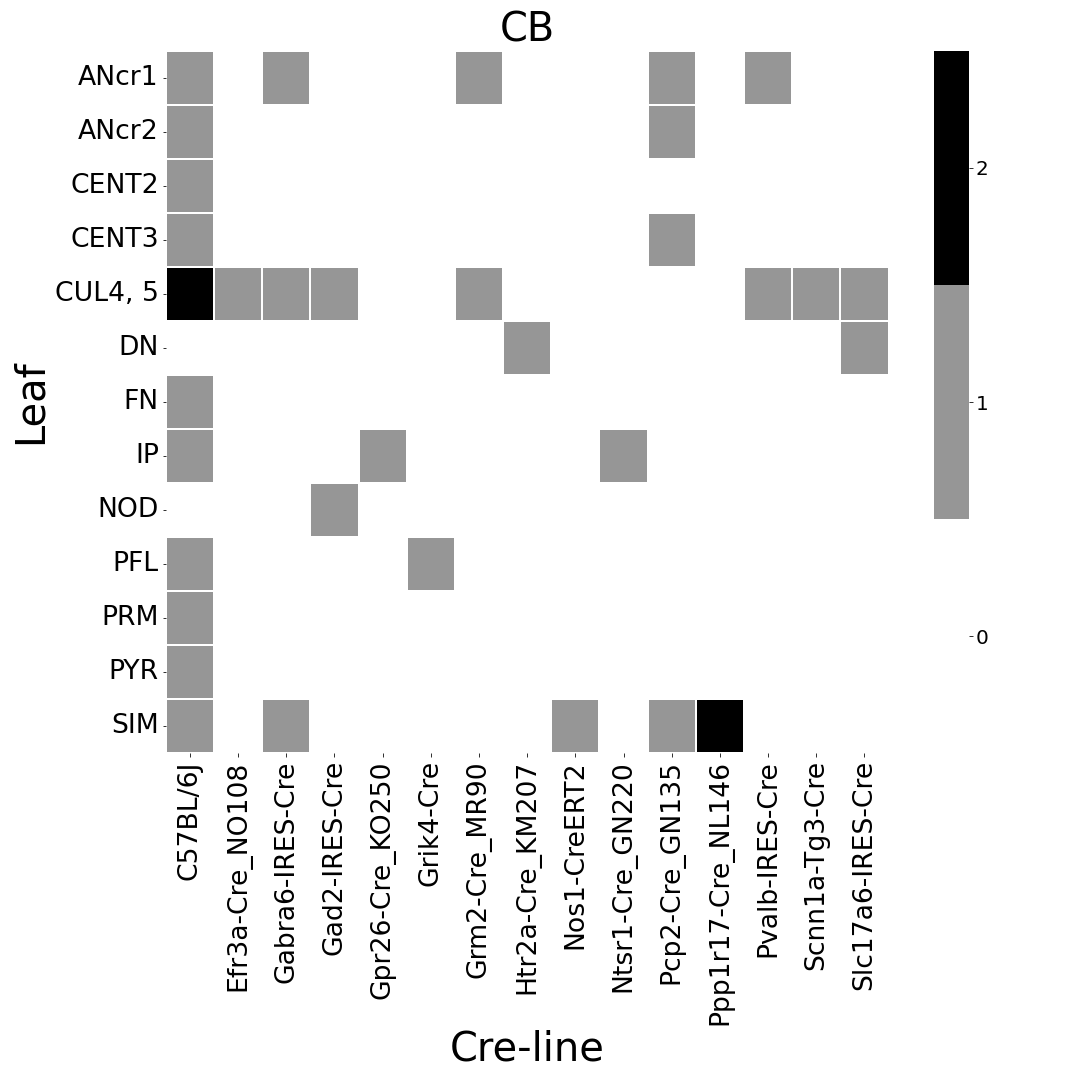
\includegraphics[width = 7in]{figs/CB centroid density.png}
    \label{fig:my_label}
\end{figure}
\newpage

\begin{figure}[H]
    \centering
    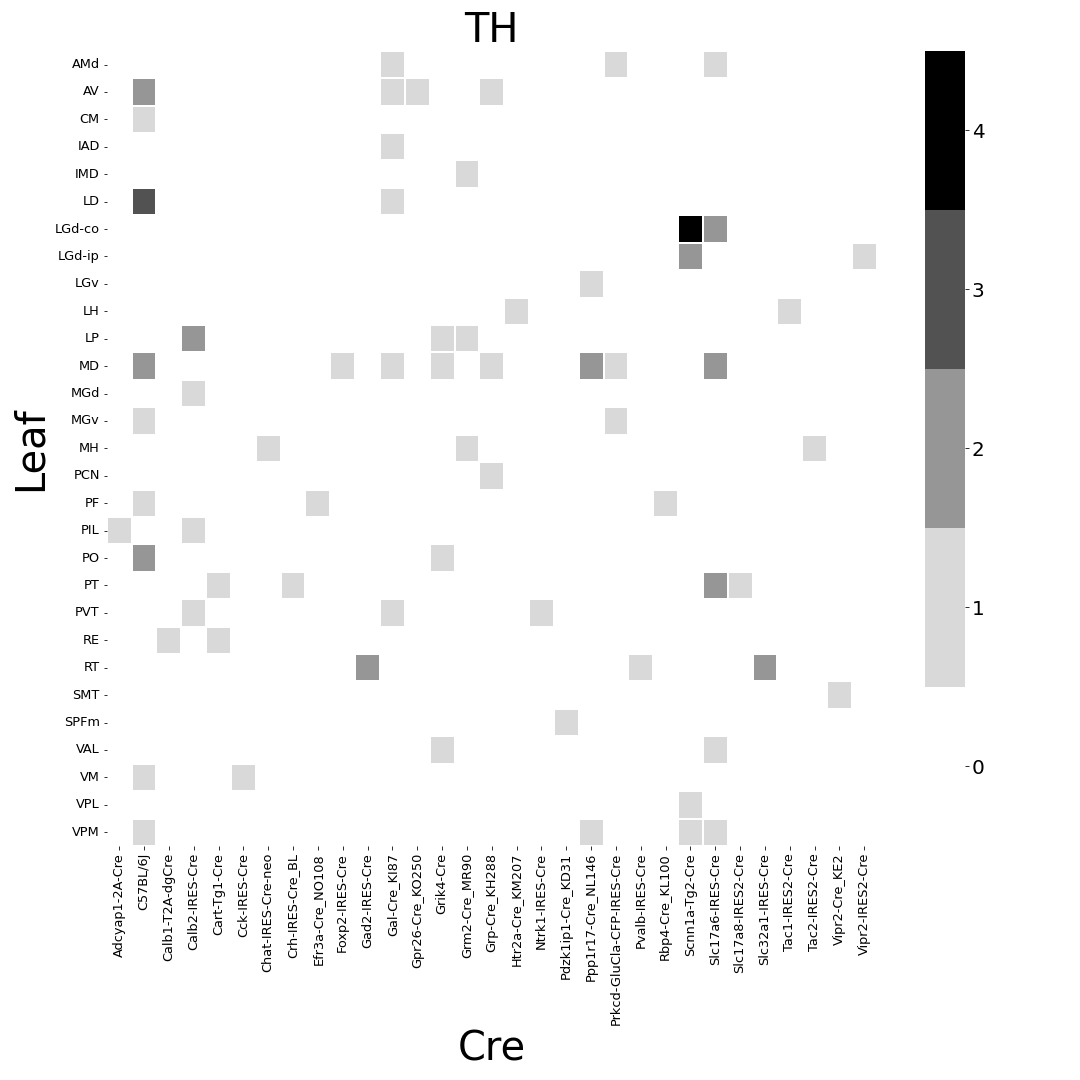
\includegraphics[width = 7in]{figs/TH centroid density.png}
    \caption{Caption}
    \label{fig:my_label}
\end{figure}
\newpage

\begin{figure}[H]
    \centering
    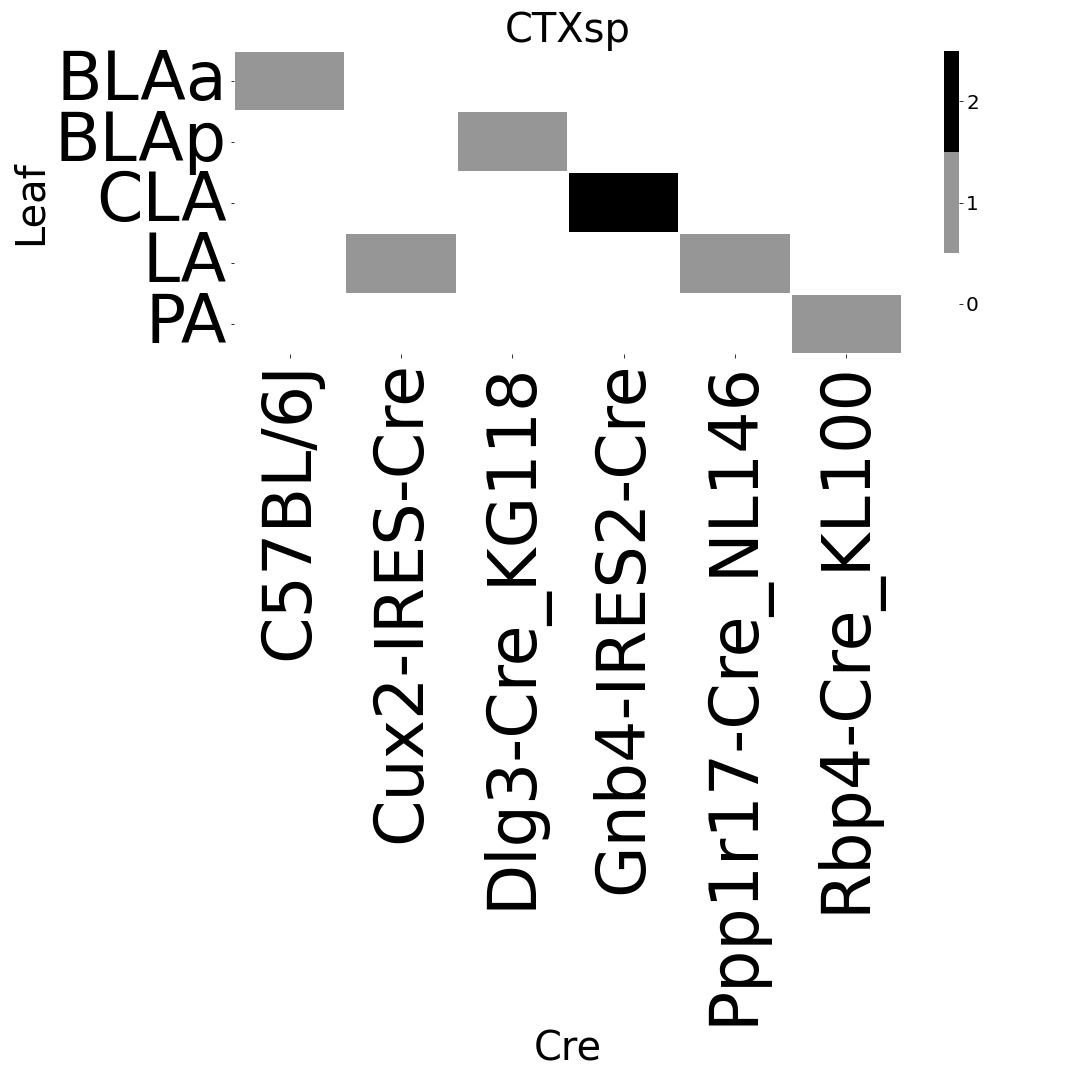
\includegraphics[width = 7in]{figs/CTXsp centroid density.png}
    \caption{Caption}
    \label{fig:my_label}
\end{figure}
\newpage

\begin{figure}[H]
    \centering
    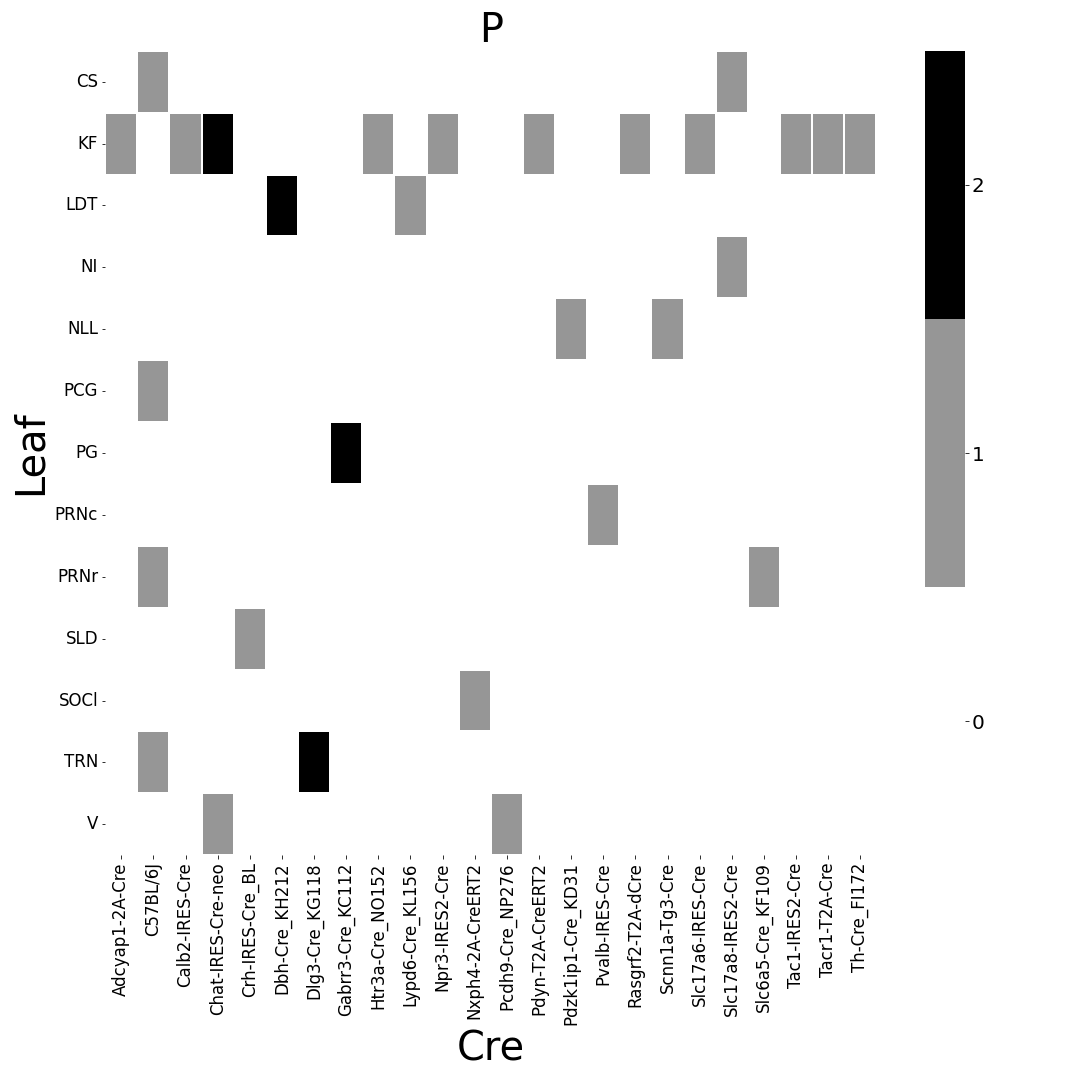
\includegraphics[width = 7in]{figs/P centroid density.png}
    \label{fig:my_label}
\end{figure}
\newpage

\begin{figure}[H]
    \centering
    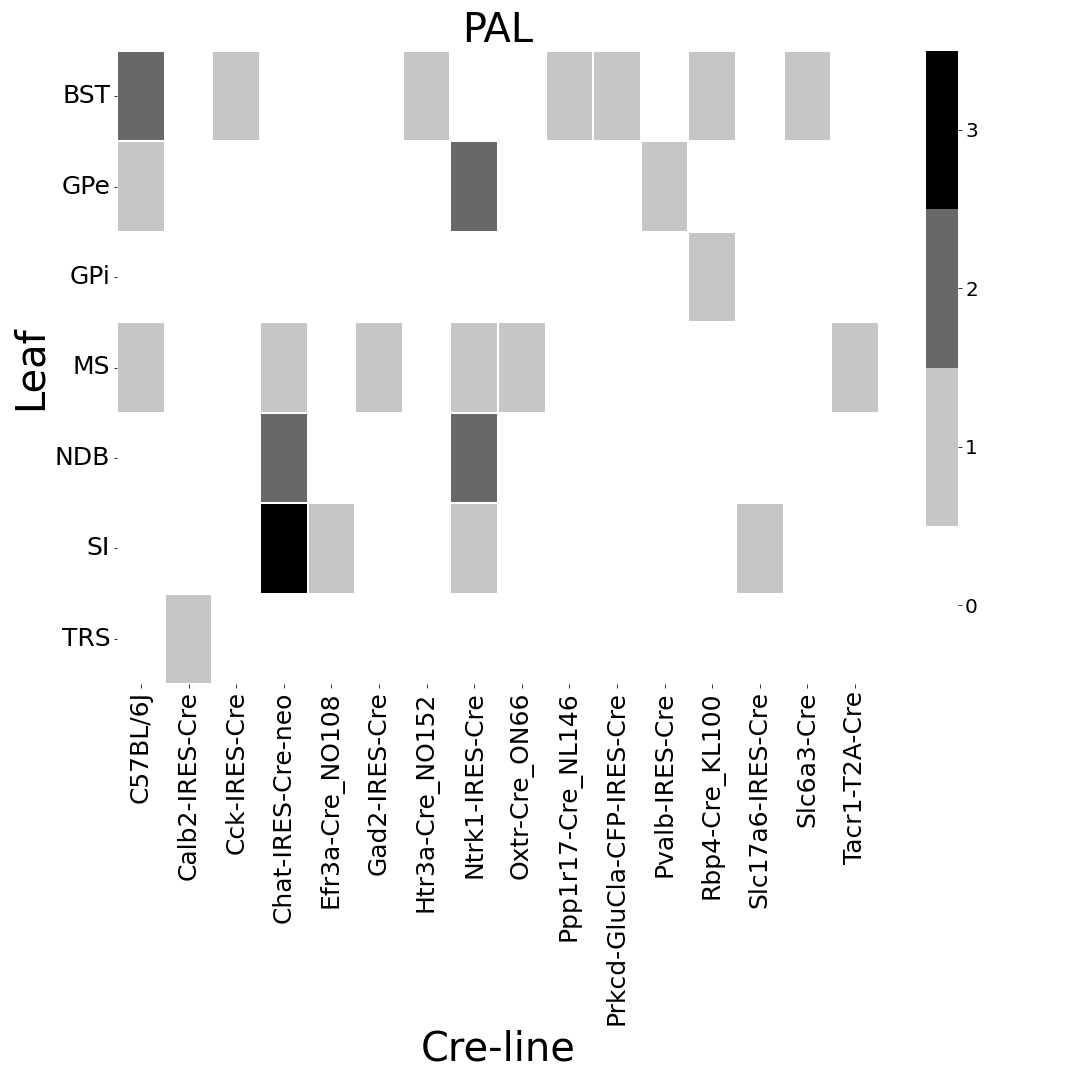
\includegraphics[width = 7in]{figs/PAL centroid density.png} 
    \label{fig:my_label}
\end{figure}
\newpage

\begin{figure}[H]
    \centering
    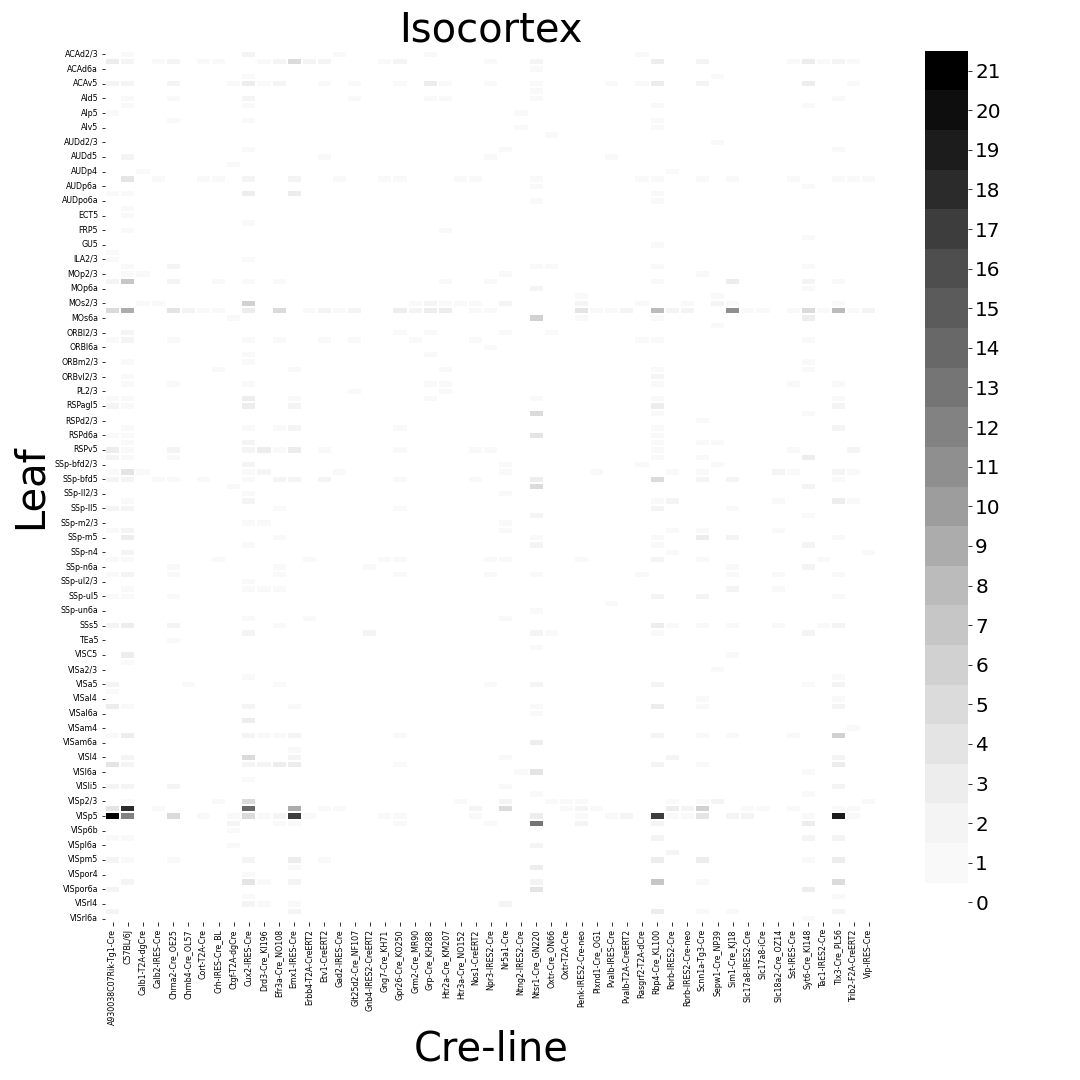
\includegraphics[width = 7in]{figs/Isocortex centroid density.png}
    \label{fig:iso_count}
\end{figure}
\newpage

\begin{figure}[H]
    \centering
    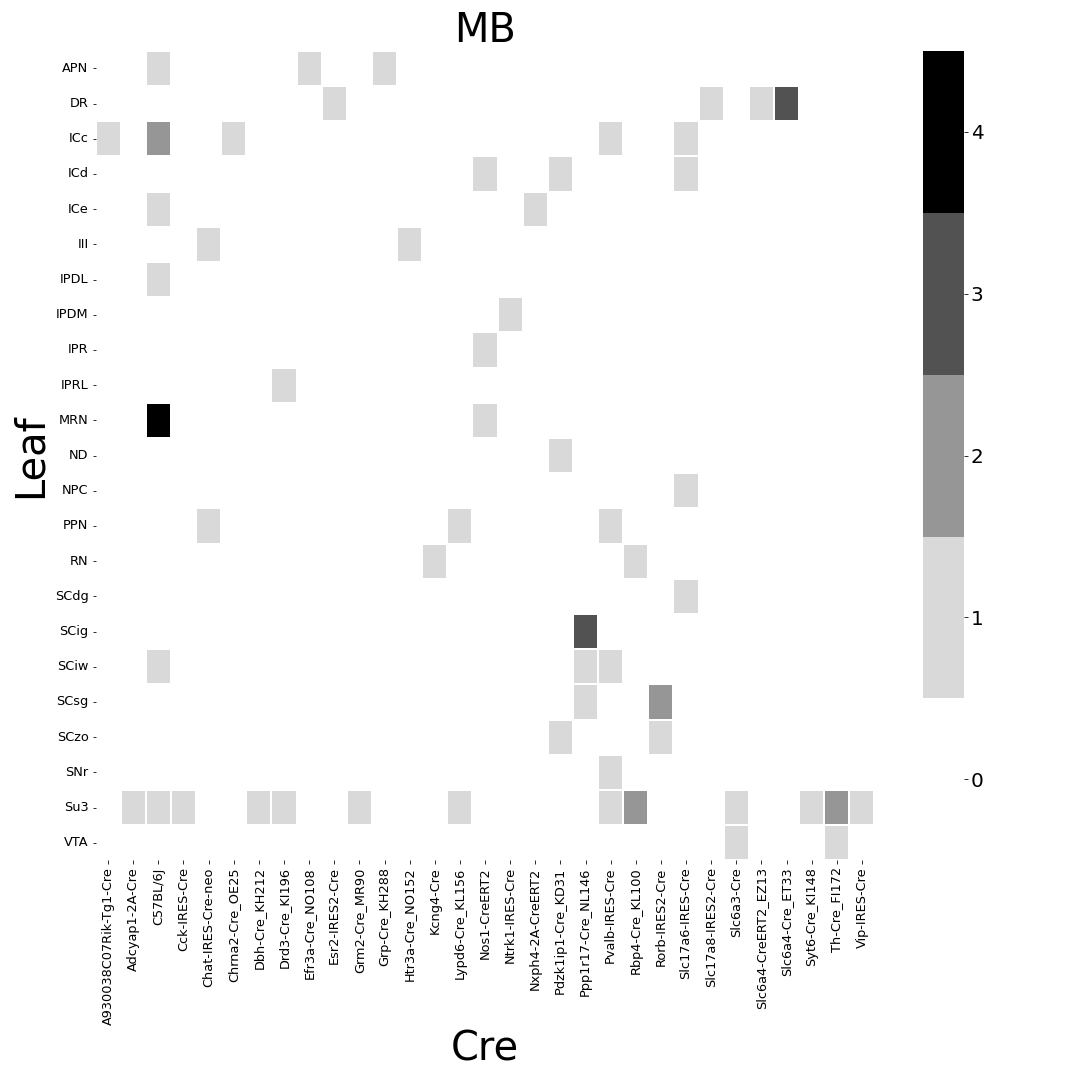
\includegraphics[width = 7in]{figs/MB centroid density.png} 
    \label{fig:my_label}
\end{figure}
\newpage

\begin{figure}[H]
    \centering
    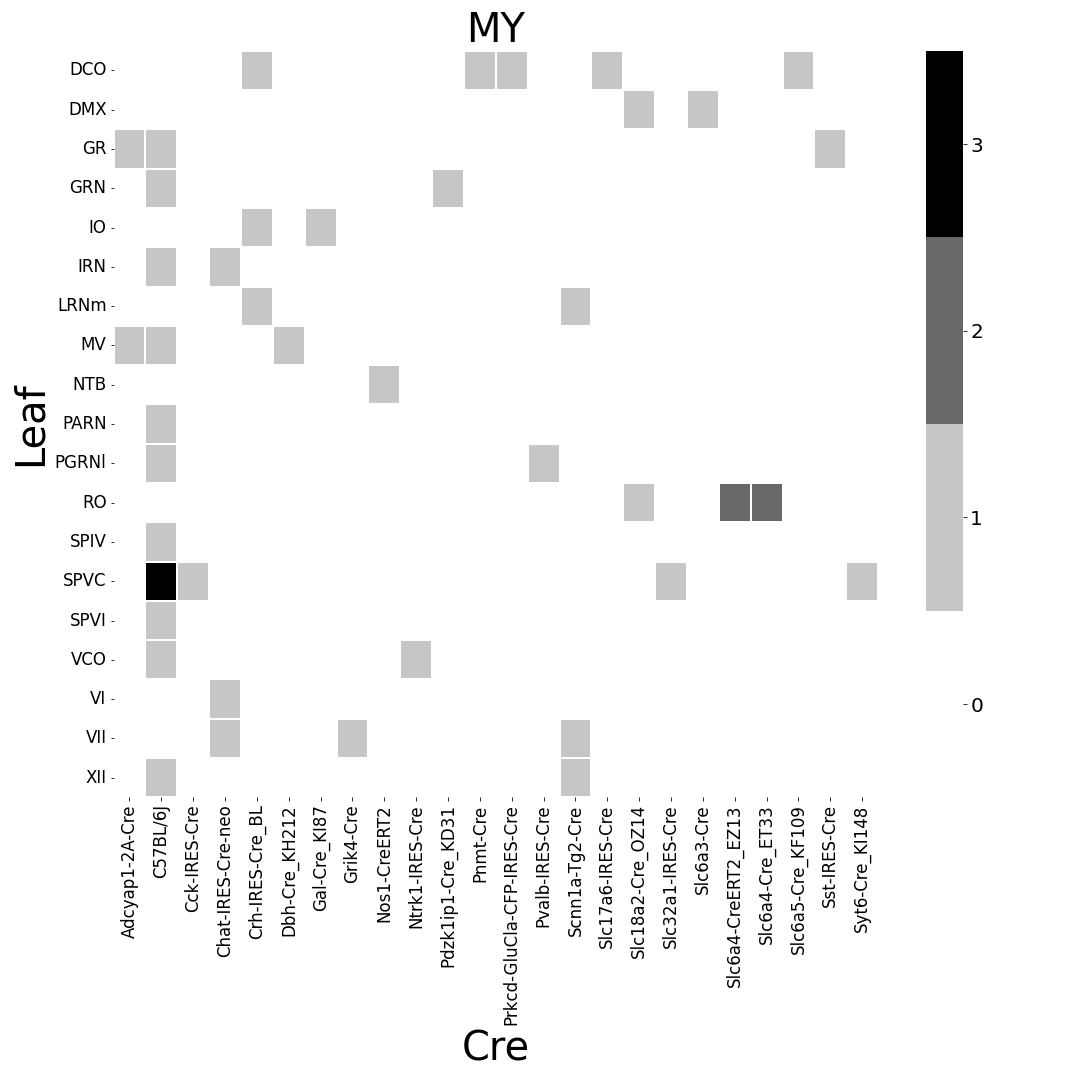
\includegraphics[width = 7in]{figs/MY centroid density.png} 
    \label{fig:my_label}
\end{figure}
\newpage

\begin{figure}[H]
    \centering
    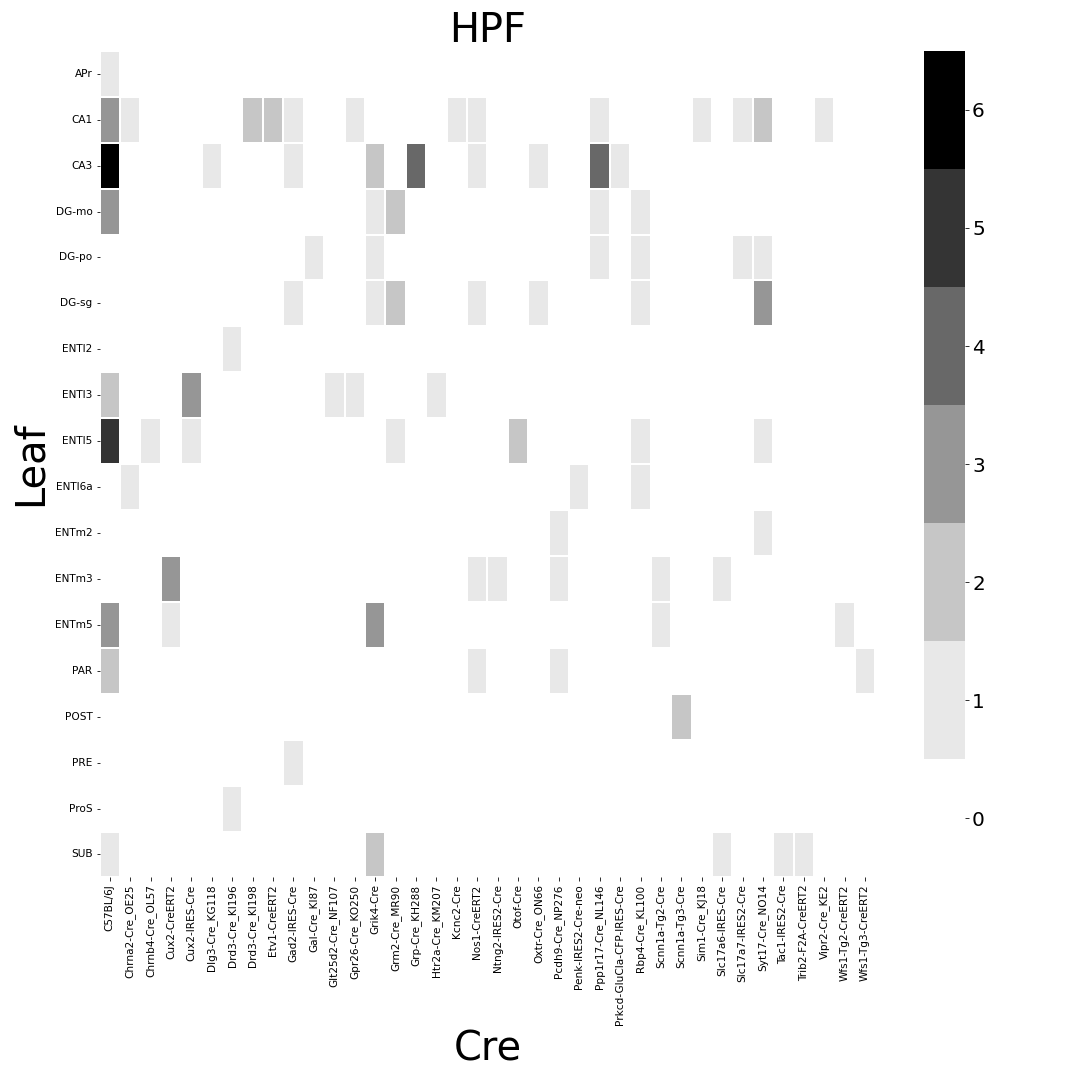
\includegraphics[width = 7in]{figs/HPF centroid density.png} 
    \label{fig:my_label}
\end{figure}
\newpage

\begin{figure}[H]
    \centering
    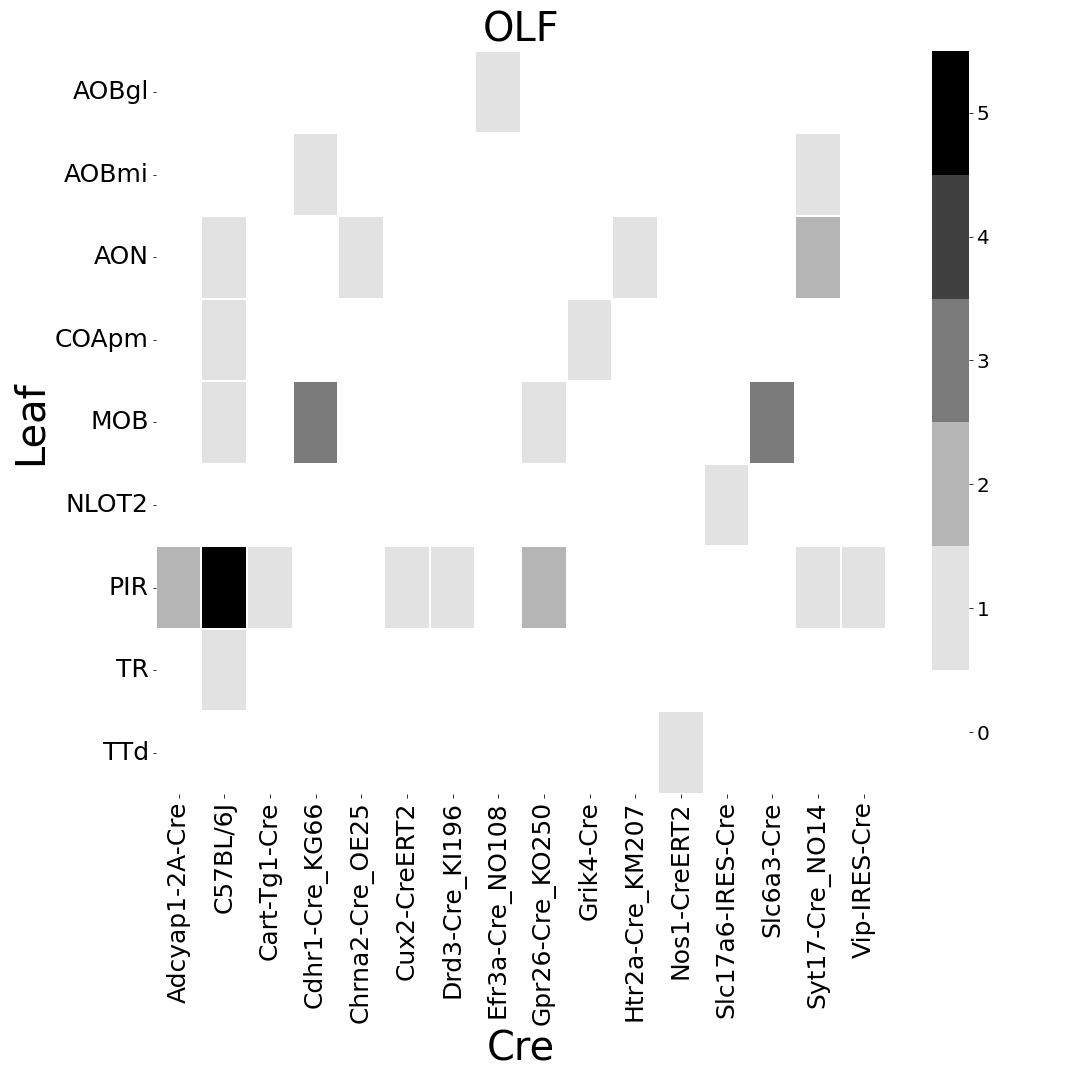
\includegraphics[width = 7in]{figs/OLF centroid density.png} 
    \label{fig:my_label}
\end{figure}
\newpage

\begin{figure}[H]
    \centering
    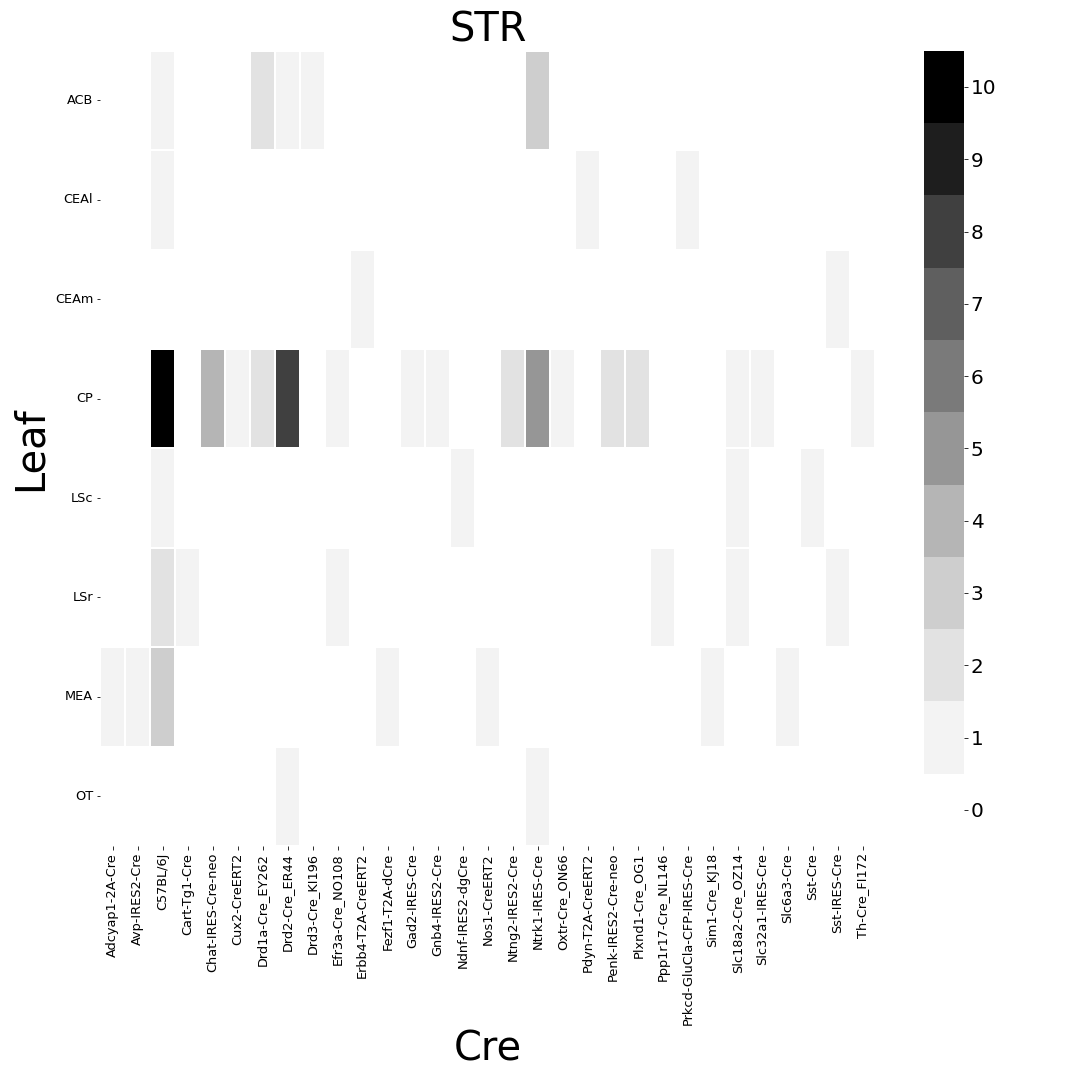
\includegraphics[width = 7in]{figs/STR centroid density.png} 
    \label{fig:my_label}
\end{figure}
\newpage

\begin{figure}[H]
    \centering
    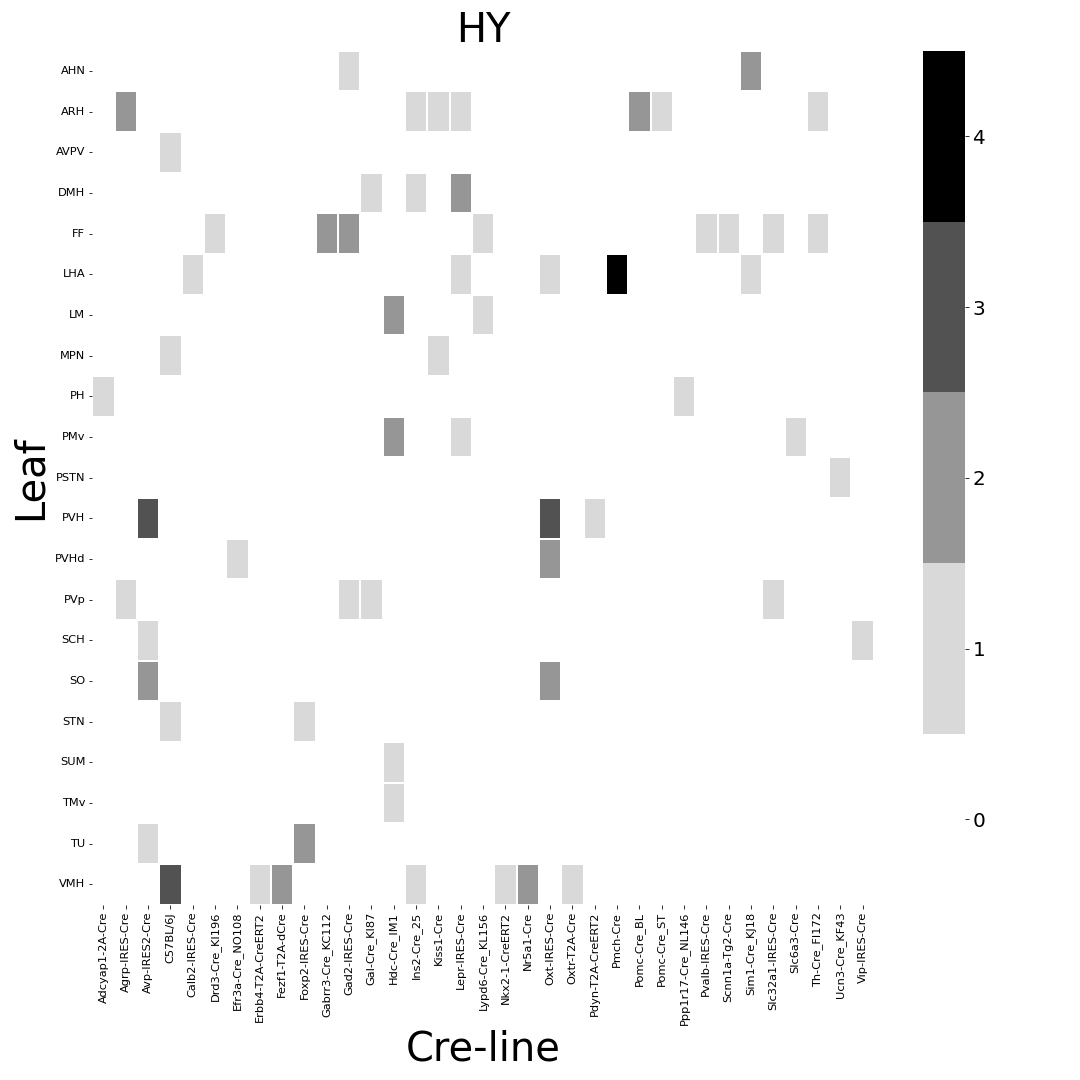
\includegraphics[width = 7in]{figs/HY centroid density.png} 
    \label{fig:my_label}
\end{figure}

\newpage

\subsection{Distances between structures}

\begin{figure}[H]
    \centering
    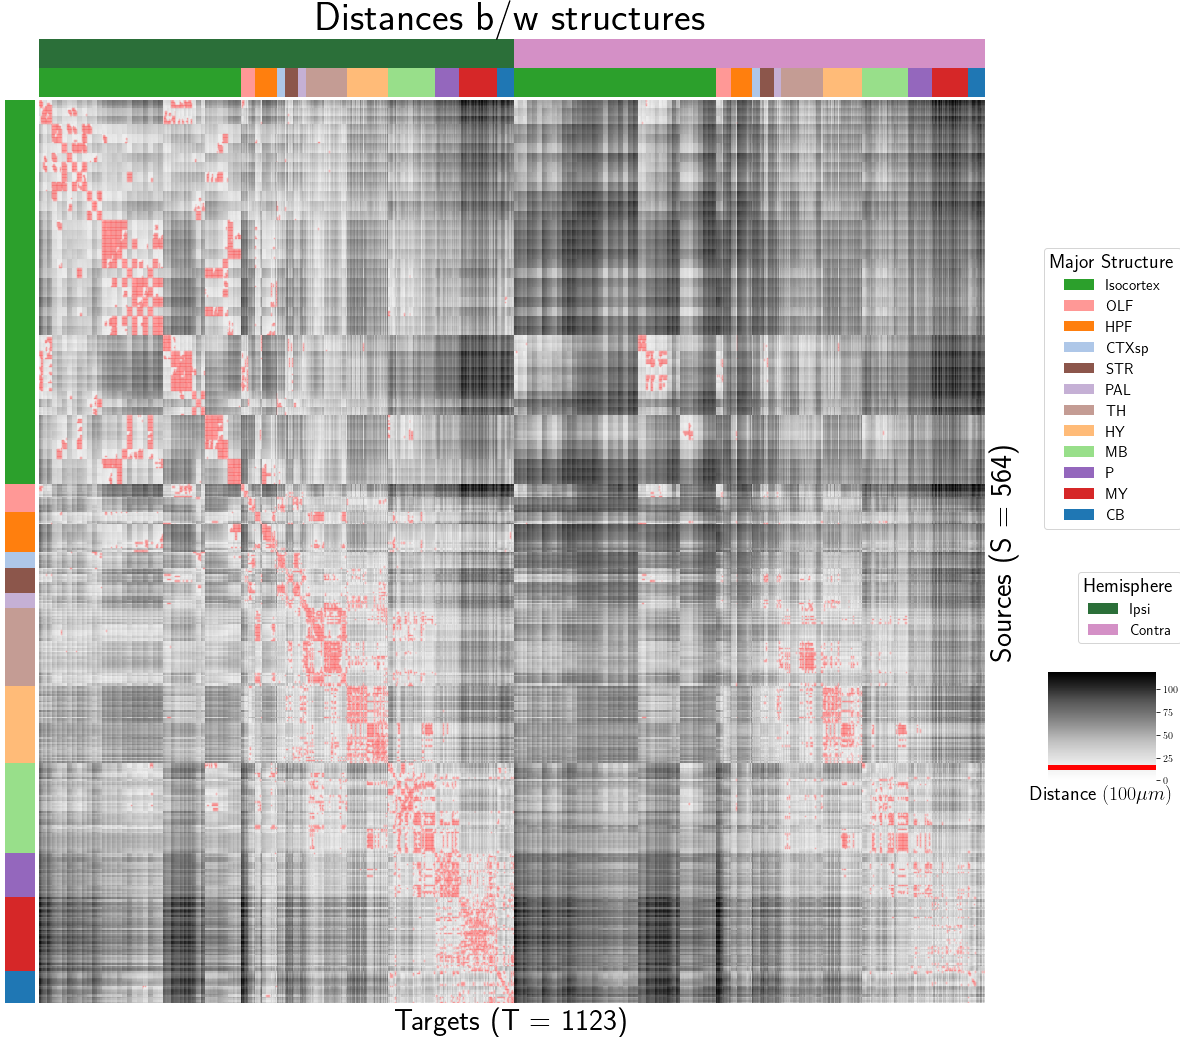
\includegraphics[width = 7in]{analyses/paper/figures/distances_leafs.png} 
    \caption{Distance between structures.  Short-range connections are masked in red}
    \label{fig:dist_bw_str}
\end{figure}

\newpage

\subsection{Model evaluation}
\label{supp_sec:model-evaluation}

We give information on the quality of our models.
This includes the sizes of our evaluation sets in leave-one-out cross-validation and additional losses in the injection-normalized case.


\paragraph{Number of experiments in evaluation sets}

In order to compare between methods, we therefore restrict to the smallest set of evaluation indices, which is to say, virus-leaf combinations that are present at least twice. 
This means that our evaluation set in size is smaller than our evaluation set is smaller in size than our overall list of experiments.


\begin{table}[H]
\small
\begin{tabular}{lrrr}
\toprule
{} &  Total &  Cre-Leaf & Cre-leaf over threshold \\
\midrule
Isocortex &     36 &         4  & 4\\
OLF       &      7 &         2 & 2\\
HPF       &    122 &        62 & 59\\
CTXsp     &     85 &        41 & 38\\
STR       &   1128 &       732& 7 \\
PAL       &     68 &        18 & 17\\
TH        &     46 &         7& 7 \\
HY        &     35 &        17& 17 \\
MB        &     33 &         8 & 8\\
P         &     30 &        11& 11\\
MY        &     78 &        45 & 44\\
CB        &     83 &        29& 29 \\
\bottomrule
\end{tabular}
\caption{Number of experiments available to evaluate models in leave-one-out cross validation. 
Models that rely on a finer granularity of modeling have less data available to validate with.} 
\label{tab:eval_size}
\end{table}

\newpage

\paragraph{Injection-normalized losses}
To compare with the injection-normalization procedure from \citet{Knox2019-ot}, we also remove experiments with small injection, and here give results for this slightly reduced set using injection-normalization.
That is, instead of dividing the projection signal of each experiment by its $l1$ norm, we divide by the $l1$ norm of the corresponding injection signal.
We find that setting a summed injection-signal of threshold of $1$ is sufficient for evading pathological edge cases in this normalization, while still retaining a large evaluation set.

\begin{table}[H]
\begin{tabular}{lrrrrrrr}
\toprule
$\widehat f$ &           Mean & \multicolumn{5}{l}{NW} &     EL \\
$\mathcal D$ & $I_c \cap I_L$ & $I_c \cap I_M$ & $I_c \cap I_L$ &  $I_L$ & $I_{wt} \cap I_M$ &  $I_M$ &  $I_L$ \\
\midrule
Isocortex &          0.413 &          0.453 &          0.408 &  0.538 &             0.528 &  0.528 &  \textbf{0.396} \\
OLF       &          0.499 &          0.504 &          0.494 &  0.441 &             0.543 &  0.543 &  \textbf{0.437} \\
HPF       &          0.336 &          0.483 &          0.332 &  0.444 &             0.501 &  0.501 & \textbf{ 0.321} \\
CTXsp     &          0.497 &          0.497 &          0.497 &  0.497 &             0.497 &  0.497 &  0.497 \\
STR       &          0.359 &          0.386 &          0.359 &  0.364 &             0.433 &  0.433 &\textbf{  0.322} \\
PAL       &          0.519 &          0.497 &          0.519 &  0.436 &             0.459 &  0.459 &\textbf{  0.434} \\
TH        &          0.769 &          0.767 &          0.769 &  \textbf{0.514} &             0.539 &  0.539 &  0.556 \\
HY        &          0.414 &          0.439 &          0.414 &  0.441 &             0.452 &  0.452 & \textbf{ 0.399} \\
MB        &          0.459 &          0.396 &          0.397 &  0.358 &         \textbf{    0.324 }& \textbf{ 0.324 }&  0.403 \\
P         &          \textbf{0.562 }&    \textbf{     0.562 }&      \textbf{    0.562 }&  0.758 &             0.764 &  0.764 &  \textbf{0.562} \\
MY        &          0.699 &          0.552 &          0.621 &  \textbf{0.439 }&             0.578 &  0.578 & \textbf{ 0.439} \\
CB        &          0.849 &          0.689 &          0.849 &  0.500 &             0.615 &  0.615 & \textbf{ 0.495} \\
\bottomrule
\end{tabular}
\caption{Losses from leave-one-out cross-validation of candidate for injection-normalized structural connectivity on injection-thresholded evaluation set. \textbf{Bold} numbers are best for their major structure.} 
\label{tab:eval_size}
\end{table}

\newpage
\paragraph{Projection-normalized losses on thresholded set}

We also give results for the projection-normalization procedure from the main text on this reduced subset.

\begin{table}[H]
\begin{tabular}{lrrrrrrr}
\toprule
$\widehat f$ &           Mean & \multicolumn{5}{l}{NW} &     EL \\
$\mathcal D$ & $I_c \cap I_L$ & $I_c \cap I_M$ & $I_c \cap I_L$ &  $I_L$ & $I_{wt} \cap I_M$ &  $I_M$ &  $I_L$ \\
\midrule
Isocortex &          0.229 &          0.248 &          0.224 &  0.274 &             0.269 &  0.269 &  \textbf{0.217} \\
OLF       &          0.193 &          0.233 &          0.191 &   \textbf{0.135} &             0.179 &  0.179 &  0.138 \\
HPF       &          0.178 &          0.342 &          \textbf{ 0.172 }&  0.212 &             0.235 &  0.235 &   \textbf{0.172} \\
CTXsp     &          \textbf{ 0.621 }&      \textbf{     0.621 }&       \textbf{    0.621} &   \textbf{0.621 }&            \textbf{  0.621} &   \textbf{0.621 }&   \textbf{0.621 }\\
STR       &          0.128 &         \textbf{  0.117} &          0.124 &  0.171 &             0.234 &  0.234 &  0.125 \\
PAL       &          0.203 &          0.205 &          0.203 &  0.295 &             0.291 &  0.291 & \textbf{  0.188 }\\
TH        &          0.673 &          0.664 &          0.673 &   \textbf{0.358} &             0.379 &  0.379 &  0.417 \\
HY        &          0.358 &          0.378 &          0.351 &  0.331 &             0.312 &   \textbf{0.312} &  0.314 \\
MB        &          0.168 &          0.191 &         \textbf{ 0.160 }&  0.199 &             0.202 &  0.202 & \textbf{ 0.160} \\
P         &          0.292 &          0.292 &          0.292 &  0.299 &             0.299 &  0.299 &\textbf{  0.287 }\\
MY        &          0.268 &          0.347 &          0.268 &  \textbf{0.167} &             0.189 &  0.189 &  0.196 \\
CB        &          0.062 &          0.062 &          0.062 &  0.068 &             0.108 &  0.108 &  \textbf{0.061 }\\
\bottomrule
\end{tabular}
\caption{Losses from leave-one-out cross-validation of candidate for normalized structural connectivity on injection-thresholded evaluation set. \textbf{Bold} numbers are best for their major structure.}
\label{tab:crossvalidation}
\end{table}



\newpage 
\section{Supplemental methods}
\label{supp_sec:methods}

This section consists of additional information on preprocessing of the neural connectivity data, estimation of connectivity, and matrix factorization.

\subsection{Data preprocessing}
\label{supp_sec:dp}

Several data prepreprocessing steps take place prior to evaluations of the connectivity matrices.
These steps are described in Algorithm \pre.
The arguments of this normalization process - injection signals $x(i)$, projection signals $y(i)$, injection fraction $F(i)$, and data quality mask $q(i)$ - were downloaded using the Allen SDK. %and injection fraction $F(i)$ 
The injections and projection signals $ \mathcal B \to \mathbb [0,1]$ were segmented manually in histological analysis.
The projection signal gives the proportion of pixels within the voxel displaying fluorescence, and the injection signal gives the proportion of pixels within the histologically-selected injection subset displaying fluorescence.
The injection fraction $ \mathcal B \to \mathbb [0,1]$ gives the proportion of pixels within each voxel in the injection subset.
Finally, the data quality mask $ \mathcal B \to \mathbb \{0,1\}$ gives the voxels that have valid data.

%We also have a map $A: \mathbb R \to \mathbb R^{|S|}$ where $S$ is the number of structures that takes the average value for voxels in that structure
Our preprocessing makes use of the above ingredients, as well as several other essential steps.
First, we compute the weighted injection centroid
\begin{eqnarray*}
c(i) &= \sum_{l \in \mathcal B} x(i)(l) l
\end{eqnarray*}
where $x(i)(l)$ is the injection density at location $l \in \mathbb R^3$.
Given a regionalization $\mathcal R$ from the Allen SDK, we can also access regionalization map $R: \mathcal B  \to \mathcal R $.
This induces a functional of connectivities from the space of maps $\{\mathcal X = x: \mathcal B \to [0,1]$
\begin{eqnarray*}
1_{\mathcal R}: \mathcal X &\to \mathcal R \times \mathbb R_{\geq 0} \\
x &\mapsto \sum_{l \in r}  x(l)  \text{ for } r \in \mathcal R.
\end{eqnarray*}
%This map depends on the choice of regionalization; we regionalize at the leaf level.
We also can restrict a signal to a individual structure as
\begin{eqnarray*}
1 |_s :  \mathcal X &\to  \mathcal X \\
 x(l) &= \begin{cases} 
 x(l) \text{ if } l \in S \\
 0 \text{ otherwise }.
 \end{cases}
\end{eqnarray*}
Finally, given a vector or array $a \in \mathbb R^T$, we have the $L1$ normalization map
\begin{eqnarray*}
n: a &\mapsto \frac{a}{\sum_{j = 1}^T a_j}.
\end{eqnarray*}

We define these objects as functions and functionals, but this is for notational convenience and non-essential.
A function $x(i):\mathcal B \to [0,1]$ is mathematically equivalent to the graph $\mathcal G(x(i)) \in \mathcal B \times [0,1]$.
As an abuse of notation, we define $x \odot x' := z$ such that $z(l) = x(l) x'(l)$ for all $l \in \mathcal B$.
Also, denote $m(i)$ as the major structure containing experiment $i$.
We then can write the preprocessing algorithm.

\begin{algorithm}[H]
\floatname{algorithm}{\pre}%{\preprocess}
\caption{{\bf Input} Injection $x(i)$, Projection $y(i)$, Injection centroid $c(i) \in \mathbb R^3$, injection fraction $F(i)$, data quality mask $q(i)$}
\label{alg:preprocess}
\begin{algorithmic}
\State Injection fraction $x_F(i) \gets x(i) \odot F(i)$
\State Data-quality censor $y_q (i) \gets  \odot y(i) \odot q(i) , x_q(i) \gets x_F(i) \odot q(i)$
\State Restrict injection $x_m(i) = 1 |_{m(i)} x_q(i) $.
\State Compute centroid $c(i)$ from $x_m(i) $
\State Regionalize $\tilde y_{\mathcal T} (i) \gets 1_{\mathcal T}(  y_q(i))$
\State Normalize $ y_{\mathcal T} (i) \gets n(\tilde y_{\mathcal T} (i) )$
 \State {\bf Output}$\tilde y_{\mathcal T} (i) $, $c(i)$ 
\end{algorithmic}
\end{algorithm}


%The data-quality censor is established by \skcomment{fill}
%We find the $l2$ norm not appropriate in a few ways 1) there is not a clear inner product structure on the connectome.
%doesn't matter if we normalize prior to regionalization as long as we don't correct for density of the target region.
%which, due to normalization, can be rewritten as simply the $l2$ loss $\|y - \hat y\|.$  Note that, due to normalization, $\|y - \hat y\| = \langle y - \hat y , y - \hat y \rangle = 2 - 2 \langle y, \hat y\rangle $, and, applying normalization again, $ \langle y, \hat y\rangle $ is the vector cosine of $\hat y$ and $y$.

\newpage
\subsection{Estimators}
\label{supp_sec:estimators}
As mentioned previously, we can consider our estimators as modeling a connectivity vector $f_{\mathcal T} (v,s)  \in \mathbb R_{\geq 0}^T$.
Thus, for the remainder of this section, we will discuss only $f (v,s)$.
We review the Nadaraya-Watson estimator from  \citet{Knox2019-ot}, and describe its conversion into our cell-class specific Expected Loss estimator.

\subsubsection{Centroid-based Nadaraya-Watson}

In the Nadaraya-Watson approach of \citet{Knox2019-ot}, the injection is considered only through its centroid $c(i)$, and the projection is considered regionalized.
%The prediction for a given region is then given by the integral of predictions over that region, which is computed as a sum over voxels.
That is,
\begin{eqnarray*}
f_*(i) = \{c(i), y_{\mathcal T}(i)\}.
\end{eqnarray*}
Since the injection is considered only by its centroid, this model only generates predictions for particular locations $l$, and the prediction for a structure $s$ is given by integrating over locations within the structure
\begin{eqnarray*}
\label{eq:regionalize}
f^* (\hat f (f_*(\mathcal D))) (v,s) = \sum_{l \in s} \hat f (f_*(\mathcal D(I))) (v,l ).
\end{eqnarray*}
Here, $I$ is the training data, and $\hat f$ is the Nadaraya-Watson estimator
\begin{eqnarray*}
\hat f_{NW}( c(I) , y_{\mathcal T}(I) ) (l) :=  \sum_{i \in I} \frac{ \omega_{i l}}{\sum_{i \in I} \omega_{i l}} y_{\mathcal T}(i)
\end{eqnarray*}
where $\omega_{i l } := \exp( - \gamma d( l , c(i))^2 )$ and $d$ is the Euclidean distance between centroid $c(i)$ and voxel with position $l$.

Several facets of the estimator are visible here. %$f_{NW}^{\gamma}$ is the Nadaraya-Watson estimator with smoothing given by inverse-bandwidth $\gamma$.
A smaller $\gamma$ corresponds to a greater amount of smoothing, and the index set $I \subseteq  \{1:n\}$ generally depends on $s$ and $v$.
Fitting $\gamma$ via empirical risk minimization therefore bridges between $1$-nearest neighbor prediction and averaging of all experiments in $I$.
In \citet{Knox2019-ot}, $I$ consisted of experiments sharing the same brain division, i.e. $I = I_m$, while restricting of index set to only include experiments with the same cell class gives the class-specific Cre-NW model.
Despite this restriction, we fit $\gamma$ for each $m$ rather than a smaller subset like $s$ or $v$.
That is,
\begin{eqnarray}
\label{eq:gamma_sel}
\widehat \gamma_m =  \arg \min_{\gamma \in \mathbb R_{\geq 0}} \frac{1}{|\{s,v\}|} \sum_{s,v \in \{m,\mathcal V\}} \frac{1}{ |I_{s} \cap I_v |} \sum_{i \in (I_{s} \cap I_v ) } \ell (y_{\mathcal T}(i)), \hat f_{\mathcal T} (f_*(\mathcal D(v,s) \setminus i)) .
\end{eqnarray}

\newpage
\subsubsection{The Expected-Loss estimator}

\label{supp_sec:el}

Besides the injection location, the targeted cell class also influences projection.
Since Cre-lines that target similar classes are induce similar projections, and including similar Cre-lines in the Nadaraya-Watson estimator increases effective sample size, we introduce an estimator that assigns a predictive weight to each training point that depends both on its centroid-distance and Cre-line.
This weight is determined by the expected prediction error of each of the two feature types, as determined by cross-validation.
For this reason, we call this the Expected Loss Estimator.
The resulting weights are then utilized in a Nadaraya-Watson estimator in a final prediction step.
%It shares thefine-scale spatial resolution with \citet{Knox2019-ot}, but in addition enables us to model a particular cell-class $v$.

We formalize Cre-line behavior as the average regionalized projection of a Cre-line in a given structure (i.e. leaf).
This vectorization of categorical information is known as \textbf{target encoding}, and we define this as $\bar y_{\mathcal T,s,v} := \frac{1}{|I_s \cap I_v|}  \sum_{i \in (I_s \cap I_v)} y_{\mathcal T}(i)$.
We define a \textbf{Cre-distance} in a leaf to be the distance between the target-encoded projections of two Cre-lines.
The relative predictive accuracy of Cre-distance and centroid distance is determined by fitting a surface of projection distance as a function of Cre-distance and centroid distance. 

In mathematical terms, our full feature set consists of the centroid coordinates and the target-encoded means of the combinations of virus type and injection-centroid structure.
That is, 
\begin{eqnarray*}
f_*({\mathcal D}_i) = \{c(i) , \{\bar y_{\mathcal T,s,v}  \forall v \}, y_{\mathcal T}(i) \}.
\end{eqnarray*}
$f^*$ is defined as in \eqref{eq:regionalize}.
The expected loss estimator is then 
\begin{eqnarray*}
\hat f_{EL} ( c(I),y_{\mathcal T} (I))(l,v) :=  \sum_{i \in I} \frac{ \nu_{ilv} }{\sum_{i \in I}  \nu_{ilv}  } y_{\mathcal T}(i)
\end{eqnarray*}
where
\begin{eqnarray*}
\nu_{ilv} := \exp (- \gamma g( d(l, c(i))^2, d(\bar y_{\mathcal T,s,v} , \bar y_{\mathcal T,s,v(i)}  )^2))
\end{eqnarray*}
and $s$ is the structure containing $l$.

The key step therefore is finding a suitable $g$ with which to weight the positional and Cre information.
Note that $g$ must be a concave, non-decreasing function of its arguments with with $g(0,0) = 0$, then $g$ defines a metric on the product of the metric spaces defined by experiment centroid and target-encoded cre-line, and $\hat f_{EL}$ is a Nadaraya-Watson estimator. 
A derivation of this fact is given later in this section, and we therefore use shape-constrained B-splines to estimate $g$.
Similarly to the Nadaraya-Watson model, we make the decision to fit a $g$ separately for each major brain division.
We can then select $\hat \gamma$ as in \ref{eq:gamma_sel}.

\newpage

\begin{figure}[H]
\begin{tabular}[t]{cc}
\subfloat[]{
    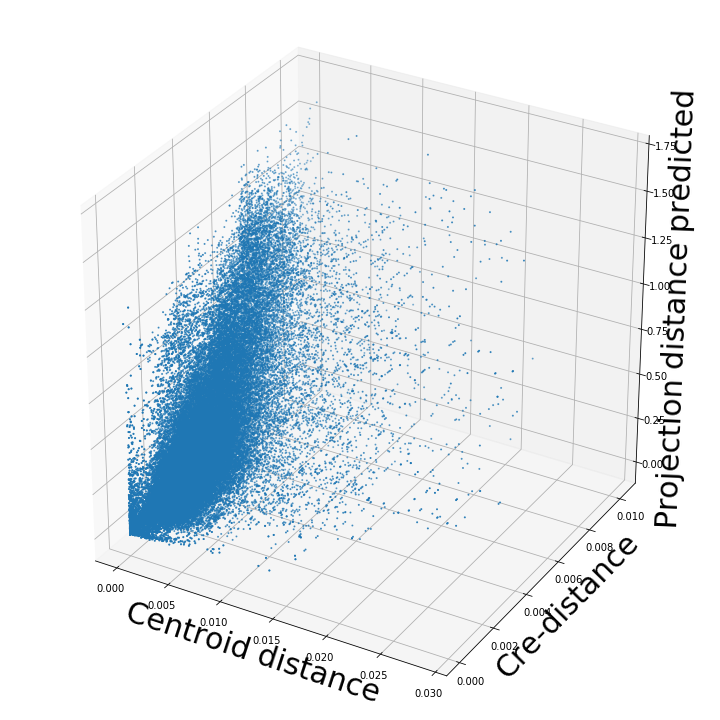
\includegraphics[width = 2.1in]{figs/figsforpres/315_summary_scatter.png}
   % \caption{Isocortex loss distribution}
    \label{fig:expected_loss} 
   }
    &
    \subfloat[]{
    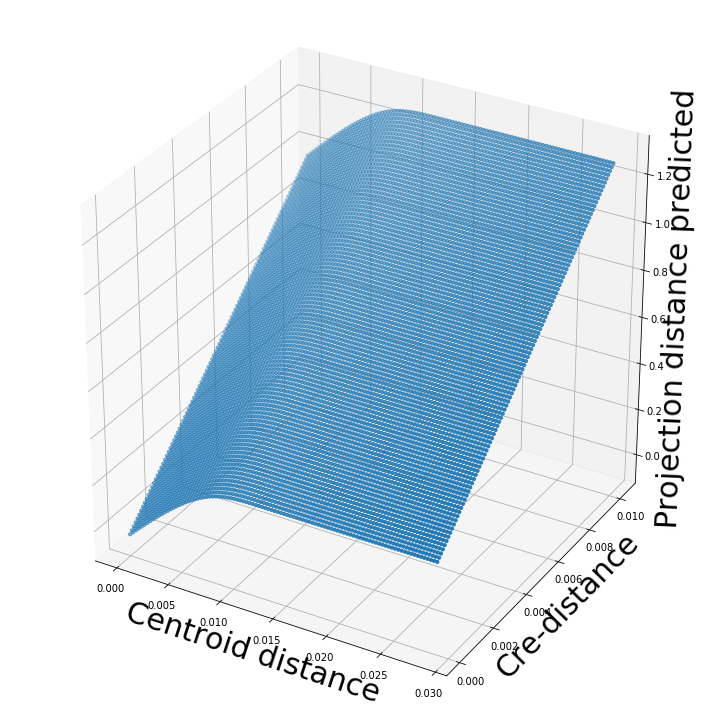
\includegraphics[width = 2.1in]{figs/figsforpres/315_summary_surface.png}
   % \caption{$\hat g$ fit to expected-loss using shape-constrained splines}
   \label{fig:expected_loss_surface}
    }
   \end{tabular}
   \caption{Fitting $g$.
   \ref{fig:expected_loss} Distribution of projection errors against centroid distance and cre-distance in Isocortex.
    \ref{fig:expected_loss_surface} $\hat g$ found using B-splines.
    }
   \end{figure}
   
  \newpage
  
%This contrasts with the models in \citet{Knox2019-ot} and \citet{Oh2014-kh}, where connectivity was directly estimated by $\hat f$ a function of $S$ without an integral.
%Since we wish to weight similar points more highly, we weight distances in cre-space and centroid-space by how well they predict the response variable.
%Due to the fact that the cre-space is defined with respect to the response variable, points are removed from their cre-mean prior to cross-validation.
%Figure shows an example of such an estimated $g$.

%In the low-sample size setting, it is worth utilizing points from similar groups.

%\newpage

%\begin{algorithmic}
%\label{alg:model}
%\begin{algorithm}{Injection centroids $c(1:n)$, normalized projections $n(r(y(1:n)))$, viruses $v(1:n)$. target centroid $c$, target virus $v$}
%\STATE Get structures $s(1:n) = r(c(1:n))$, $s = r(c)$
%\STATE Target encode $v(1:n)$ and $v$ with $n(r(y(1:n)))$
%\STATE Estimate expected loss $l_{ii'} = \hat f (\|c(i) - c(i')\|_2^2, \|t(v(i)) - t(v(i'))\|_2^2)$
% \RETURN $\tilde y(i)$ (optional $\tilde x(i)$ )
%\end{algorithm}
%\end{algorithmic}


\newpage
%\subsubsection{The expected-loss estimator}
\paragraph{Justification of shape constraint}

The shape-constrained expected-loss estimator introduced in this paper is, to our knowledge, novel.
It should be considered an alternative method to the classic weighted kernel method.
While we do not attempt a detailed theoretical study of this estimator, we do establish the need for the shape constraint in our spline estimator.
Though this fact is probably well known, we prove a (slightly stronger) version here for completeness.

\begin{proposition}
Given a collection of metric spaces $X_1, ... X_n$ with metrics $d_1 ... d_n$ (e.g. $d_{centroid}, d_cre$), and a function $f: (X_1 \times X_1) ... \times (X_n  \times X_n) = g(d_1(X_1 \times X_1),... d_n(X_n \times X_n))$, then then $f$ is a metric iff $g$ is concave, non-decreasing and $g(d) = 0 \Longleftrightarrow d = 0$.
\end{proposition}

\begin{proof}
We first show $g$ satisfying the above properties implies that $f$ is a metric.
\begin{itemize}
    \item The first property of a metric is that $f(x,x') = 0 \Longleftrightarrow x = x'$.  The left implication: $x = x' \implies f(x_1, x_1', ... x_n, x_n') = g(0,....,0)$, since $d$ are metrics.  Then, since $g(0) = 0$, we have that $f(x,x') = 0$. The right implication: $f(x,x') = 0 \implies  d = 0 \implies x = x'$ since $d$ are metrics.
    \item The second property of a metric is that $f(x,x') = f(x',x)$. This follows immediately from the symmetry of the $d_i$, i.e. $f(x,x') = f(x_1, x_1', ... x_n, x_n') = g(d_1(x_1, x_1'), ... d_n(x_n, x_n')) = g(d_1(x_1', x_1), ... d_n(x_n', x_n)) =  f(x_1', x_1, ... x_n', x_n) = f(x',x)$.
    \item The third property of a metric is the triangle inequality: $f(x, x') \leq f(x, x^*) +  f(x^*, x') $.  To show this is satisfied for such a $g$, we first note that $f(x,x') = g(d(x,x')) \leq g(d(x, x^*) + d(x^*, x')) $ since g is non-decreasing and by the triangle inequality of $d$. Then, since $g$ is concave, $g(d(x, x^*) + d(x^*, x')) \leq g(d(x, x^*)) + g(d(x^*, x')) = f(x,x^*) + f(x^*, x')$.
    %or $ f(x_1, x_1', ... x_n, x_n') \leq f(x_1, x_1^*, ... x_n, x_n^*) + f(x_1', x_1^*, ... x_n', x_n^*)$.  To show this is satisfied for such a $g$, we first note $f(x_1, x_1', ... x_n, x_n') = g(d_1(x_1, x_1'),... d_n(x_n ,x_n')) \leq g(d_1(x_1, x_1*) + d_1(x_1', x_1*) ,... , d_n(x_n ,x_n*) + d_n(x_n' ,x_n*))$ since g is non-decreasing and by the triangle inequality on d. Then $g(d_1(x_1, x_1*) + d_1(x_1', x_1*) , ... , d_n(x_n , x_n*) + d_n(x_n' ,x_n*)) < f(x_1, x_1*, ... x_n, x_n*) + f(x_1', x_1*, ... x_n', x_n*)$ since $g$ is concave.
    
    %Lemma: h(a+ b) < h(a) + h(b) for a concave increasing function h.  
%Pf: h(a+b) - h(b) < h(a) - h(0) since rate of increase is decreasing.
\end{itemize}

We then show that $f$ being a metric implies that $g$ satisfies the above properties.
\begin{itemize}
    \item The first property is that $g(d) = 0 \Longleftrightarrow d = 0$. We first show the right implication: $g(d) = 0$, and $g(d) = f(x,x')$, so $x = x'$ (since $f$ is a metric), so $d = 0$. We then show the left implication: $d = 0 \implies x = x'$, since $d$ is a metric, so $f(x,x') = 0,$ since $f$ is a metric, and thus $g(d) = 0$.
    %\item 
    %$f$ is a metric, so $f(x,x') = 0 \Longleftrightarrow x = x'$.  Then, since $f(x,x') = g(d (x,x') )$ which $\implies g(0,\dotsc 0) = 0$ since $g$ is increasing.
    \item The second property is that $g$ is non-decreasing. We proceed by contradiction.
    Suppose g is decreasing in argument $d_1$ in some region $[l, u]$ with $0 < l< u$.
    Then $g(d_1(0, l), 0) \geq g(d_1(0, 0), 0) + g(d_1(0, u), 0) = g(d_1(0, u),0)$, which violates the triangle inequality on f. Thus, decreasing $g$ means that $f$ is not a metric, so $f$ a metric implies non-decreasing $g$.
    \item The final property is that $g$ is concave. We proceed by contradiction. Suppose $g$ is strictly convex. Then there exist vectors $d, d'$ such that $g(d + d')  < g(d) + g(d')$.  Assume that $d$ and $d'$ only are non-zero in the first position, and $d = d(0, x), d' = d(0,x')$.  Then, $f(0,x) + f(0,x') <  f(0,x+ x')$, which violates the triangle inequality on $f$.  Therefore, $g$ must be concave.
\end{itemize}

\end{proof}

\newpage

\subsection{Establishing a lower detection limit}
\label{supp_sec:methods_lower}

The lower detection limit of our approach is a complicated consequence of our experimental and analytical protocols.
For example, the Nadaraya-Watson estimator is likely to generate many small false positive connections, since the projection of even a single experiment within the source region to a target will cause a non-zero connectivity in the Nadaraya-Watson weighted average.
On the other hand, the complexities of the experimental protocol itself and the image analysis and alignment can also cause spurious signals.
Therefore, it is of interest to establish a lower-detection threshold below which we have very little power-to-predict, and set estimated connectivities below this threshold to zero.
This should make our estimated connectivities more accurate, especially in the biologically-important sense of sparsity.

We establish this limit with respect to the sum of Type 1 and Type 2 errors
\begin{eqnarray*}
\iota = \sum_{i \in \mathcal E} 1_{y_{\mathcal T}(i) = 0}^T 1_{\hat f_{\mathcal T}(v(i),c(i)) > \tau} + 1_{y_{\mathcal T}(i) > 0}^T 1_{\hat f_{\mathcal T}(v(i),c(i)) < \tau}  .
\end{eqnarray*}

We then select the $\tau$ that minimizes $\iota$.
Results for this approach are given in Supplemental Section \ref{supp:exp_lower}.

\newpage

\subsection{Decomposing the connectivity matrix}
\label{supp_sec:matrix_factor_methods}

We utilize non-negative matrix factorization (NMF) to analyze the principal signals in our connectivity matrix.
Here, we review this approach as applied to decomposition of the distal elements of the estimated connectivity matrix $\widehat {\mathcal C}$ to identify $q$ connectivity archetypes.
Aside from the NMF program itself, the key elements are selection of the number of archetypes $q$ and stabilization of the tendency of NMF to give random results over different initializations. 

\subsubsection{Non-negative matrix factorization}

As discussed in \citet{Knox2019-ot}, one of the most basic processes underlying the observed connectivity is the tendency of each source region to predominantly project to proximal regions.
For example, the heatmap in Supplemental Figure \ref{fig:dist_bw_str} shows intrastructure distances clearly contains a diagonal pattern resembling  the connectivity matrix in \ref{fig:connectome}.
These connections are biologically meaningful, but also unsurprising, and their relative strength biases learned latent coordinate representations away from long-range structures.
For this reason, we establish a $1500 \mu m$ 'distal' threshold within which to exclude connections for our analysis.

%More generally, %This relationship is plotted in \ref{fig:nmf} b), showing that there exists substantial variability that would be impossible to model with low-error in a univariate model, even using the diffusion model suggested in \citet{Knox2019-ot}.
%Second, the specific cell-types targeted by the various cre-lines themselves generate a reduced-dimension space. Under the assumption that cell-type determines projection pattern, we can investigate which cell-types are present in which of the projecting structures.


Given a matrix $X \in \mathbb R_{\geq 0}^{a \times b}$ and a desired latent space dimension $q$, the non-negative matrix factorization is thus
\begin{eqnarray*}
\nmf (\mathcal C, \lambda, q,1_{M}) = \arg \min_{W \in \mathbb R_{\geq 0}^{S \times q}, H\in \mathbb R_{\geq 0}^{q \times T}} \frac{1}{2}\| 1_{M} \odot \mathcal C - WH\|_2^2  + \lambda  (\|H \|_1 + \|W \|_1) .
\end{eqnarray*}
We note the existence of NMF with alternative norms for certain marginal distributions, but leave utilization of this approach for future work \citep{Brunet2004-gi}.

The mask $1_M \in \{0,1\}^{S \times T}$ serves two purposes.
First, it enables computation of the NMF objective while excluding self and nearby connections.
These connections are both strong and linearly independent, and so would unduly influence the $NMF$ reconstruction error over more biologically interesting or cell-type dependent long-range connections.
Second, it enables cross-validation based selection of the number of retained components.

\subsubsection{Cross-validating NMF}

Cross-validation for NMF is somewhat standard but not entirely well-known, and so we review it here.
In summary, a NMF model is first fit on a reduced data set, and an evaluation set is held out.
After random masking of the evaluation set, the loss of the learned model is then evaluated on the basis of successful reconstruction of the held-out values.
This procedure is performed repeatedly, with replicates of random masks at each tested dimensionality $q$.
This determines the point past which additional hidden units provide no reconstructive value.

The differentiating feature of cross-validation for NMF compared with supervised learning is the randomness of the masking matrix $1_M$.
Cross-validation for supervised learning generally leaves out entire observations, but this is insufficient for our situation.
%where $e(\mathcal C)$ is a map that encodes $\mathcal C$ in a learned representation, and $d$ is the decoding reconstruction map.
This is because, given $W$, our $H$ is the solution of a regularized non-negative least squares optimization problem
\begin{eqnarray}
H := \widehat e_W(1_{M} \odot \mathcal C) = \arg \min_{\beta \in \mathbb R_{\geq 0}^{q \times T}} \|1_{M} \odot \mathcal C - W \beta\|_2^2 + \|\beta\|_1.
\label{eq:nmf_nnls}
\end{eqnarray}
The negative effects of an overfit model can therefore be optimized away from on the evaluation set.

A standard solution is to generate uniformly random masks $1_{M(p)} \in \mathbb R^{S \times T}$ where
\begin{align*}
1_{M(p)} (s,t) \sim \text{Bernoulli(p)}.
\end{align*}
NMF is then performed using the mask $1_{M(p)}$ to get $W$.
The cross-validation error is then
\begin{align*}
\epsilon_q &= \frac{1}{R} \sum_{r = 1}^R (\|1_{M(p)_r^C} \odot X - W (\widehat e_W (1_{M(p)_r^C} \odot X ))\|_2^2 
\end{align*}
where $1_{M(p)_r}^C$ is the binary complement of $1_{M(p)_r}$ and $R$ is a number of replicates.
Theoretically, the optimum number of components is then
\begin{align*}
    \widehat q = \arg \min_q \epsilon_q.
\end{align*}
%However, the low decrease in error at higher values of $q$ will motivate us to empirically select a slightly smaller number of components.

\subsubsection{Stabilizing NMF}

The NMF program is non-convex, and, empirically, individual replicates will not converge to the same optima.
One solution therefore is to run multiple replicates of the NMF algorithm and cluster the resulting vectors.
This approach raises the questions of how many clusters to use, and how to deal with stochasticity in the clustering algorithm itself.
We address this issue through the notion of clustering stability \citep{Von_Luxburg2010-lu}.

The clustering stability approach is to generate $L$ replicas of k-cluster partitions $\{C_{kl} : l \in 1 \dots L\}$ and then compute the average dissimilarity between clusterings
\begin{align*}
\xi_k &= \frac{2}{L(L - 1)} \sum_{l = 1}^{L} \sum_{l'= 1}^{l}  d(C_{kl}, C_{kl'}).
\end{align*}
Then, the optimum number of clusters is 
\begin{align*}
\hat k &= \arg \min_k \xi_k.
\end{align*}
A review of this approach is found in \citet{Von_Luxburg2010-qe}.
Intuitively, archetype vectors that cluster together frequently over clustering replicates indicate the presence of a stable clustering.
For $d$, we utilize the adjusted Rand Index - a simple dissimilarity measure between clusterings.
Note that we expect to select slightly more than the $q$ components suggested by cross-validation, since archetype vectors which appear in one NMF replicate generally should appear in others.
We then select the $q$ clusters with the most archetype vectors - the most stable NMF results - and take the median of each cluster to create a sparse representative archetype \citet{Wu2016-gg, Kotliar2019-yj}.
We then find the according $H$ using Program \ref{eq:nmf_nnls}.
Experimental results for these cross-validation and stability selection approaches are given in Supplemental Section \ref{supp_sec:matrix_factor_results}.

\newpage

\section{Supplemental Experiments}
\label{supp_sec:exp}

\subsection{Establishing a lower limit of detection}
\label{supp:exp_lower}

We give results on the false detection rate at different limits of detection.
These conclusively show that $10^{-6}$ is the good threshold for our normalized data.
\begin{figure}[H]
    \centering
    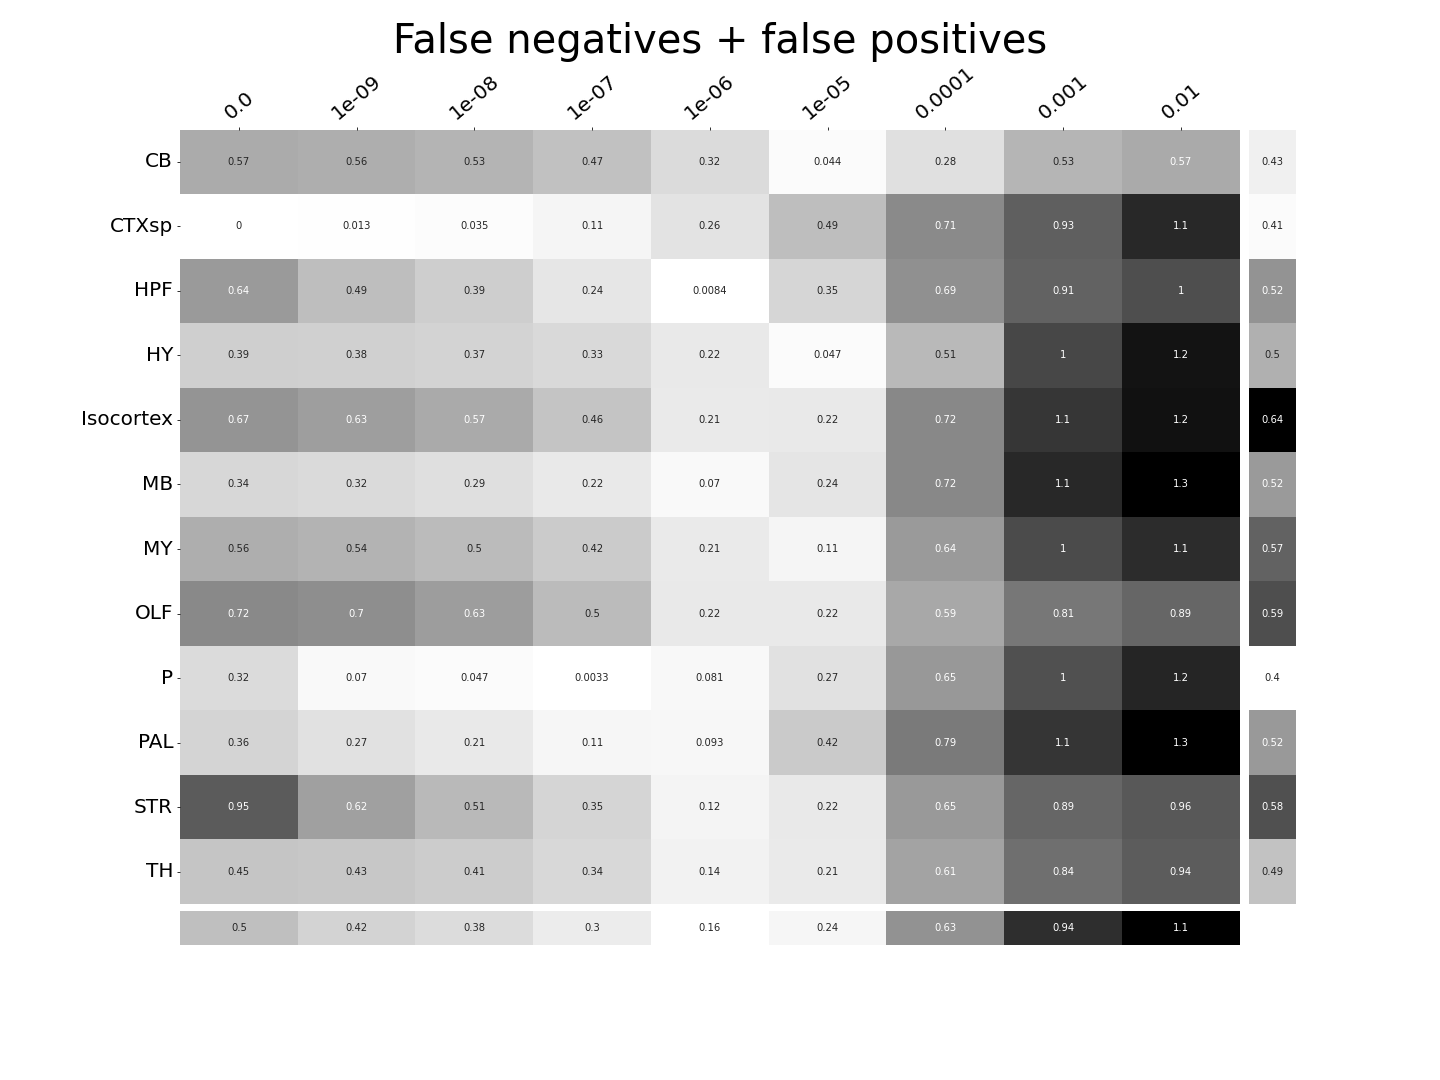
\includegraphics[width = 7in]{paper/Threshold.png}
    \label{fig:threshold}
    \caption{$\tau$ at different limits of detection in different major structures.  $10^{-6}$ is clearly the optimal detection threshold.}
\end{figure}

\newpage

\subsection{Loss subsets}
\label{supp_sec:loss_subsets}

We report model accuracies for our $EL$ model by neuron class and structure.
These expand upon the results in Table \ref{tab:crossvalidation} and give more specific information about the quality of our estimates. 

\begin{figure}[H]
    \centering
    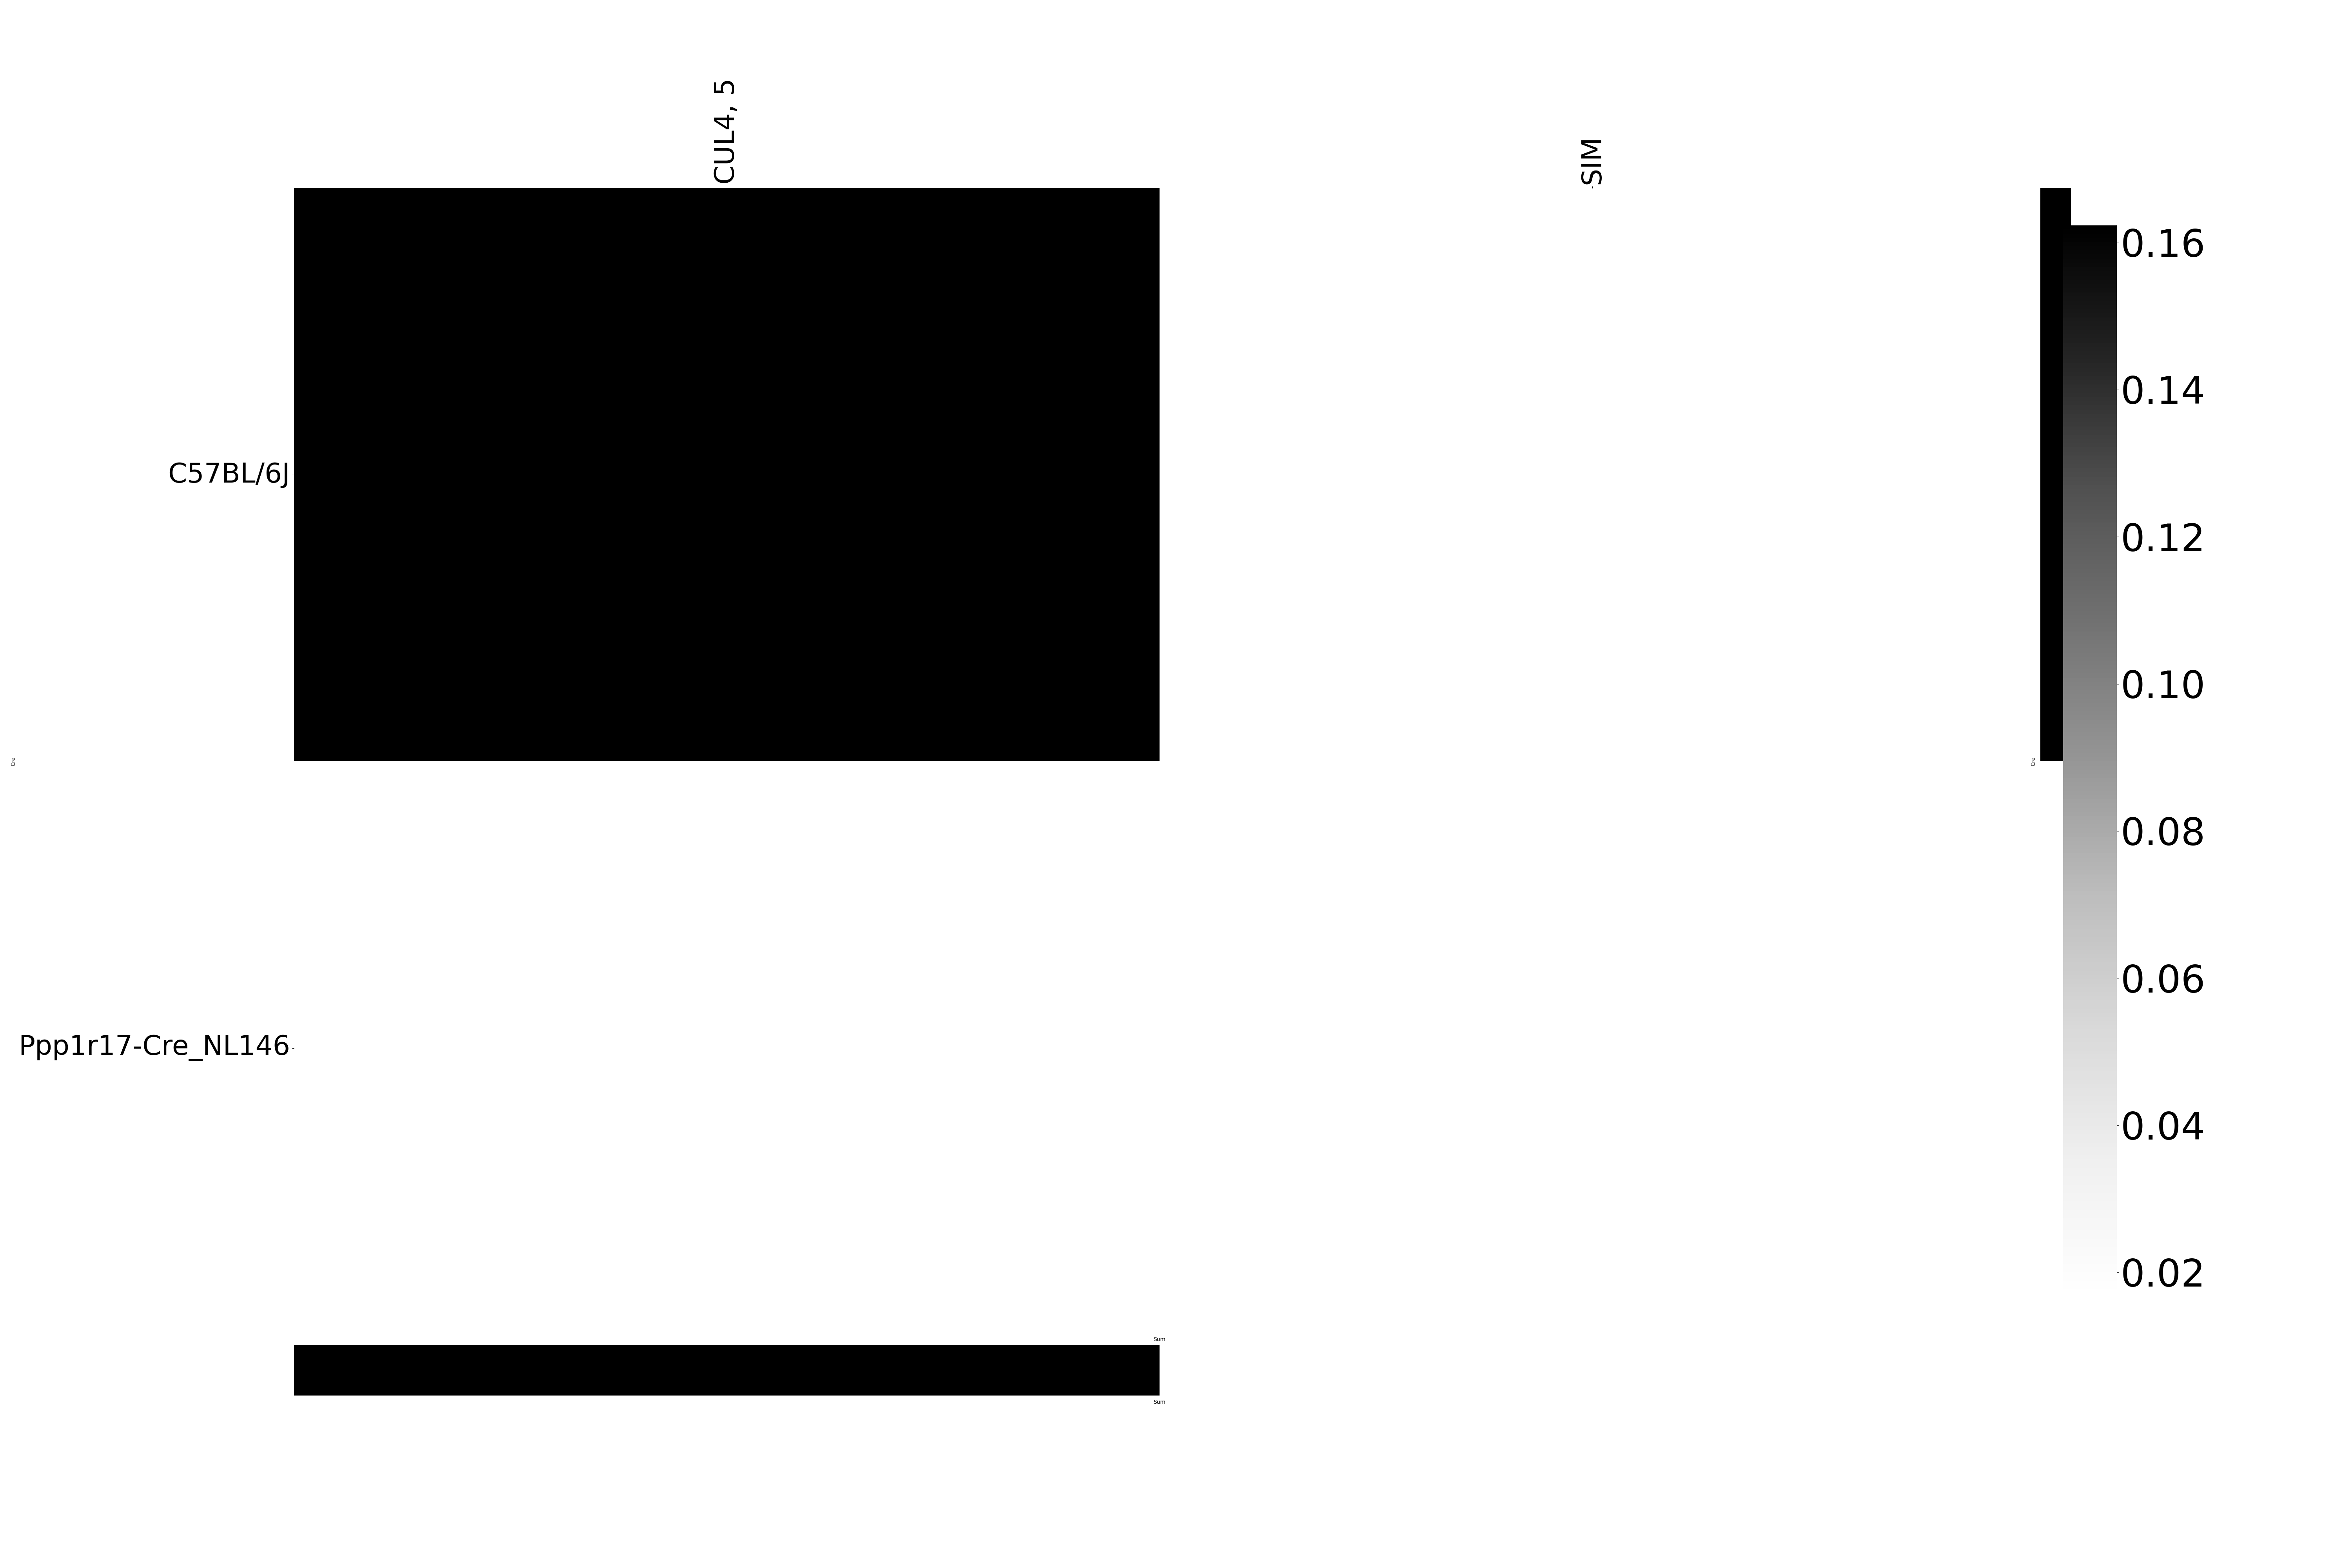
\includegraphics[width = 7in]{figs/lossdetails_512.png} 
    \label{fig:distances}
    \caption{}
\end{figure}

\begin{figure}[H]
    \centering
    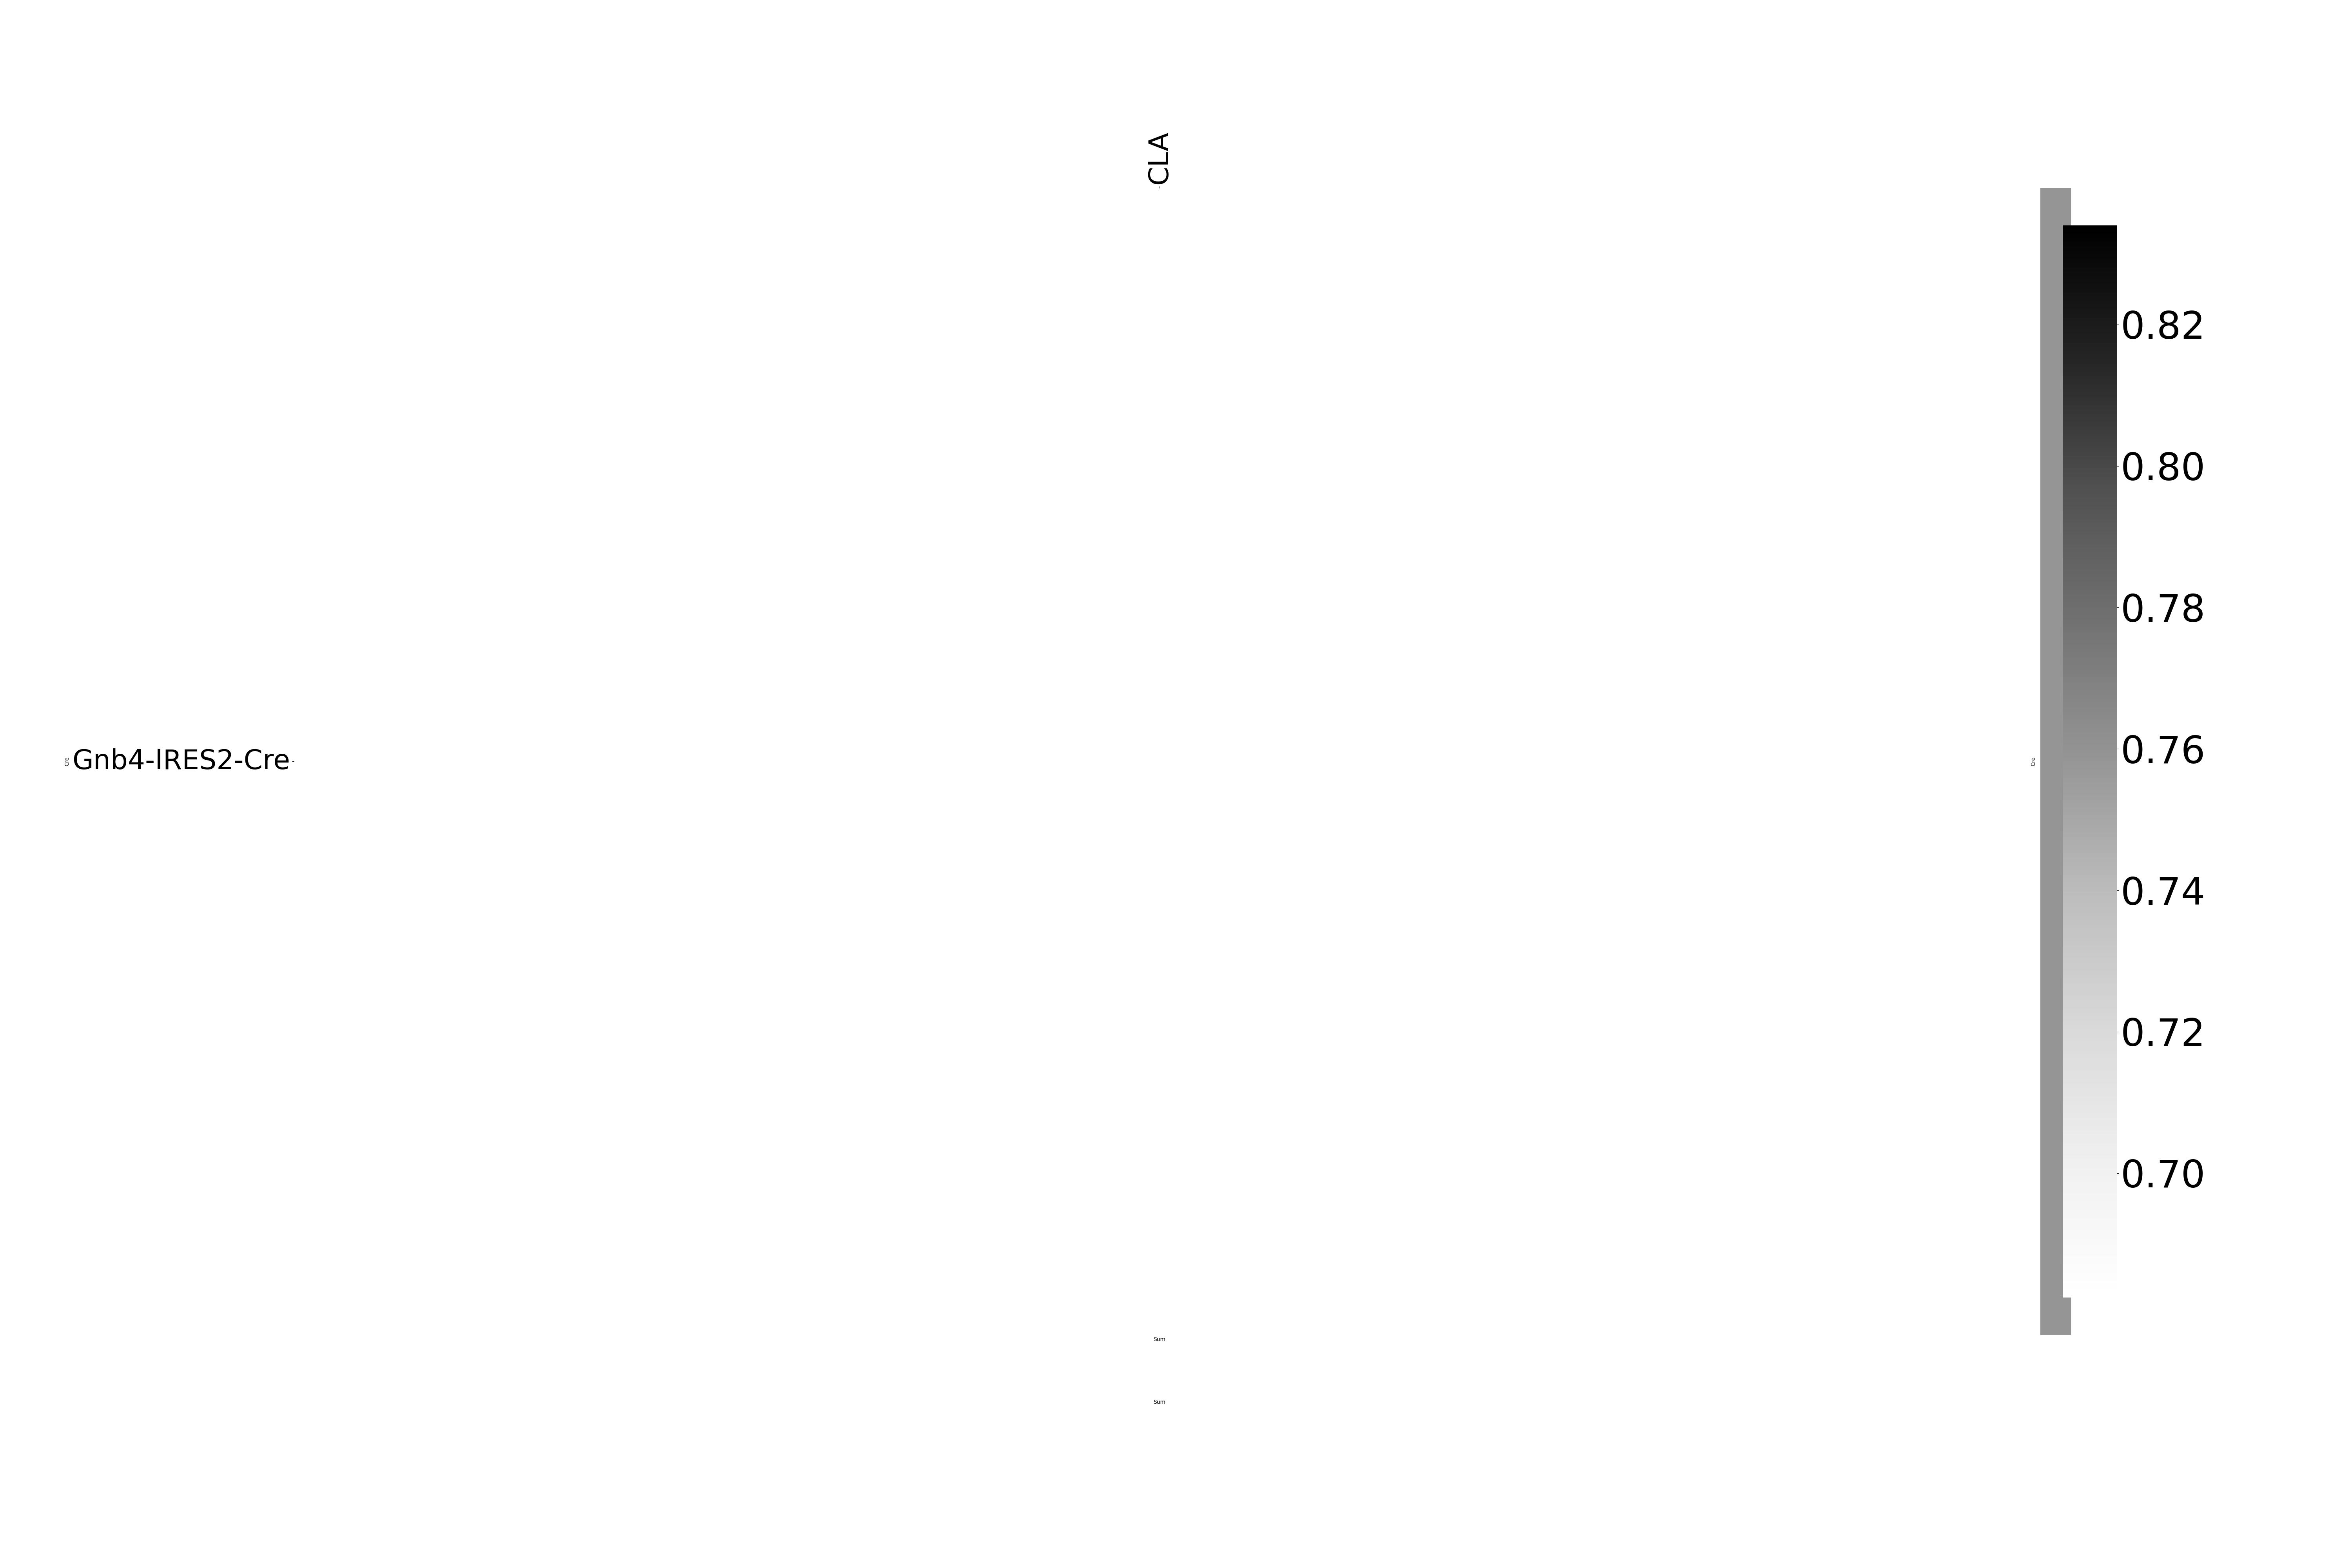
\includegraphics[width = 7in]{figs/lossdetails_703.png} 
    \label{fig:distances}
    \caption{}
\end{figure}

\begin{figure}[H]
    \centering
    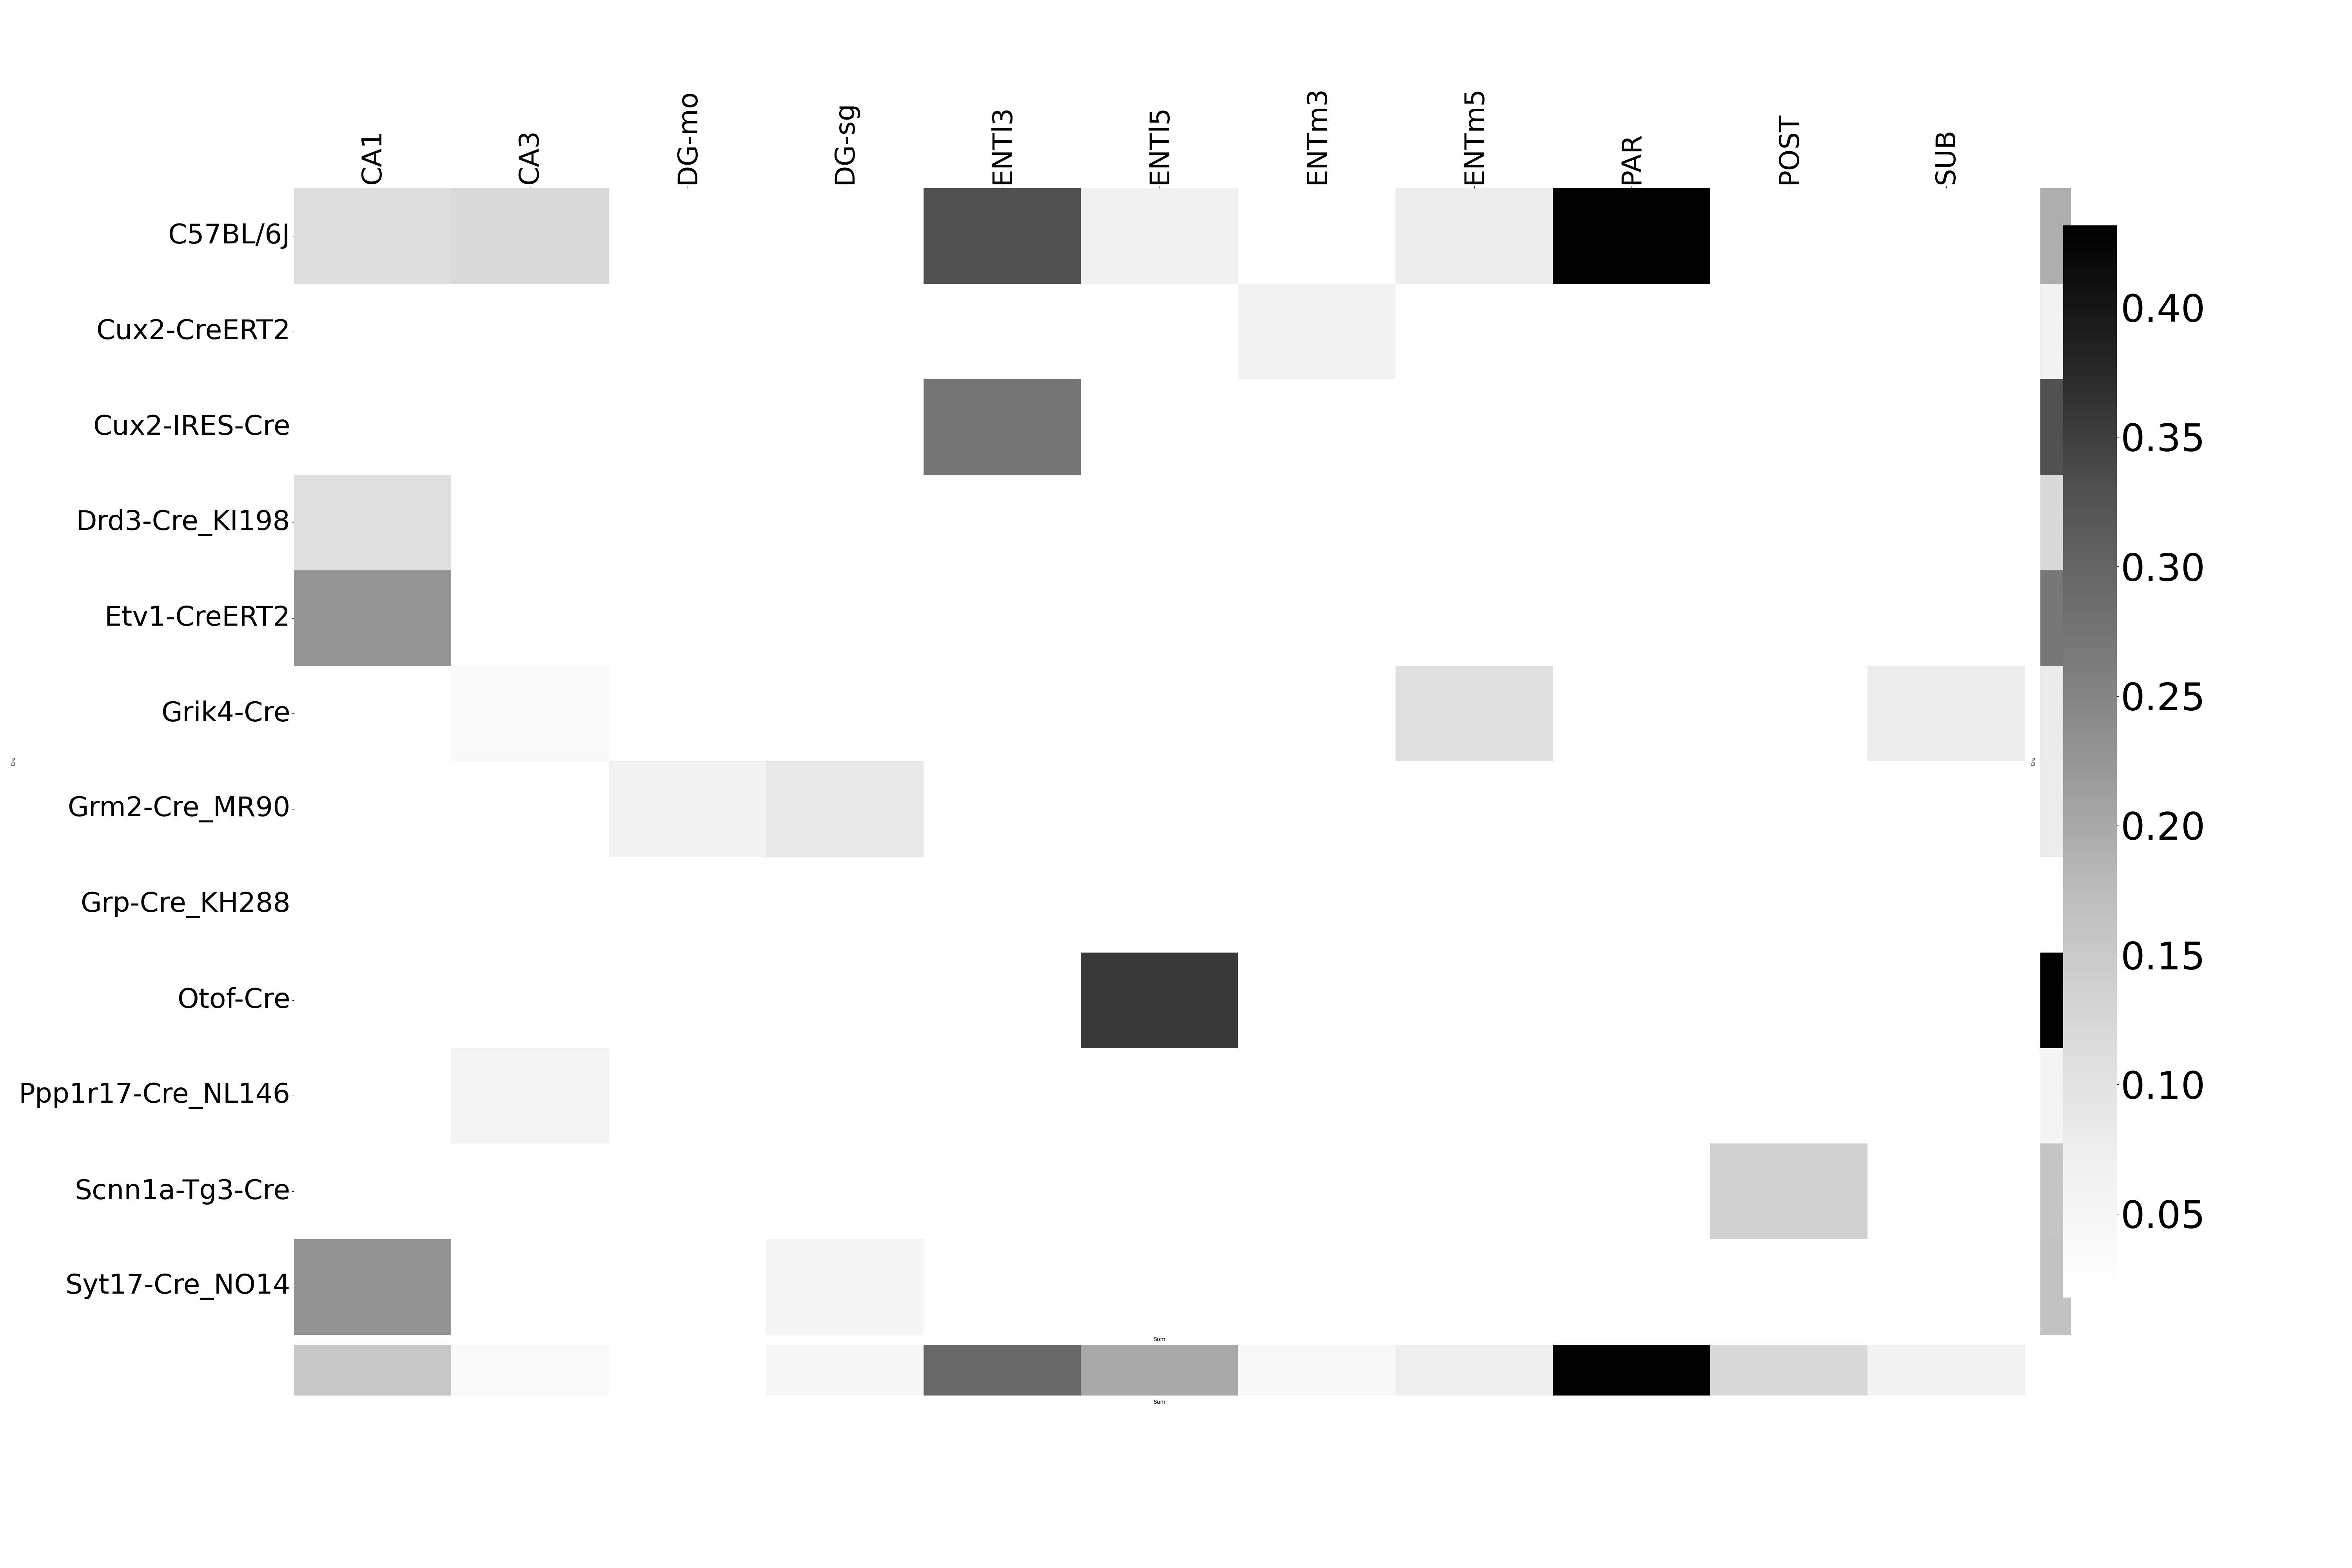
\includegraphics[width = 7in]{figs/lossdetails_1089.png} 
    \label{fig:distances}
    \caption{}
\end{figure}

\begin{figure}[H]
    \centering
    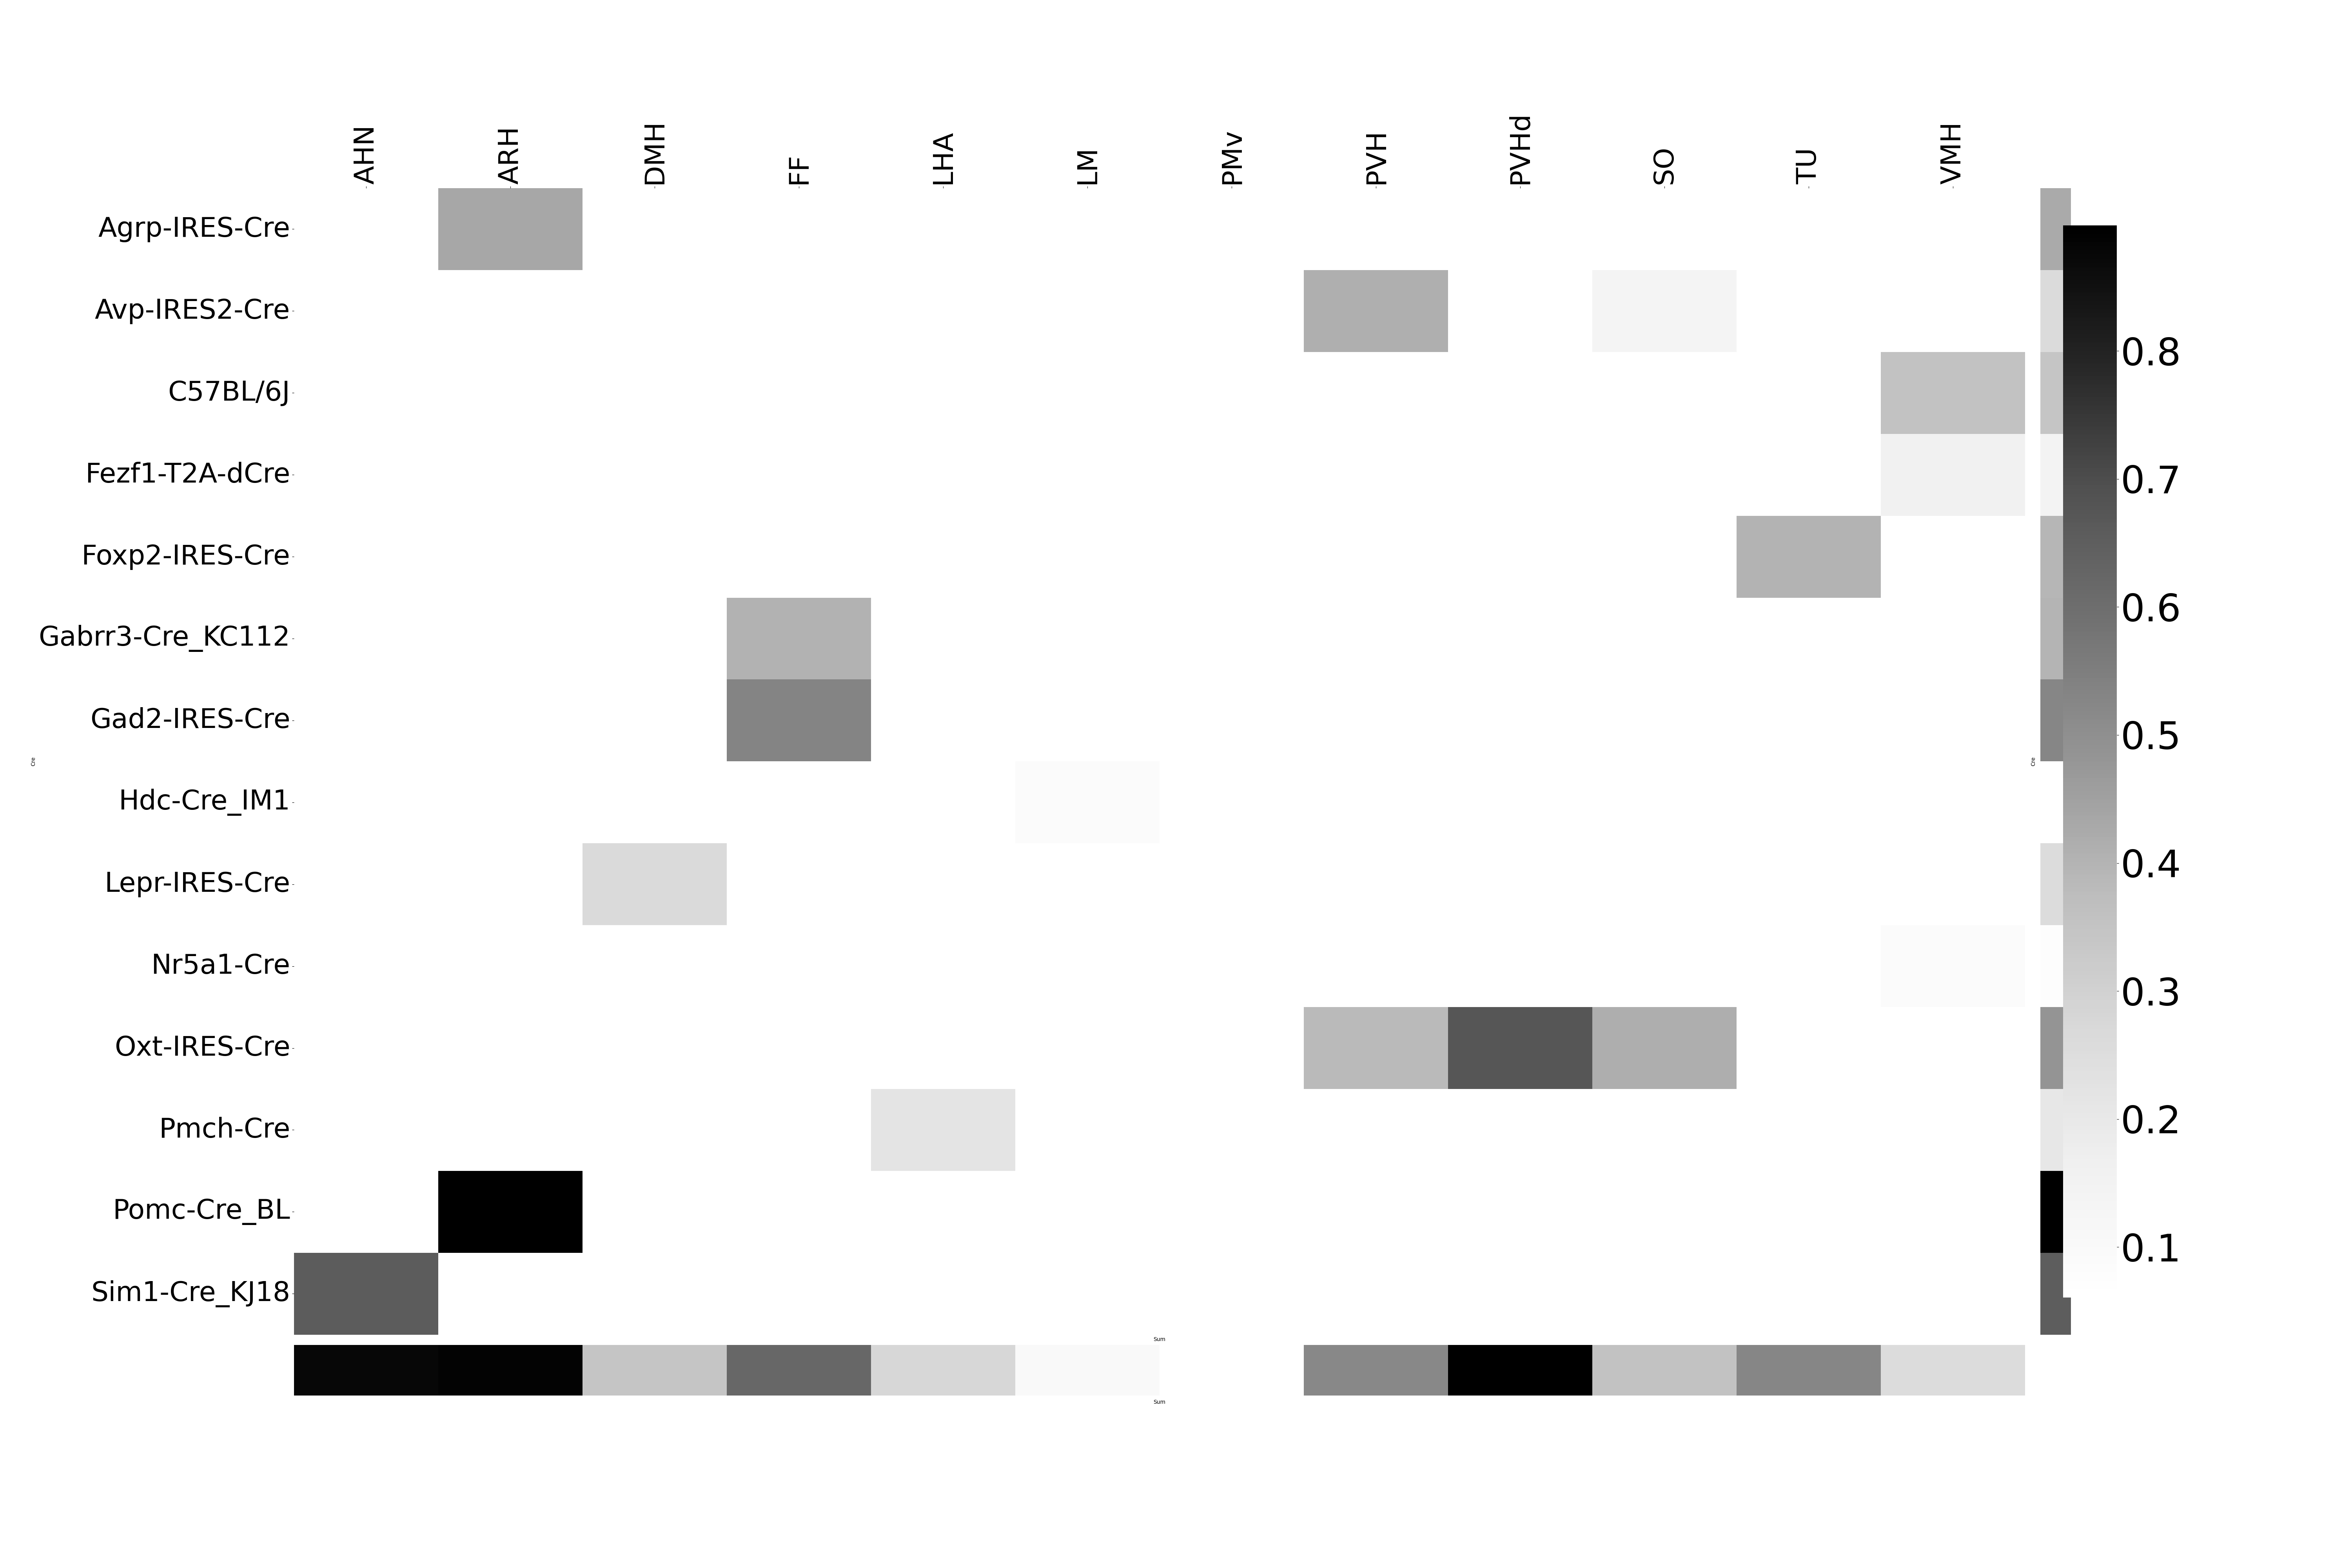
\includegraphics[width = 7in]{figs/lossdetails_1097.png} 
    \label{fig:distances}
    \caption{}
\end{figure}

\begin{figure}[H]
    \centering
    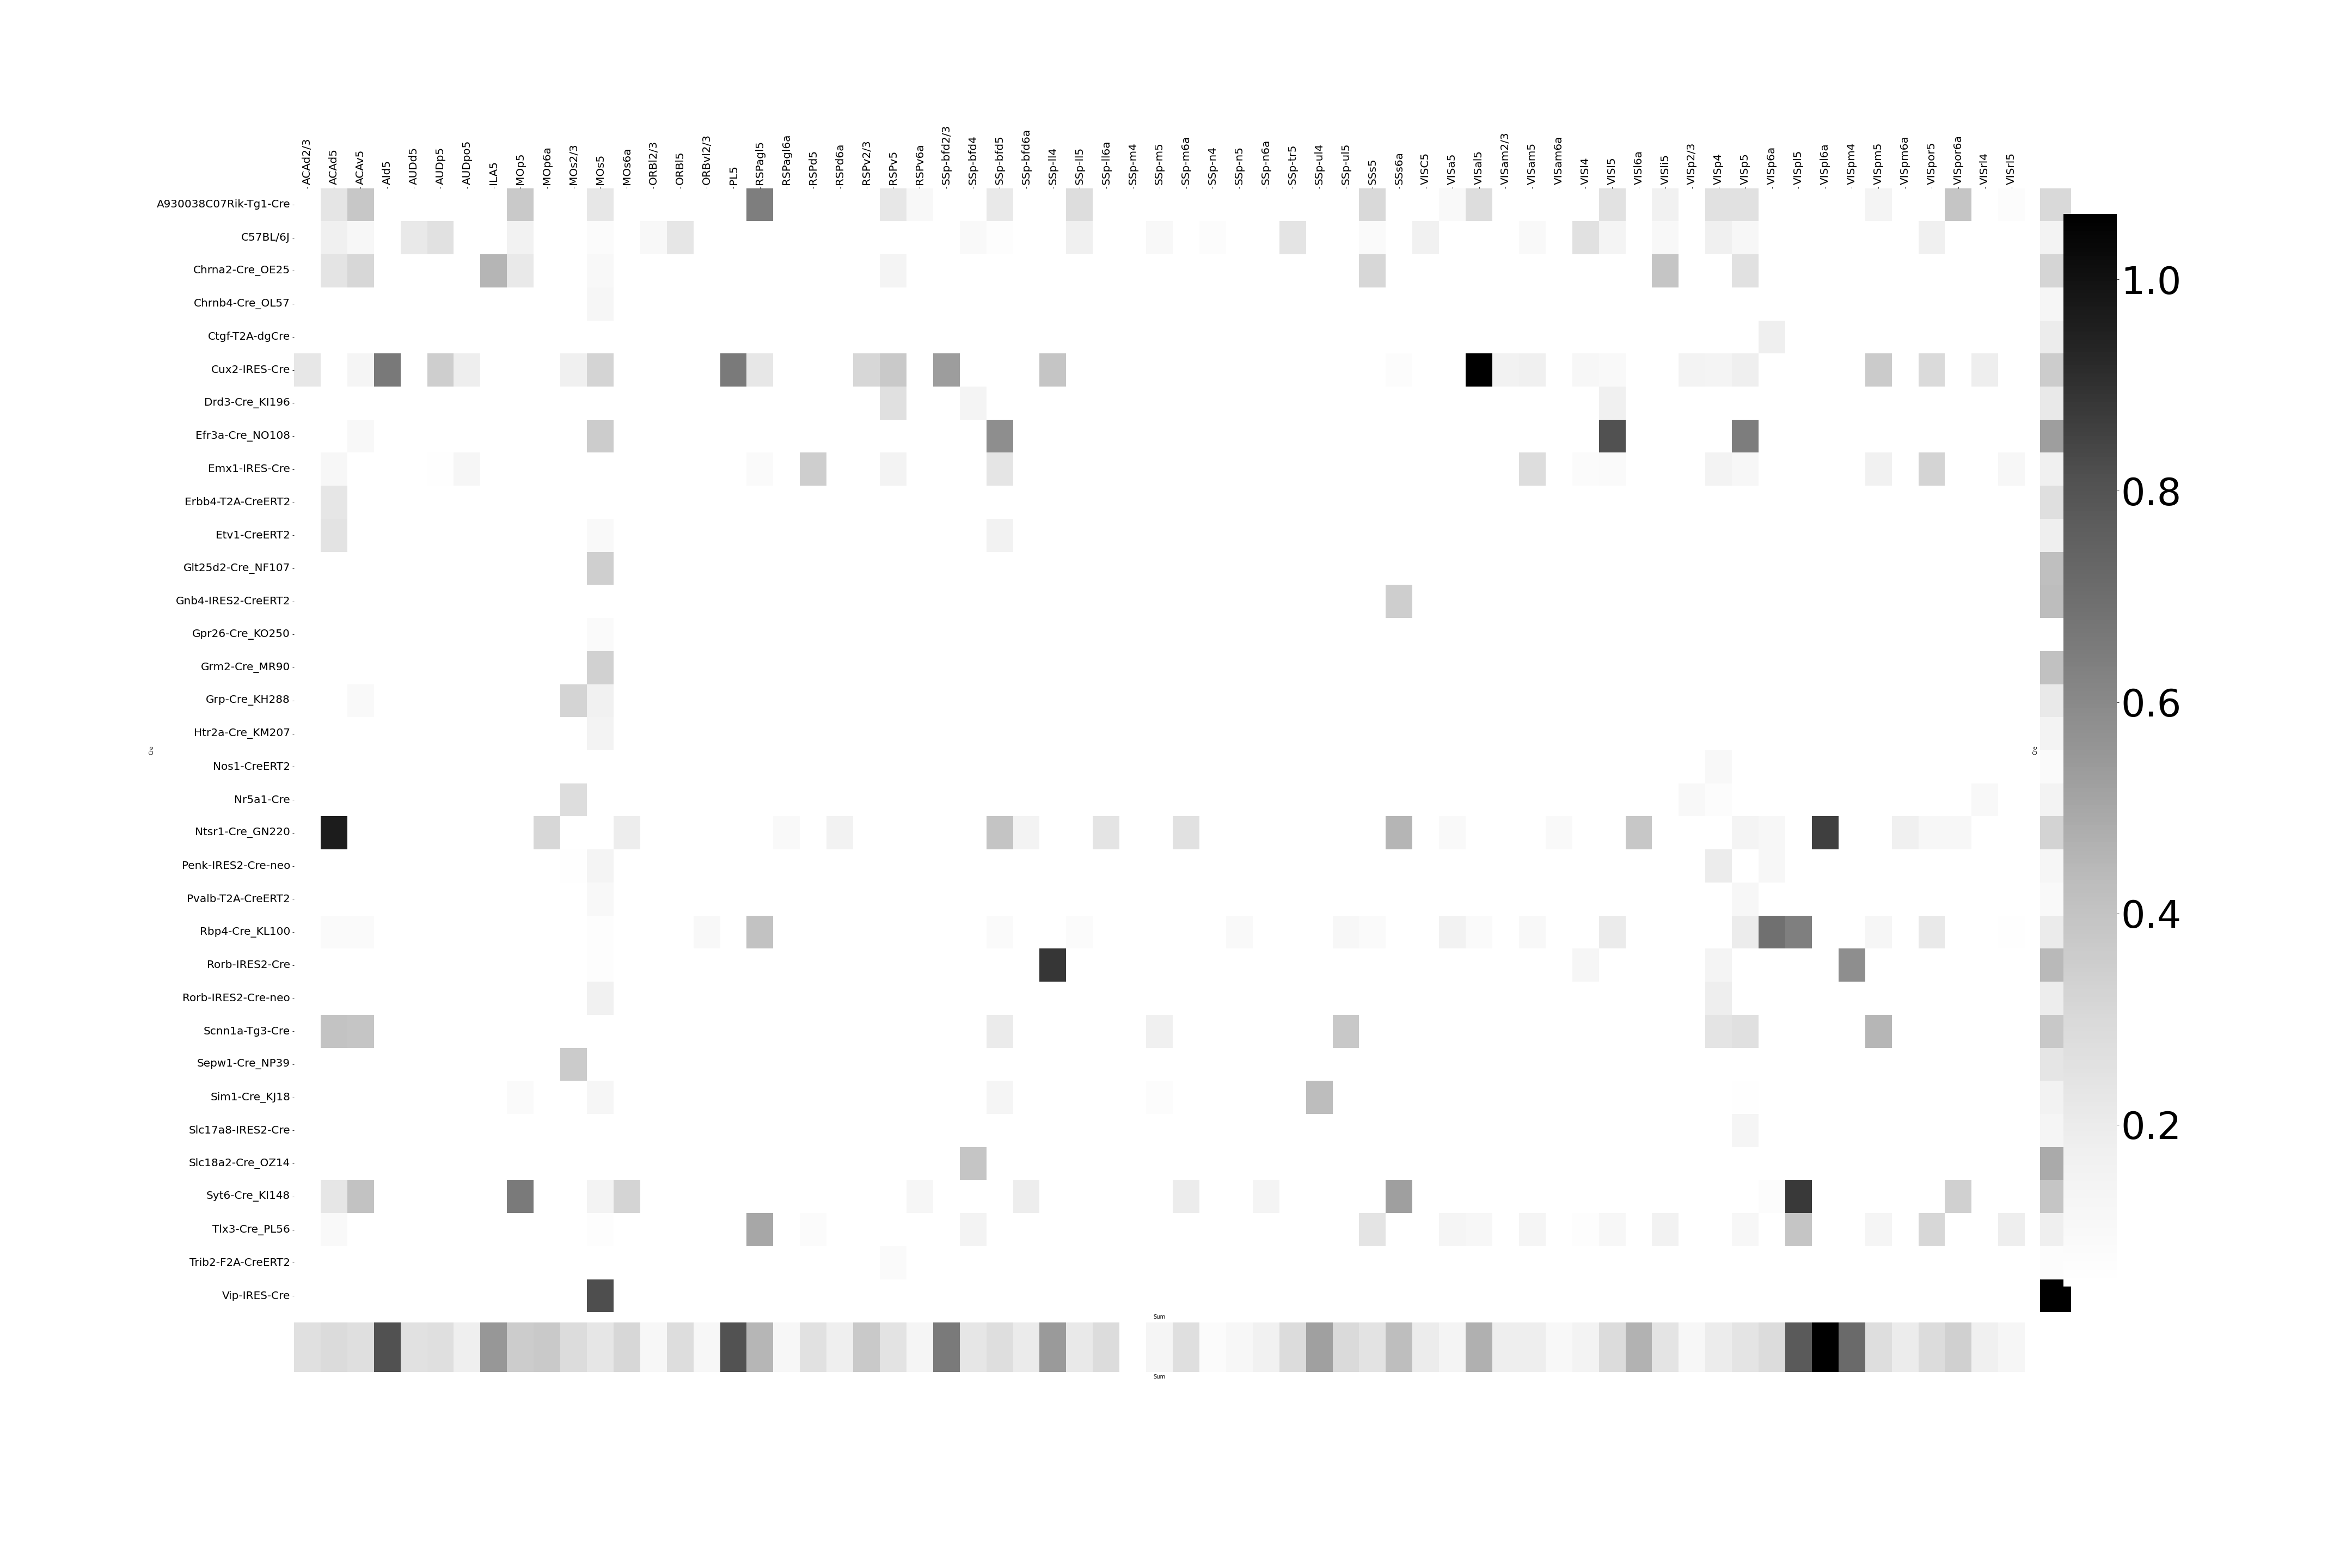
\includegraphics[width = 7in]{figs/lossdetails_315.png} 
    \label{fig:distances}
    \caption{}
\end{figure}

\begin{figure}[H]
    \centering
    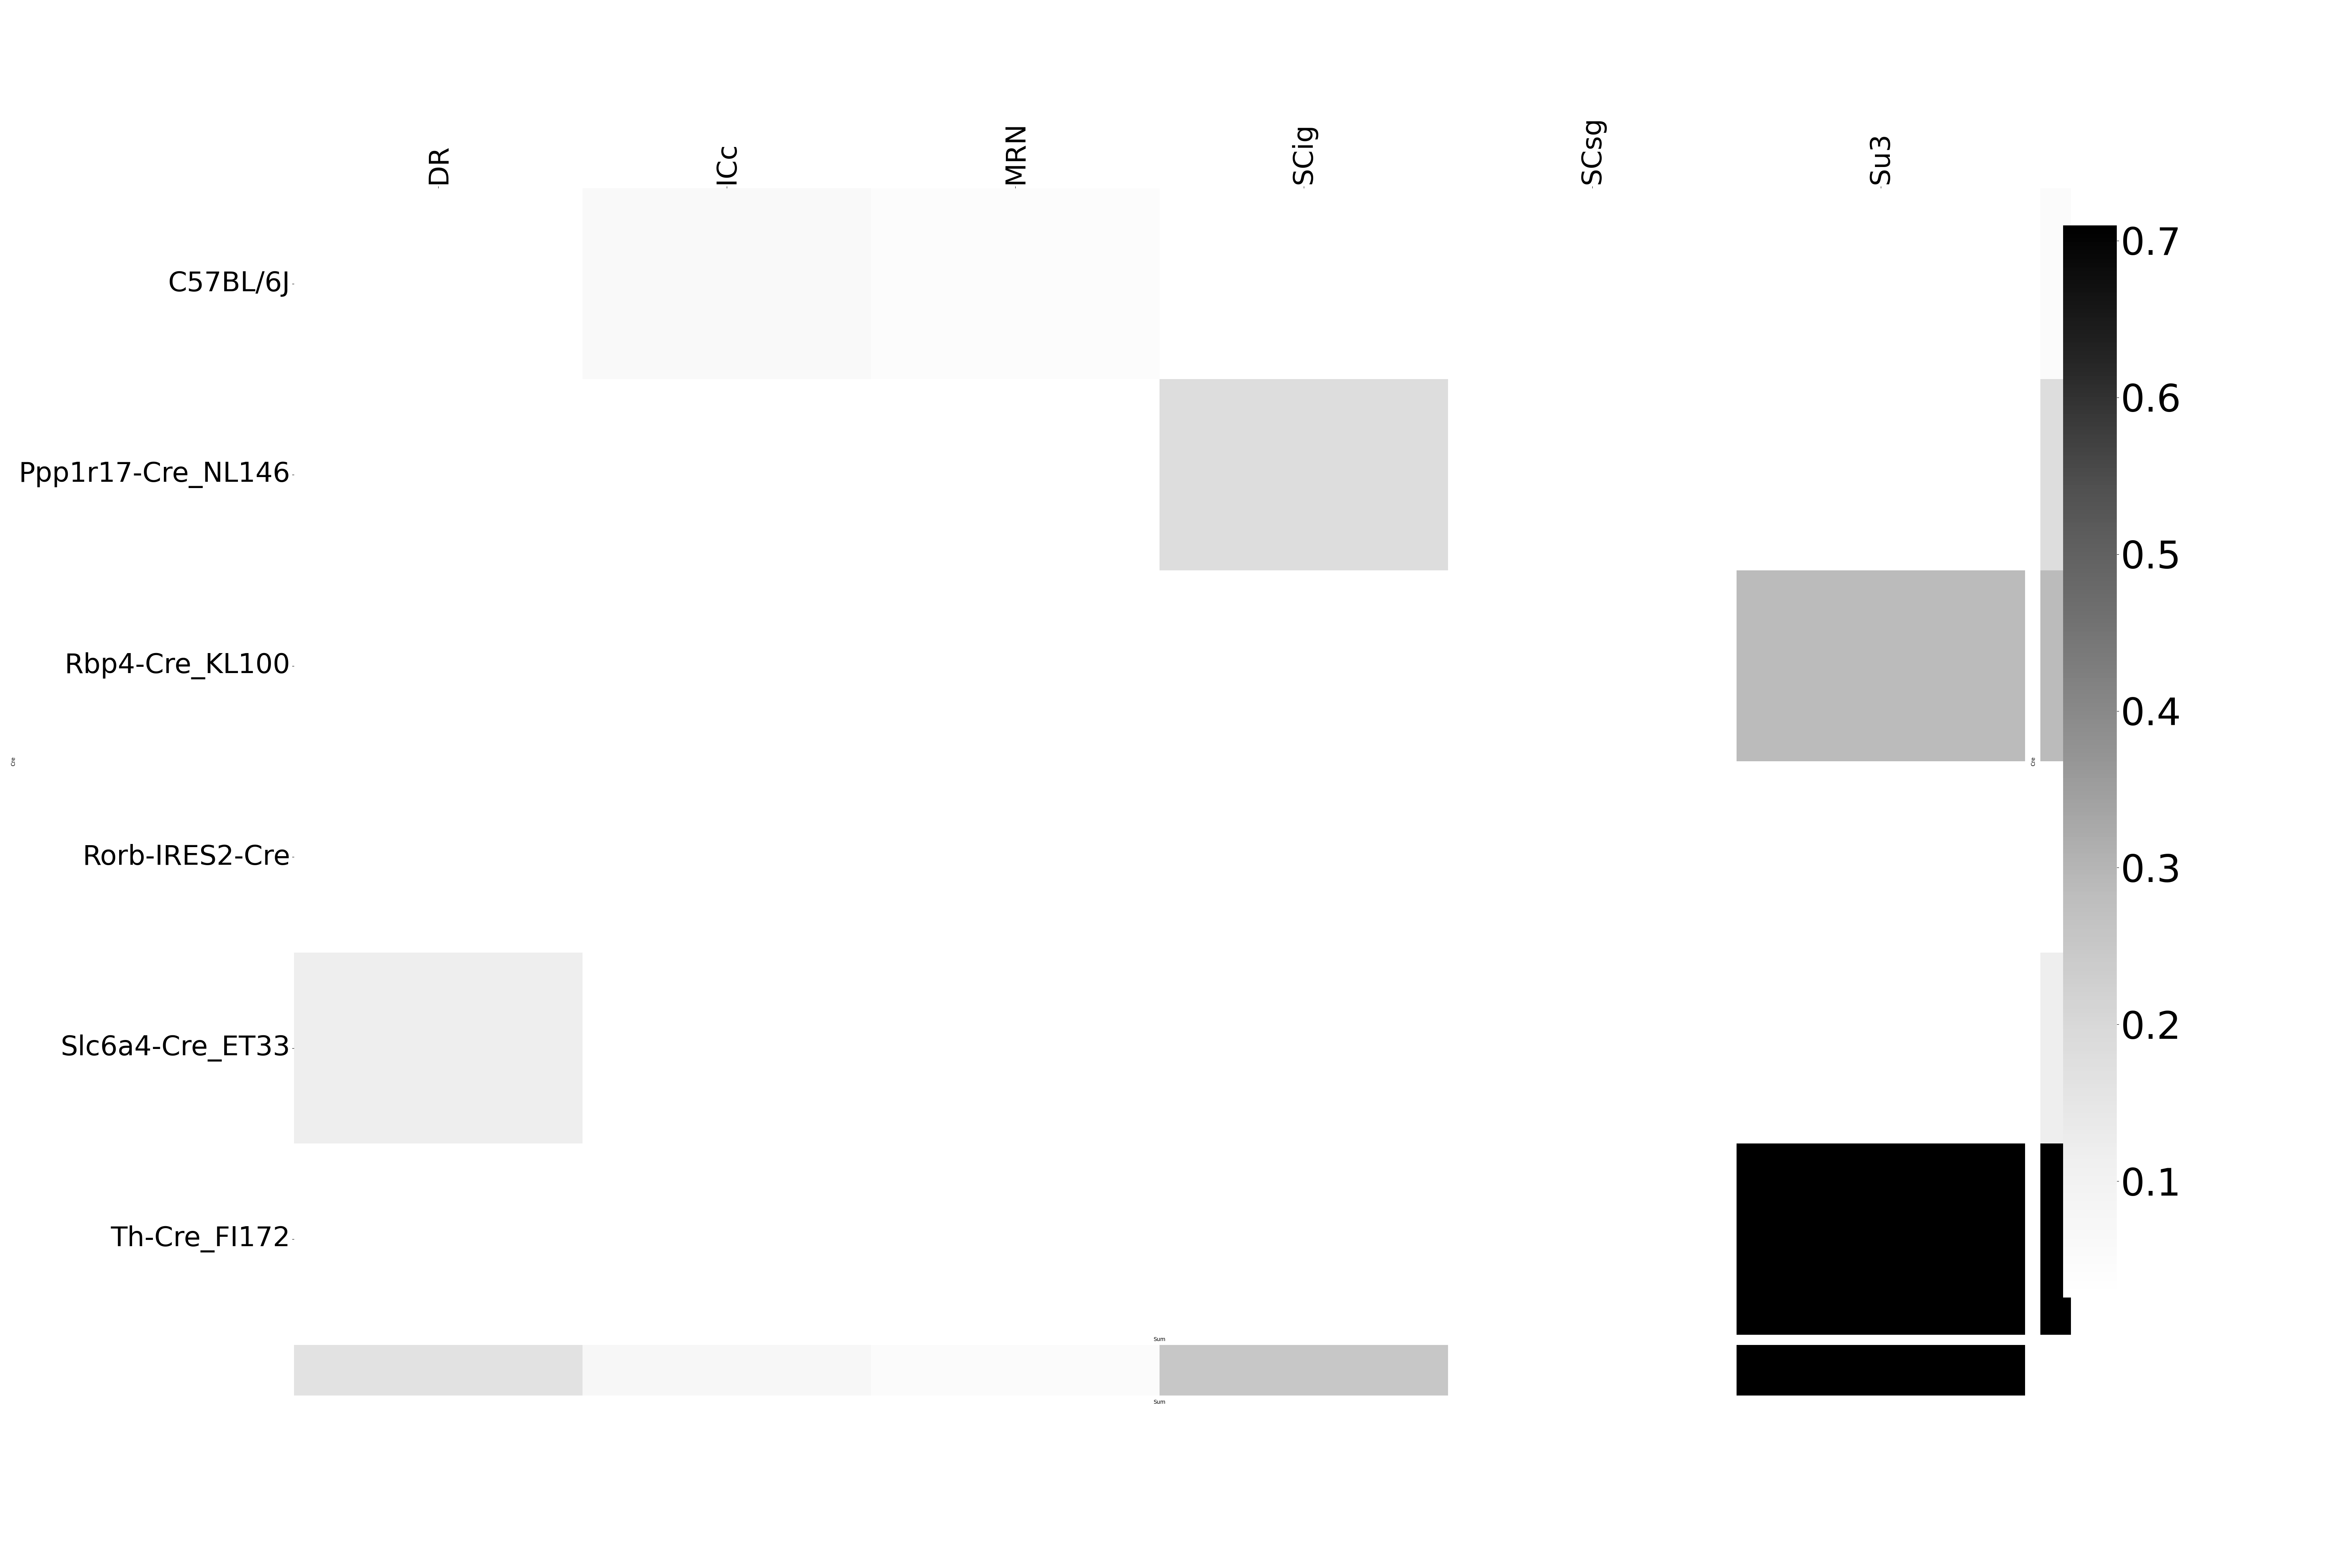
\includegraphics[width = 7in]{figs/lossdetails_313.png} 
    \label{fig:distances}
    \caption{}
\end{figure}

\begin{figure}[H]
    \centering
    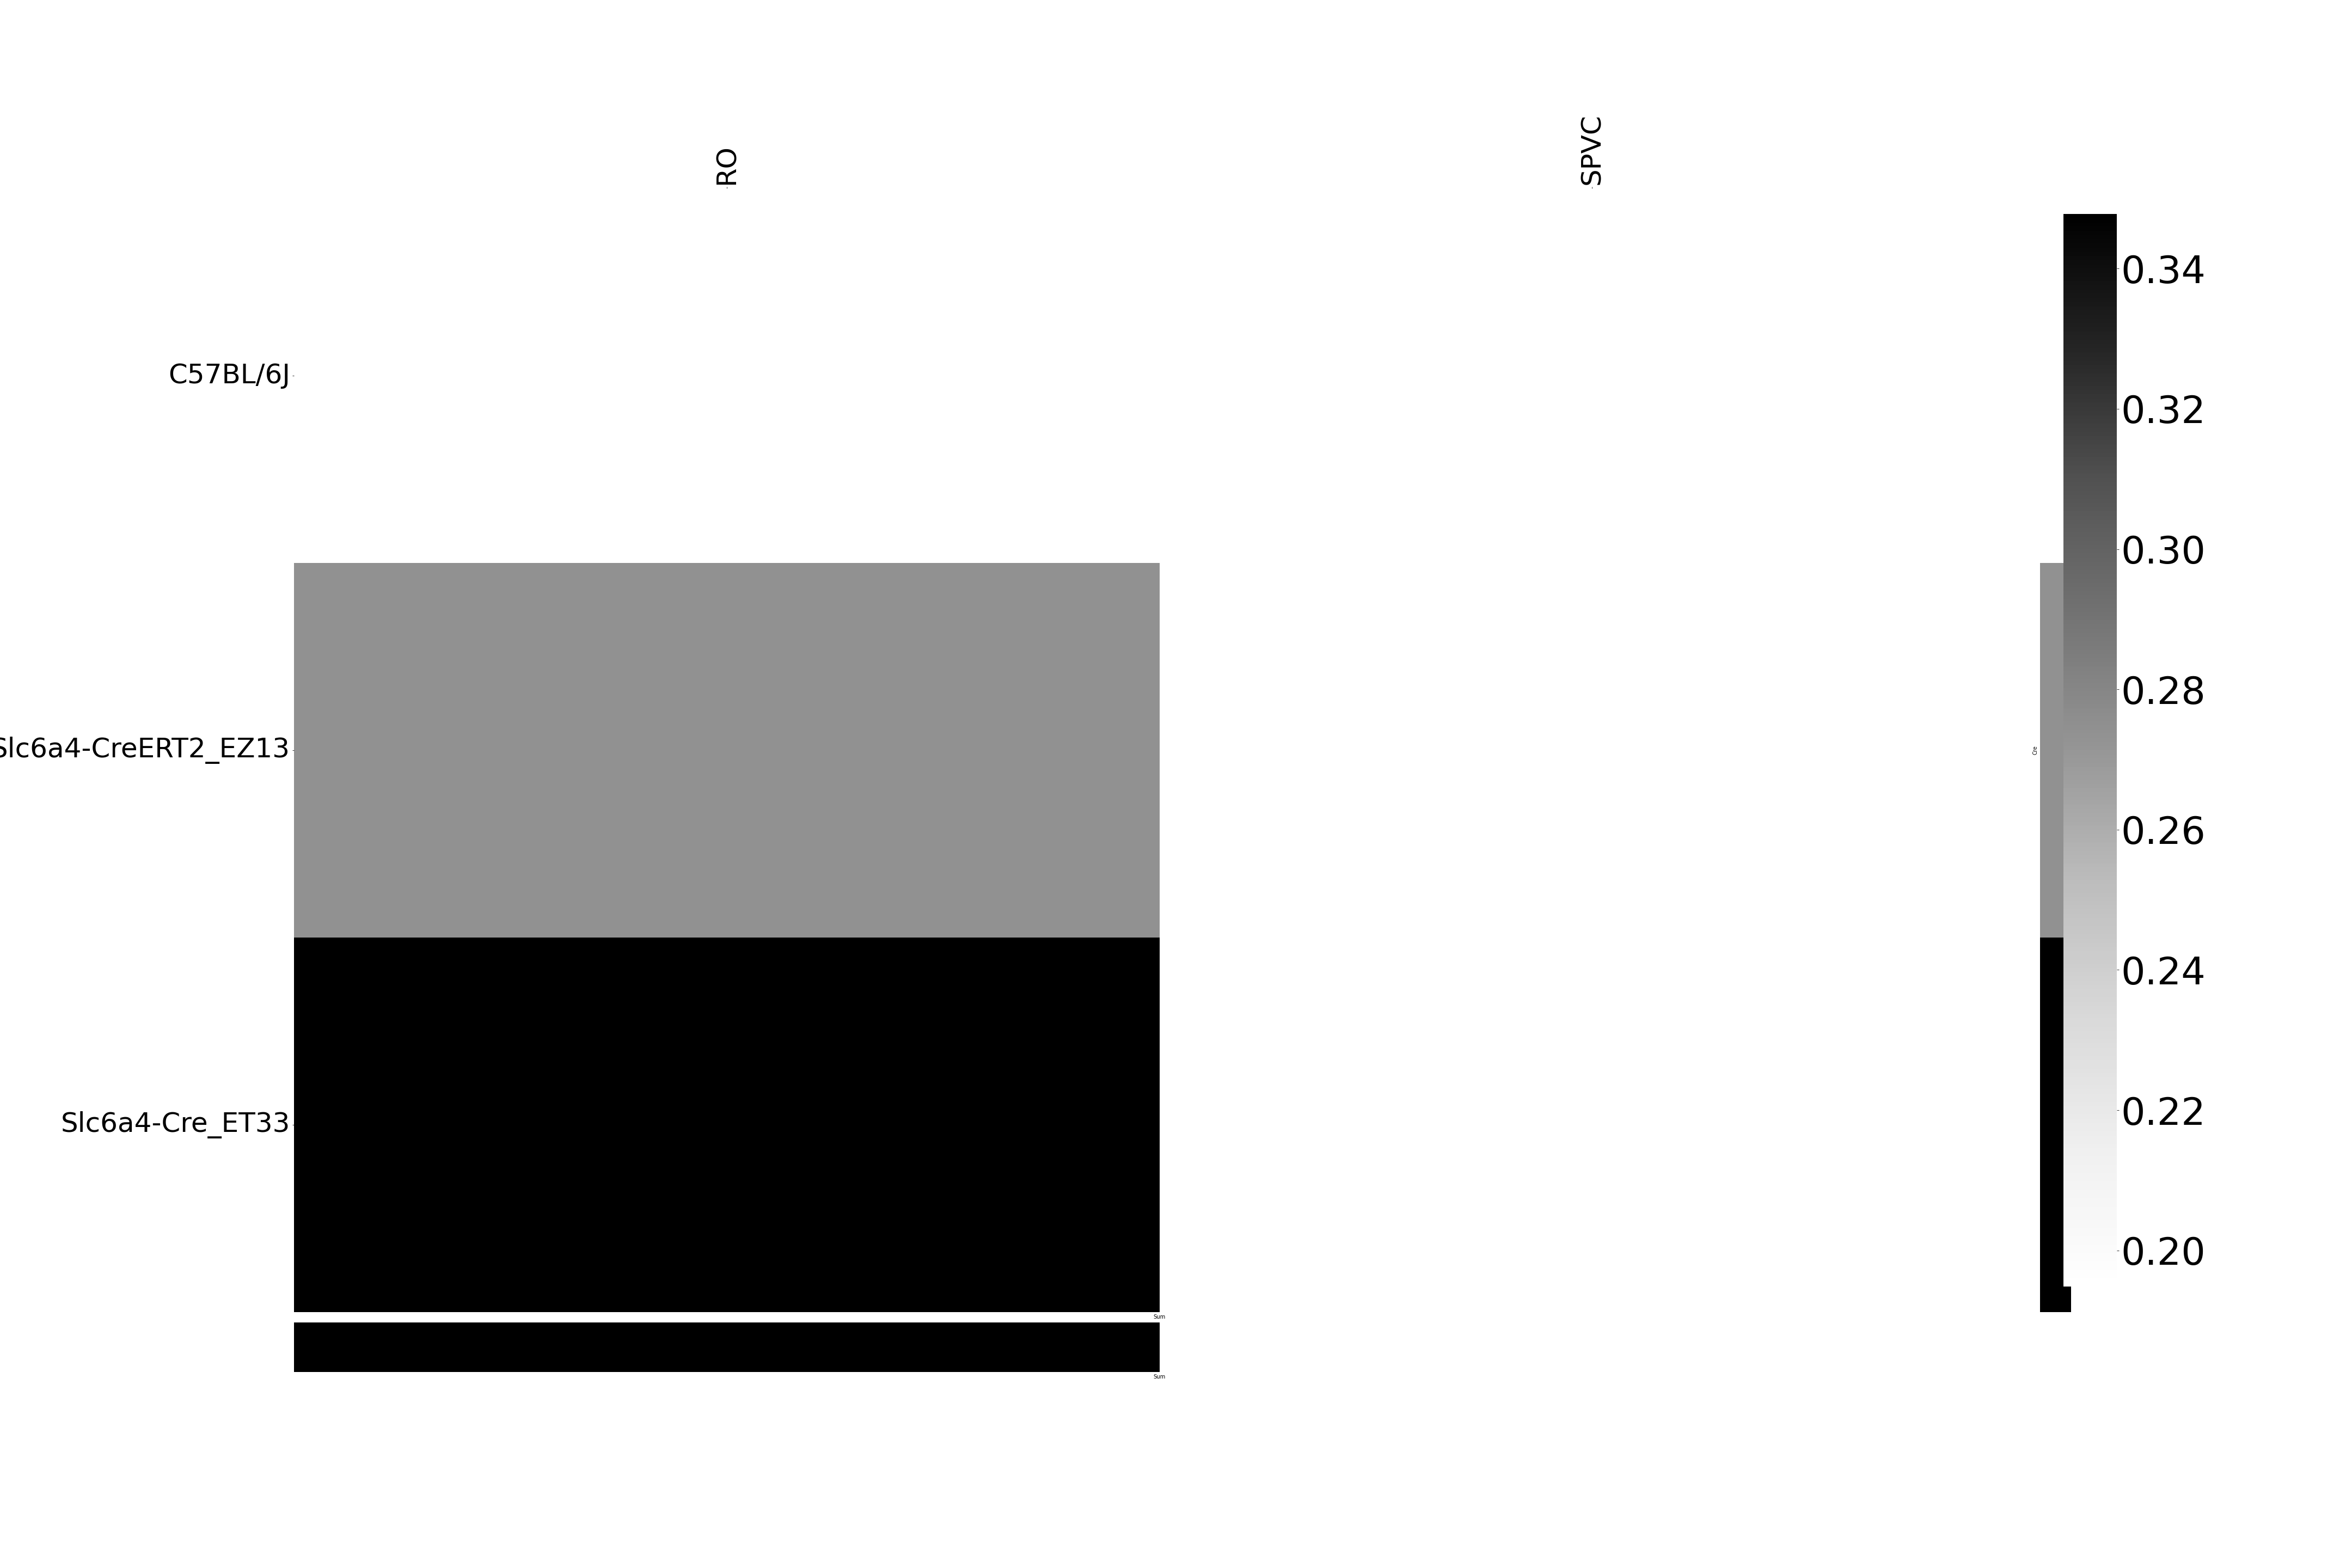
\includegraphics[width = 7in]{figs/lossdetails_354.png} 
    \label{fig:distances}
    \caption{}
\end{figure}

\begin{figure}[H]
    \centering
    \includegraphics[width = 7in]{paper/figures/lossdetails_0618_698.png} 
    \label{fig:distances}
    \caption{}
\end{figure}

\begin{figure}[H]
    \centering
    \includegraphics[width = 7in]{paper/figures/lossdetails_0618_771.png} 
    \label{fig:distances}
    \caption{}
\end{figure}

\begin{figure}[H]
    \centering
    \includegraphics[width = 7in]{paper/figures/lossdetails_0618_477.png} 
    \label{fig:distances}
    \caption{}
\end{figure}

\begin{figure}[H]
    \centering
    \includegraphics[width = 7in]{paper/figures/lossdetails_0618_549.png} 
    \label{fig:distances}
    \caption{}
\end{figure}

\newpage

\subsection{Matrix Factorization}
\label{supp_sec:matrix_factor_results}

We give additional results on the generation of the archetypal connectome patterns.
These consist of cross-validation selection of $q$, the number of latent components, stability analysis, and visualization of the reconstructed wild-type connectivity.

\subsubsection{Cross-validation}

We set $\alpha = 0.002$ and run Program \ref{eq:nmf} on $\mathcal C_{wt}$.
We use a random mask with $p = .3$ to evaluate prediction accuracy of models trained on the unmasked data on the masked data.
To account for stochasticity in the NMF algorithm, we run $R = 8$ replicates at each potential dimension $q$.
This selects $\hat q = 60$.

\begin{figure}[H]
    \centering
    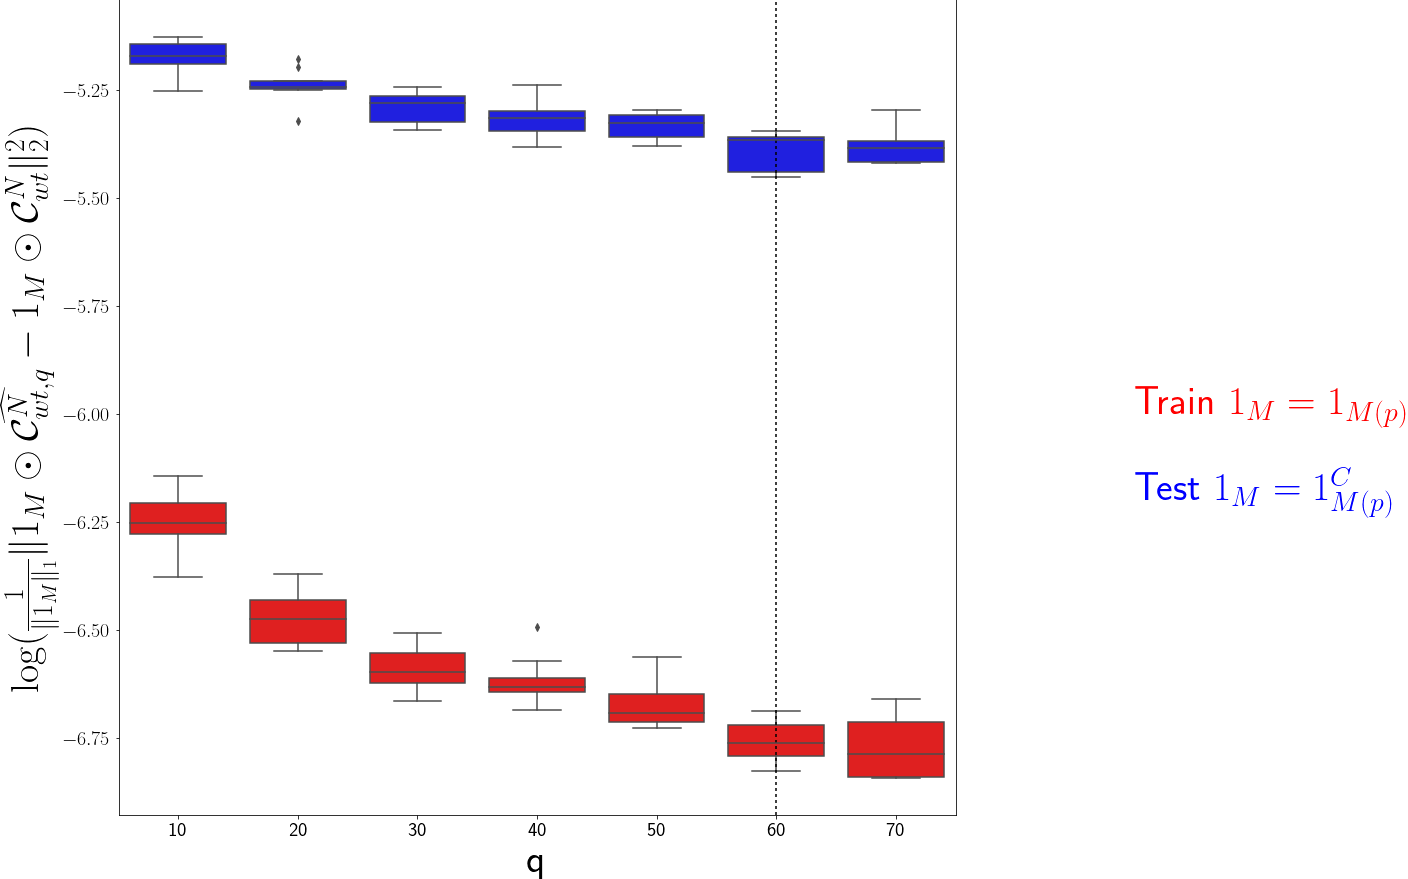
\includegraphics[width = 5in]{figs/nmf_test_train.png} 
    \label{fig:train_test}
    \caption{Train and test error using NMF decomposition.}
\end{figure}

\newpage

\subsubsection{Stability}

For the purposes of visualization and interpretability, we restrict to a $q = 15$ component model.
To address the instability of the NMF algorithm in identifying components, we $k-means$ cluster components over $R = 10$ replicates with $k \in \{10,15,20, 25, 30\}$.
Since the clustering is itself unstable, we repeat the clustering $25$ times and select the $k$ with the largest Rand index.

\begin{table}[H]
\begin{tabular}{lrrrrr}
\toprule
{} &          0 &          1 &          2 &         3 &          4 \\
\midrule
q          &  10 &  15 &  20 &  25 &  30 \\
Rand index &   0.685081 &   0.789262 &   0.921578 &   \textbf{0.94548} &   0.914799 \\
\bottomrule
\end{tabular}
\end{table}

Since $k$-means is most stable at $k=25$, we cluster the $qR = 150$ components into $25$ clusters and select the $15$ clusters appearing in the most replicates.
\begin{figure}[H]
    \centering
    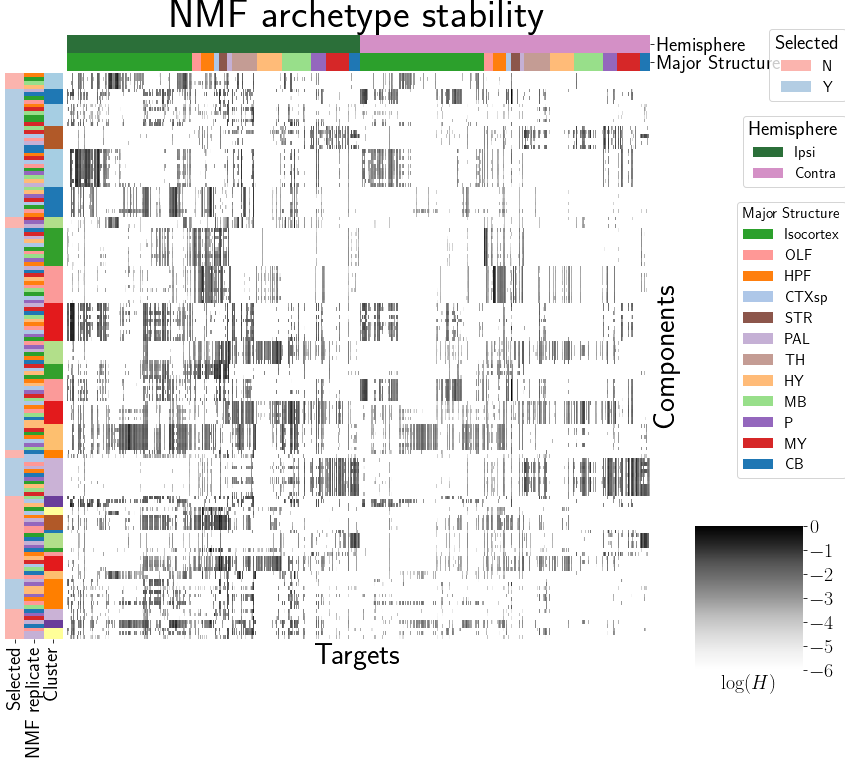
\includegraphics[width = 5in]{figs/nmfcluster.png} 
    \label{fig:distances}
    \caption{Stability of NMF results across replicates. 
    Replicate and NMF component are shown on rows.
    Components that are in the top $15$ are also indicated.}
\end{figure}
These are the components whose medians are plotted in Figure \ref{fig:H}.

\newpage

%A good $f$ will have low error on the training data, and also low error on the test data, indicating that it has not overfit.
%Although there is no assumed dichotomy between $X$ and $Y$ in unsupervised learning, for techniques like autoencoders, the above paradigm still applies, i.e., one can still hold out values of $X$.

%http://alexhwilliams.info/itsneuronalblog/2018/02/26/crossval/




\newpage
\section{Competing Interests}
\label{sec:comp}
This is an optional section. If you declared a conflict of interest when you submitted your manuscript, please  use this space to provide details about this conflict.

\newpage
\bibliography{connectivity}

\newpage
\section{Technical Terms}

\textbf{Technical Term} a key term that is mentioned in an NETN article and whose usage and definition may not be familiar across the broad readership of the journal. 

\textbf{Cre-line}  Refers to the combination of cre-recombinase expression in transgenic mouse and cre-induced promotion in the vector that induces labelling of cell-class specific projection. 

\textbf{Cell class} The projecting neurons targeted by a particular cre-line 

\textbf{Structural connectivities}  connectivity between structures 

\textbf{Voxel} A $100 \mu m$ cube of brain. 

\textbf{Structural connection tensor}  Connectivities between structures given a neuron class

\textbf{dictionary-learning} A family of algorithms for finding low-dimensional data representations.

\textbf{Shape constrained estimator} A statistical estimator that fits a function of a particular shape (e.g. monotonic increasing, convex).

\textbf{Nadaraya-Watson} A simple smoothing estimator.

\textbf{Connectivity archetypes} Typical connectivity patterns

 \textbf{Expected loss} Our new estimator that weights different features by their estimated predictive power.
 
%All NETN article types require Technical Terms.

%Identify approximately 10 key terms that are mentioned in your article and whose usage and definition may not be familiar across the broad readership of the journal. 
%Provide brief (20-word or less) definitions for each term, avoiding in these definitions the use of jargon, or highly technical or specialized language. 
%When the article is typeset, the Technical Terms will appear in the margins at or near their first mention in the text.

%In your manuscript, bold the first occurrence of each \textbf{Technical Term} and then provide a list of the terms and their definitions at the end of the manuscript after the references. 


\end{document}


%\newpage
